\documentclass[twoside]{book}

% Packages required by doxygen
\usepackage{fixltx2e}
\usepackage{calc}
\usepackage{doxygen}
\usepackage[export]{adjustbox} % also loads graphicx
\usepackage{graphicx}
\usepackage[utf8]{inputenc}
\usepackage{makeidx}
\usepackage{multicol}
\usepackage{multirow}
\PassOptionsToPackage{warn}{textcomp}
\usepackage{textcomp}
\usepackage[nointegrals]{wasysym}
\usepackage[table]{xcolor}

% Font selection
\usepackage[T1]{fontenc}
\usepackage[scaled=.90]{helvet}
\usepackage{courier}
\usepackage{amssymb}
\usepackage{sectsty}
\renewcommand{\familydefault}{\sfdefault}
\allsectionsfont{%
  \fontseries{bc}\selectfont%
  \color{darkgray}%
}
\renewcommand{\DoxyLabelFont}{%
  \fontseries{bc}\selectfont%
  \color{darkgray}%
}
\newcommand{\+}{\discretionary{\mbox{\scriptsize$\hookleftarrow$}}{}{}}

% Page & text layout
\usepackage{geometry}
\geometry{%
  a4paper,%
  top=2.5cm,%
  bottom=2.5cm,%
  left=2.5cm,%
  right=2.5cm%
}
\tolerance=750
\hfuzz=15pt
\hbadness=750
\setlength{\emergencystretch}{15pt}
\setlength{\parindent}{0cm}
\setlength{\parskip}{3ex plus 2ex minus 2ex}
\makeatletter
\renewcommand{\paragraph}{%
  \@startsection{paragraph}{4}{0ex}{-1.0ex}{1.0ex}{%
    \normalfont\normalsize\bfseries\SS@parafont%
  }%
}
\renewcommand{\subparagraph}{%
  \@startsection{subparagraph}{5}{0ex}{-1.0ex}{1.0ex}{%
    \normalfont\normalsize\bfseries\SS@subparafont%
  }%
}
\makeatother

% Headers & footers
\usepackage{fancyhdr}
\pagestyle{fancyplain}
\fancyhead[LE]{\fancyplain{}{\bfseries\thepage}}
\fancyhead[CE]{\fancyplain{}{}}
\fancyhead[RE]{\fancyplain{}{\bfseries\leftmark}}
\fancyhead[LO]{\fancyplain{}{\bfseries\rightmark}}
\fancyhead[CO]{\fancyplain{}{}}
\fancyhead[RO]{\fancyplain{}{\bfseries\thepage}}
\fancyfoot[LE]{\fancyplain{}{}}
\fancyfoot[CE]{\fancyplain{}{}}
\fancyfoot[RE]{\fancyplain{}{\bfseries\scriptsize Generated by Doxygen }}
\fancyfoot[LO]{\fancyplain{}{\bfseries\scriptsize Generated by Doxygen }}
\fancyfoot[CO]{\fancyplain{}{}}
\fancyfoot[RO]{\fancyplain{}{}}
\renewcommand{\footrulewidth}{0.4pt}
\renewcommand{\chaptermark}[1]{%
  \markboth{#1}{}%
}
\renewcommand{\sectionmark}[1]{%
  \markright{\thesection\ #1}%
}

% Indices & bibliography
\usepackage{natbib}
\usepackage[titles]{tocloft}
\setcounter{tocdepth}{3}
\setcounter{secnumdepth}{5}
\makeindex

% Hyperlinks (required, but should be loaded last)
\usepackage{ifpdf}
\ifpdf
  \usepackage[pdftex,pagebackref=true]{hyperref}
\else
  \usepackage[ps2pdf,pagebackref=true]{hyperref}
\fi
\hypersetup{%
  colorlinks=true,%
  linkcolor=blue,%
  citecolor=blue,%
  unicode%
}

% Custom commands
\newcommand{\clearemptydoublepage}{%
  \newpage{\pagestyle{empty}\cleardoublepage}%
}

\usepackage{caption}
\captionsetup{labelsep=space,justification=centering,font={bf},singlelinecheck=off,skip=4pt,position=top}

%===== C O N T E N T S =====

\begin{document}

% Titlepage & ToC
\hypersetup{pageanchor=false,
             bookmarksnumbered=true,
             pdfencoding=unicode
            }
\pagenumbering{alph}
\begin{titlepage}
\vspace*{7cm}
\begin{center}%
{\Large M\+\_\+time }\\
\vspace*{1cm}
{\large Generated by Doxygen 1.8.14}\\
\end{center}
\end{titlepage}
\clearemptydoublepage
\pagenumbering{roman}
\tableofcontents
\clearemptydoublepage
\pagenumbering{arabic}
\hypersetup{pageanchor=true}

%--- Begin generated contents ---
\chapter{M\+\_\+time Fortran Library}
\label{index}\hypertarget{index}{}~~~~

~~~~\hypertarget{index_Introduction}{}\doxysection{Introduction}\label{index_Introduction}
Date and time procedures that expand upon the Fortran D\+A\+T\+E\+\_\+\+A\+N\+D\+\_\+\+T\+I\+M\+E(3f) intrinsic.

~~~~  
\chapter{Modules Index}
\doxysection{Modules List}
Here is a list of all modules with brief descriptions\+:\begin{DoxyCompactList}
\item\contentsline{section}{\mbox{\hyperlink{namespacem__time}{m\+\_\+time}} }{\pageref{namespacem__time}}{}
\item\contentsline{section}{\mbox{\hyperlink{namespacem__time__duplicate}{m\+\_\+time\+\_\+duplicate}} }{\pageref{namespacem__time__duplicate}}{}
\item\contentsline{section}{\mbox{\hyperlink{namespacem__time__oop}{m\+\_\+time\+\_\+oop}} }{\pageref{namespacem__time__oop}}{}
\end{DoxyCompactList}

\chapter{Data Type Index}
\doxysection{Data Types List}
Here are the data types with brief descriptions\+:\begin{DoxyCompactList}
\item\contentsline{section}{\mbox{\hyperlink{structm__time__oop_1_1date__time}{m\+\_\+time\+\_\+oop\+::date\+\_\+time}} }{\pageref{structm__time__oop_1_1date__time}}{}
\item\contentsline{section}{\mbox{\hyperlink{interfacem__time__duplicate_1_1string__to__value}{m\+\_\+time\+\_\+duplicate\+::string\+\_\+to\+\_\+value}} }{\pageref{interfacem__time__duplicate_1_1string__to__value}}{}
\item\contentsline{section}{\mbox{\hyperlink{interfacem__time__duplicate_1_1v2s}{m\+\_\+time\+\_\+duplicate\+::v2s}} }{\pageref{interfacem__time__duplicate_1_1v2s}}{}
\end{DoxyCompactList}

\chapter{File Index}
\doxysection{File List}
Here is a list of all files with brief descriptions\+:\begin{DoxyCompactList}
\item\contentsline{section}{/home/urbanjs/venus/\+V600/github/\+M\+\_\+time/src/\mbox{\hyperlink{M__time_8f90}{M\+\_\+time.\+f90}} }{\pageref{M__time_8f90}}{}
\item\contentsline{section}{/home/urbanjs/venus/\+V600/github/\+M\+\_\+time/src/\mbox{\hyperlink{M__time__duplicate_8f90}{M\+\_\+time\+\_\+duplicate.\+f90}} }{\pageref{M__time__duplicate_8f90}}{}
\item\contentsline{section}{/home/urbanjs/venus/\+V600/github/\+M\+\_\+time/src/\mbox{\hyperlink{M__time__oop_8f90}{M\+\_\+time\+\_\+oop.\+f90}} }{\pageref{M__time__oop_8f90}}{}
\end{DoxyCompactList}

\chapter{Module Documentation}
\hypertarget{namespacem__time}{}\doxysection{m\+\_\+time Module Reference}
\label{namespacem__time}\index{m\_time@{m\_time}}
\doxysubsection*{Functions/\+Subroutines}
\begin{DoxyCompactItemize}
\item 
subroutine, public \mbox{\hyperlink{namespacem__time_acfdc970b4154b0c15bd33727636e3992}{date\+\_\+to\+\_\+julian}} (dat, julian, ierr)
\item 
subroutine, public \mbox{\hyperlink{namespacem__time_abb44cf18cd0a3e420c20469efb056203}{julian\+\_\+to\+\_\+date}} (julian, dat, ierr)
\item 
subroutine, public \mbox{\hyperlink{namespacem__time_aed245c691853279ebf0ce899dec9caa9}{date\+\_\+to\+\_\+unix}} (dat, unixtime, ierr)
\item 
subroutine, public \mbox{\hyperlink{namespacem__time_acc62ada23f8fa2fe67b428702fbcbf1c}{unix\+\_\+to\+\_\+date}} (unixtime, dat, ierr)
\item 
integer function, public \mbox{\hyperlink{namespacem__time_a727dd77bbd4a5d0e3947c5d303845947}{d2o}} (dat)
\item 
integer function, public \mbox{\hyperlink{namespacem__time_ab8960d2aa60e134bcf77247d8b257963}{ordinal\+\_\+seconds}} ()
\item 
subroutine, public \mbox{\hyperlink{namespacem__time_aa4dca4409bf20a011bb04988c1335d63}{ordinal\+\_\+to\+\_\+date}} (yyyy, ddd, dat)
\item 
integer function, dimension(8), public \mbox{\hyperlink{namespacem__time_a55e2cb9efc9d4d209ae2864f073d4f19}{o2d}} (ordinal, year)
\item 
character(len=\+:) function, allocatable, public \mbox{\hyperlink{namespacem__time_a6f28cf00e4998bb50bb503f5e4bd3f77}{v2mo}} (imonth)
\item 
integer function, dimension(8), public \mbox{\hyperlink{namespacem__time_a8188c7ed4e592c4f2388d28c75486726}{mo2d}} (month\+\_\+name, year)
\item 
integer function, public \mbox{\hyperlink{namespacem__time_ad7bf0886754757e8961e562f06cf3bb7}{mo2v}} (month\+\_\+name)
\item 
character(len=\+:) function, allocatable, public \mbox{\hyperlink{namespacem__time_a6b5e87be0e510ff268c1ecfbf67a3bdb}{now}} (format)
\item 
character(len=\+:) function, allocatable, public \mbox{\hyperlink{namespacem__time_a2cb84c9b8af4f395b76aed76e1431328}{fmtdate}} (values, format)
\item 
subroutine, public \mbox{\hyperlink{namespacem__time_a914927f70fb9495af1be2e484b967111}{fmtdate\+\_\+usage}} (indent)
\item 
subroutine, public \mbox{\hyperlink{namespacem__time_aa5198c7aa4f3d8411c8ce93046ce3794}{guessdate}} (datestring, dat, ier)
\item 
subroutine, public \mbox{\hyperlink{namespacem__time_adfda8a89820b8d0ad4581a14896e4ce5}{dow}} (values, weekday, day, ierr)
\item 
subroutine, public \mbox{\hyperlink{namespacem__time_ad4ff99ad6f6d5282c4b65ad636a2a627}{d2w}} (dat, iso\+\_\+year, iso\+\_\+week, iso\+\_\+weekday, iso\+\_\+name)
\item 
subroutine, public \mbox{\hyperlink{namespacem__time_ac0ec48db8d508bfa23fe4b20c9d1c5a3}{w2d}} (iso\+\_\+year, iso\+\_\+week, iso\+\_\+weekday, dat)
\item 
subroutine, public \mbox{\hyperlink{namespacem__time_a0fe7540912df30d3578f3c469413aea8}{box\+\_\+month}} (dat, calen)
\item 
real(kind=\mbox{\hyperlink{namespacem__time_ac10ea9e8d59ec74eaa7d89f2517d7422}{realtime}}) function, public \mbox{\hyperlink{namespacem__time_a3fccc53c2650104eff084c7998d18f54}{d2j}} (dat)
\item 
integer function, dimension(8), public \mbox{\hyperlink{namespacem__time_a3ad5cad6df02c53e0429c3602a072e3c}{j2d}} (julian)
\item 
real(kind=\mbox{\hyperlink{namespacem__time_ac10ea9e8d59ec74eaa7d89f2517d7422}{realtime}}) function, public \mbox{\hyperlink{namespacem__time_a1506e2889a156387df4481ed0534be81}{d2u}} (dat)
\item 
integer function, dimension(8), public \mbox{\hyperlink{namespacem__time_a083bc231f8ba1879d7f86ab424e77d6c}{u2d}} (unixtime)
\item 
integer function \mbox{\hyperlink{namespacem__time_a7903410a1d28bcdf3d33ab0c2d74b124}{get\+\_\+timezone}} ()
\item 
character(len=\+:) function, allocatable, public \mbox{\hyperlink{namespacem__time_a7788285d79b8d58323b05e9a30a2d992}{sec2days}} (seconds, crop)
\item 
real(kind=\mbox{\hyperlink{namespacem__time_ac10ea9e8d59ec74eaa7d89f2517d7422}{realtime}}) function, public \mbox{\hyperlink{namespacem__time_a99393c7906f1989f90ece03969224938}{days2sec}} (str)
\item 
character(len=\+:) function, allocatable, public \mbox{\hyperlink{namespacem__time_ab8a976e2f113cc38b6df80974cee55dc}{phase\+\_\+of\+\_\+moon}} (datin)
\item 
integer function, public \mbox{\hyperlink{namespacem__time_a702b39998a769b8f60070c0bec975ee2}{moon\+\_\+fullness}} (datin)
\item 
subroutine, public \mbox{\hyperlink{namespacem__time_a5ccb70e20160fcf26bb403dbff1f138a}{easter}} (year, dat)
\item 
subroutine, public \mbox{\hyperlink{namespacem__time_a7c5d028ae1e1e01162ffc7bb55dcbbb1}{system\+\_\+sleep}} (seconds)
\item 
subroutine, private \mbox{\hyperlink{namespacem__time_af558bfc1fd5b13a6b879b3969866956f}{call\+\_\+sleep}} (wait\+\_\+seconds)
\item 
subroutine, private \mbox{\hyperlink{namespacem__time_ae63783f7479d2f5093c8031d38ce4304}{call\+\_\+usleep}} (wait\+\_\+seconds)
\end{DoxyCompactItemize}
\doxysubsection*{Variables}
\begin{DoxyCompactItemize}
\item 
integer, parameter, public \mbox{\hyperlink{namespacem__time_ac10ea9e8d59ec74eaa7d89f2517d7422}{realtime}} =kind(0.\+0d0)
\item 
real(kind=\mbox{\hyperlink{namespacem__time_ac10ea9e8d59ec74eaa7d89f2517d7422}{realtime}}), parameter, private \mbox{\hyperlink{namespacem__time_a48130b5a95a3f2e776269dcee1426797}{secday}} =86400.\+0d0
\item 
real(kind=\mbox{\hyperlink{namespacem__time_ac10ea9e8d59ec74eaa7d89f2517d7422}{realtime}}), parameter, public \mbox{\hyperlink{namespacem__time_a9fe6fbb44e2779a2fcf96fba36c08918}{dt\+\_\+minute}} =60.\+0d0
\item 
real(kind=\mbox{\hyperlink{namespacem__time_ac10ea9e8d59ec74eaa7d89f2517d7422}{realtime}}), parameter, public \mbox{\hyperlink{namespacem__time_aa0ca2172092f5e7dcc9b8524e6516fd8}{dt\+\_\+hour}} =3600.\+0d0
\item 
real(kind=\mbox{\hyperlink{namespacem__time_ac10ea9e8d59ec74eaa7d89f2517d7422}{realtime}}), parameter, public \mbox{\hyperlink{namespacem__time_a97725f8d657c24badff19a794f323a6b}{dt\+\_\+day}} =86400.\+0d0
\item 
real(kind=\mbox{\hyperlink{namespacem__time_ac10ea9e8d59ec74eaa7d89f2517d7422}{realtime}}), parameter, public \mbox{\hyperlink{namespacem__time_a3d53519e90264faccdae67e389ffc003}{dt\+\_\+week}} =\mbox{\hyperlink{namespacem__time_a97725f8d657c24badff19a794f323a6b}{dt\+\_\+day}}$\ast$7.\+0d0
\end{DoxyCompactItemize}


\doxysubsection{Function/\+Subroutine Documentation}
\mbox{\Hypertarget{namespacem__time_a0fe7540912df30d3578f3c469413aea8}\label{namespacem__time_a0fe7540912df30d3578f3c469413aea8}} 
\index{m\_time@{m\_time}!box\_month@{box\_month}}
\index{box\_month@{box\_month}!m\_time@{m\_time}}
\doxysubsubsection{\texorpdfstring{box\_month()}{box\_month()}}
{\footnotesize\ttfamily subroutine, public m\+\_\+time\+::box\+\_\+month (\begin{DoxyParamCaption}\item[{integer, dimension(8), intent(in)}]{dat,  }\item[{character(len=wklen), dimension(8)}]{calen }\end{DoxyParamCaption})}

\hypertarget{namespacem__time_autotoc_md152}{}\doxysubsubsection{N\+A\+ME}\label{namespacem__time_autotoc_md152}
box\+\_\+month(3f) -\/ \mbox{[}M\+\_\+time\+:D\+A\+T\+E\+\_\+\+P\+R\+I\+N\+T\+I\+NG\mbox{]} create specified month in a character array (L\+I\+C\+E\+N\+SE\+:PD)\hypertarget{namespacem__time_autotoc_md153}{}\doxysubsubsection{S\+Y\+N\+O\+P\+S\+IS}\label{namespacem__time_autotoc_md153}
\begin{DoxyVerb}subroutine box_month(dat,calen)

 integer,intent(in)    :: dat(8)
 character(len=21)     :: calen(8)
\end{DoxyVerb}
\hypertarget{namespacem__time_autotoc_md154}{}\doxysubsubsection{D\+E\+S\+C\+R\+I\+P\+T\+I\+ON}\label{namespacem__time_autotoc_md154}
box\+\_\+month(3f) uses a year and month from a date array to populate a small character array with a calendar representing the month.\hypertarget{namespacem__time_autotoc_md155}{}\doxysubsubsection{O\+P\+T\+I\+O\+NS}\label{namespacem__time_autotoc_md155}
dat \char`\"{}\+D\+A\+T\char`\"{} array (an integer array of the same format as the array returned by the intrinsic D\+A\+T\+E\+\_\+\+A\+N\+D\+\_\+\+T\+I\+M\+E(3f)) describing the date to be used to specify what calendar month to produce. \begin{DoxyVerb}   dat=[ year,month,day,timezone,hour,&
    & minutes,seconds,milliseconds]
\end{DoxyVerb}
 \hypertarget{namespacem__time_autotoc_md156}{}\doxysubsubsection{R\+E\+T\+U\+R\+NS}\label{namespacem__time_autotoc_md156}
calen returned character array holding a display of the specified month\hypertarget{namespacem__time_autotoc_md157}{}\doxysubsubsection{E\+X\+A\+M\+P\+LE}\label{namespacem__time_autotoc_md157}
\begin{DoxyVerb}Sample program:

 program demo_box_month
 use M_time, only : box_month
 implicit none
 integer           :: dat(8)
 character(len=21) :: calendar(8)
    call date_and_time(values=dat)
    call box_month(dat,calendar)
    write(*,'(a)')calendar
 end program demo_box_month

results:

  >     July 2016
  >Mo Tu We Th Fr Sa Su
  >             1  2  3
  > 4  5  6  7  8  9 10
  >11 12 13 14 15 16 17
  >18 19 20 21 22 23 24
  >25 26 27 28 29 30 31
\end{DoxyVerb}
\hypertarget{namespacem__time_autotoc_md158}{}\doxysubsubsection{A\+U\+T\+H\+OR}\label{namespacem__time_autotoc_md158}
John S. Urban, 2015 \hypertarget{namespacem__time_autotoc_md159}{}\doxysubsubsection{L\+I\+C\+E\+N\+SE}\label{namespacem__time_autotoc_md159}
Public Domain 

References m\+\_\+time\+\_\+duplicate\+::adjustc(), date\+\_\+to\+\_\+julian(), dow(), julian\+\_\+to\+\_\+date(), and v2mo().

Here is the call graph for this function\+:\nopagebreak
\begin{figure}[H]
\begin{center}
\leavevmode
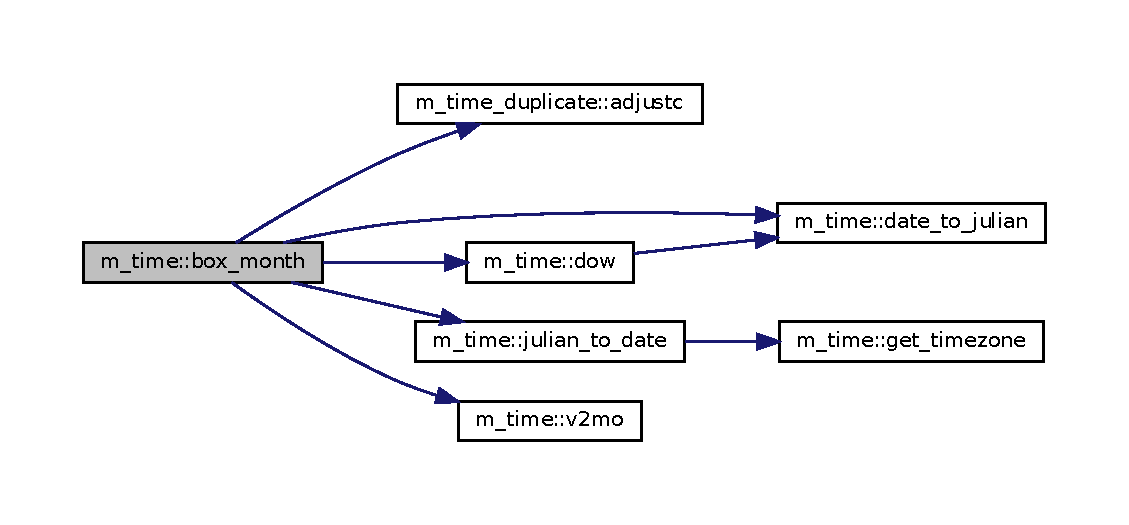
\includegraphics[width=350pt]{namespacem__time_a0fe7540912df30d3578f3c469413aea8_cgraph}
\end{center}
\end{figure}
\mbox{\Hypertarget{namespacem__time_af558bfc1fd5b13a6b879b3969866956f}\label{namespacem__time_af558bfc1fd5b13a6b879b3969866956f}} 
\index{m\_time@{m\_time}!call\_sleep@{call\_sleep}}
\index{call\_sleep@{call\_sleep}!m\_time@{m\_time}}
\doxysubsubsection{\texorpdfstring{call\_sleep()}{call\_sleep()}}
{\footnotesize\ttfamily subroutine, private m\+\_\+time\+::call\+\_\+sleep (\begin{DoxyParamCaption}\item[{integer(kind=c\+\_\+int), intent(in)}]{wait\+\_\+seconds }\end{DoxyParamCaption})\hspace{0.3cm}{\ttfamily [private]}}

Here is the caller graph for this function\+:\nopagebreak
\begin{figure}[H]
\begin{center}
\leavevmode
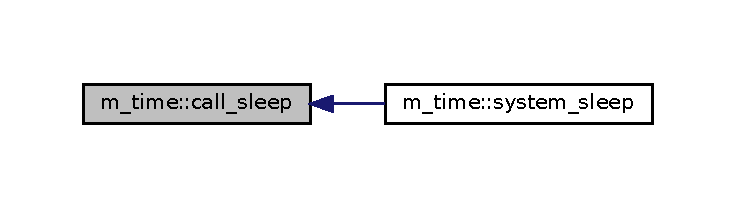
\includegraphics[width=350pt]{namespacem__time_af558bfc1fd5b13a6b879b3969866956f_icgraph}
\end{center}
\end{figure}
\mbox{\Hypertarget{namespacem__time_ae63783f7479d2f5093c8031d38ce4304}\label{namespacem__time_ae63783f7479d2f5093c8031d38ce4304}} 
\index{m\_time@{m\_time}!call\_usleep@{call\_usleep}}
\index{call\_usleep@{call\_usleep}!m\_time@{m\_time}}
\doxysubsubsection{\texorpdfstring{call\_usleep()}{call\_usleep()}}
{\footnotesize\ttfamily subroutine, private m\+\_\+time\+::call\+\_\+usleep (\begin{DoxyParamCaption}\item[{integer(kind=c\+\_\+int), intent(in)}]{wait\+\_\+seconds }\end{DoxyParamCaption})\hspace{0.3cm}{\ttfamily [private]}}

Here is the caller graph for this function\+:\nopagebreak
\begin{figure}[H]
\begin{center}
\leavevmode
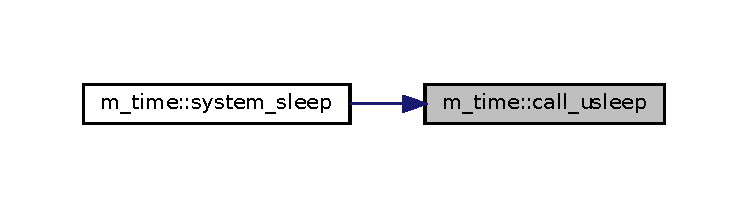
\includegraphics[width=350pt]{namespacem__time_ae63783f7479d2f5093c8031d38ce4304_icgraph}
\end{center}
\end{figure}
\mbox{\Hypertarget{namespacem__time_a3fccc53c2650104eff084c7998d18f54}\label{namespacem__time_a3fccc53c2650104eff084c7998d18f54}} 
\index{m\_time@{m\_time}!d2j@{d2j}}
\index{d2j@{d2j}!m\_time@{m\_time}}
\doxysubsubsection{\texorpdfstring{d2j()}{d2j()}}
{\footnotesize\ttfamily real(kind=\mbox{\hyperlink{namespacem__time_ac10ea9e8d59ec74eaa7d89f2517d7422}{realtime}}) function, public m\+\_\+time\+::d2j (\begin{DoxyParamCaption}\item[{integer, dimension(8), intent(in), optional}]{dat }\end{DoxyParamCaption})}

\hypertarget{namespacem__time_autotoc_md160}{}\doxysubsubsection{N\+A\+ME}\label{namespacem__time_autotoc_md160}
d2j(3f) -\/ \mbox{[}M\+\_\+time\+:J\+U\+L\+I\+AN\mbox{]} given D\+AT date-\/time array returns Julian Date (L\+I\+C\+E\+N\+SE\+:PD)\hypertarget{namespacem__time_autotoc_md161}{}\doxysubsubsection{S\+Y\+N\+O\+P\+S\+IS}\label{namespacem__time_autotoc_md161}
\begin{DoxyVerb}function d2j(dat) result (julian)

 integer,intent(in)  :: dat(8)
 real(kind=realtime) :: julian
\end{DoxyVerb}
\hypertarget{namespacem__time_autotoc_md162}{}\doxysubsubsection{D\+E\+S\+C\+R\+I\+P\+T\+I\+ON}\label{namespacem__time_autotoc_md162}
Given D\+AT date-\/time array returns Julian Date\hypertarget{namespacem__time_autotoc_md163}{}\doxysubsubsection{O\+P\+T\+I\+O\+NS}\label{namespacem__time_autotoc_md163}
dat Integer array holding a \char`\"{}\+D\+A\+T\char`\"{} array, similar in structure to the array returned by the intrinsic D\+A\+T\+E\+\_\+\+A\+N\+D\+\_\+\+T\+I\+M\+E(3f)\+:

dat=\mbox{[} year,month,day,timezone,hour,\& \& minutes,seconds,milliseconds\mbox{]}

If not present, use current time. \hypertarget{namespacem__time_autotoc_md164}{}\doxysubsubsection{R\+E\+T\+U\+R\+NS}\label{namespacem__time_autotoc_md164}
julian The Julian Date.\hypertarget{namespacem__time_autotoc_md165}{}\doxysubsubsection{E\+X\+A\+M\+P\+LE}\label{namespacem__time_autotoc_md165}
\begin{DoxyVerb}Sample program:

 program demo_d2j
 use M_time, only : d2j
 implicit none
 integer :: dat(8)
    call date_and_time(values=dat)
    write(*,'(" Today is:",*(i0:,":"))')dat
    write(*,*)'Julian Date is ',d2j(dat)
 end program demo_d2j

results:

 Today is:2016:7:19:-240:2:11:50:885
 Julian Date is    2457588.7582278359
\end{DoxyVerb}
\hypertarget{namespacem__time_autotoc_md166}{}\doxysubsubsection{A\+U\+T\+H\+OR}\label{namespacem__time_autotoc_md166}
John S. Urban, 2015 \hypertarget{namespacem__time_autotoc_md167}{}\doxysubsubsection{L\+I\+C\+E\+N\+SE}\label{namespacem__time_autotoc_md167}
Public Domain 

References date\+\_\+to\+\_\+julian().

Here is the call graph for this function\+:\nopagebreak
\begin{figure}[H]
\begin{center}
\leavevmode
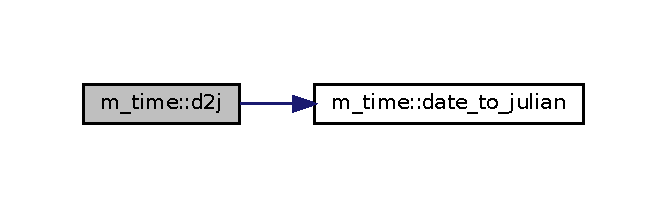
\includegraphics[width=320pt]{namespacem__time_a3fccc53c2650104eff084c7998d18f54_cgraph}
\end{center}
\end{figure}
Here is the caller graph for this function\+:\nopagebreak
\begin{figure}[H]
\begin{center}
\leavevmode
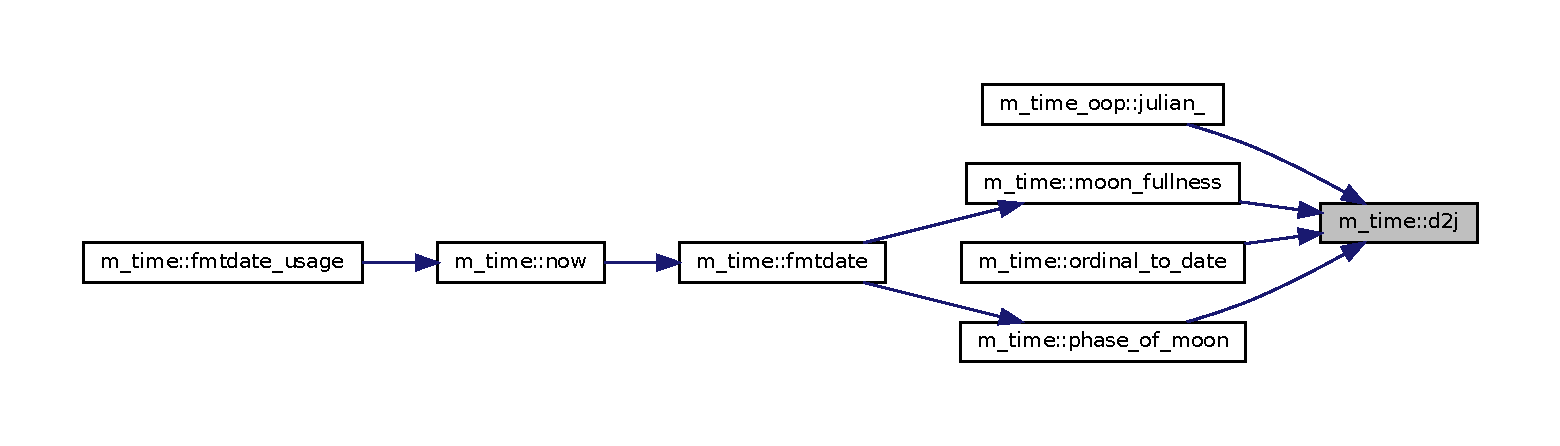
\includegraphics[width=350pt]{namespacem__time_a3fccc53c2650104eff084c7998d18f54_icgraph}
\end{center}
\end{figure}
\mbox{\Hypertarget{namespacem__time_a727dd77bbd4a5d0e3947c5d303845947}\label{namespacem__time_a727dd77bbd4a5d0e3947c5d303845947}} 
\index{m\_time@{m\_time}!d2o@{d2o}}
\index{d2o@{d2o}!m\_time@{m\_time}}
\doxysubsubsection{\texorpdfstring{d2o()}{d2o()}}
{\footnotesize\ttfamily integer function, public m\+\_\+time\+::d2o (\begin{DoxyParamCaption}\item[{integer, dimension(8), intent(in), optional}]{dat }\end{DoxyParamCaption})}

\hypertarget{namespacem__time_autotoc_md34}{}\doxysubsubsection{N\+A\+ME}\label{namespacem__time_autotoc_md34}
d2o(3f) -\/ \mbox{[}M\+\_\+time\+:O\+R\+D\+I\+N\+A\+L\+\_\+\+D\+AY\mbox{]} converts D\+AT date-\/time array to Ordinal day (L\+I\+C\+E\+N\+SE\+:PD)\hypertarget{namespacem__time_autotoc_md35}{}\doxysubsubsection{S\+Y\+N\+O\+P\+S\+IS}\label{namespacem__time_autotoc_md35}
\begin{DoxyVerb}function d2o(dat) result (ordinal)

 integer,intent(in),optional :: dat(8)
 integer                     :: ordinal
\end{DoxyVerb}
\hypertarget{namespacem__time_autotoc_md36}{}\doxysubsubsection{D\+E\+S\+C\+R\+I\+P\+T\+I\+ON}\label{namespacem__time_autotoc_md36}
Given a date in the form of a \char`\"{}\+D\+A\+T\char`\"{} array return the Ordinal Day, (ie. \char`\"{}the day of the year\char`\"{}).\hypertarget{namespacem__time_autotoc_md37}{}\doxysubsubsection{O\+P\+T\+I\+O\+NS}\label{namespacem__time_autotoc_md37}
dat Integer array holding a \char`\"{}\+D\+A\+T\char`\"{} array, similar in structure to the array returned by the intrinsic D\+A\+T\+E\+\_\+\+A\+N\+D\+\_\+\+T\+I\+M\+E(3f)\+: \begin{DoxyVerb}dat=[ year,month,day,timezone,hour,&
 & minutes,seconds,milliseconds]
\end{DoxyVerb}
 \hypertarget{namespacem__time_autotoc_md38}{}\doxysubsubsection{R\+E\+T\+U\+R\+NS}\label{namespacem__time_autotoc_md38}
ordinal The day of the year calculated for the given input date, where Jan 1st=1.\hypertarget{namespacem__time_autotoc_md39}{}\doxysubsubsection{E\+X\+A\+M\+P\+LE}\label{namespacem__time_autotoc_md39}
\begin{DoxyVerb}Sample program:

 program demo_d2o
 use M_time, only : d2o
 implicit none
 integer :: dat(8)
    call date_and_time(values=dat)
    write(*,'(" Today is:",*(i0:,":"))')dat
    write(*,*)'Day of year is:',d2o(dat)

    ! year,month,day,timezone,hour,minute,seconds,milliseconds
    dat=[2020,12,31,-240,12,0,0,0]
    write(*,*)dat(1),' Days in year is:',d2o(dat)

    dat=[2021,12,31,-240,12,0,0,0]
    write(*,*)dat(1),' Days in year is:',d2o(dat)

    dat=[2022,12,31,-240,12,0,0,0]
    write(*,*)dat(1),' Days in year is:',d2o(dat)

    dat=[2023,12,31,-240,12,0,0,0]
    write(*,*)dat(1),' Days in year is:',d2o(dat)

    dat=[2024,12,31,-240,12,0,0,0]
    write(*,*)dat(1),' Days in year is:',d2o(dat)

 end program demo_d2o

results:

 Today is:2016:7:19:-240:20:1:19:829
 Day of year is:         201
        2020  Days in year is:         366
        2021  Days in year is:         365
        2022  Days in year is:         365
        2023  Days in year is:         365
        2024  Days in year is:         366
\end{DoxyVerb}
\hypertarget{namespacem__time_autotoc_md40}{}\doxysubsubsection{A\+U\+T\+H\+OR}\label{namespacem__time_autotoc_md40}
John S. Urban, 2015 \hypertarget{namespacem__time_autotoc_md41}{}\doxysubsubsection{L\+I\+C\+E\+N\+SE}\label{namespacem__time_autotoc_md41}
Public Domain 

References date\+\_\+to\+\_\+unix(), secday, and m\+\_\+time\+\_\+duplicate\+::stderr().

Here is the call graph for this function\+:\nopagebreak
\begin{figure}[H]
\begin{center}
\leavevmode
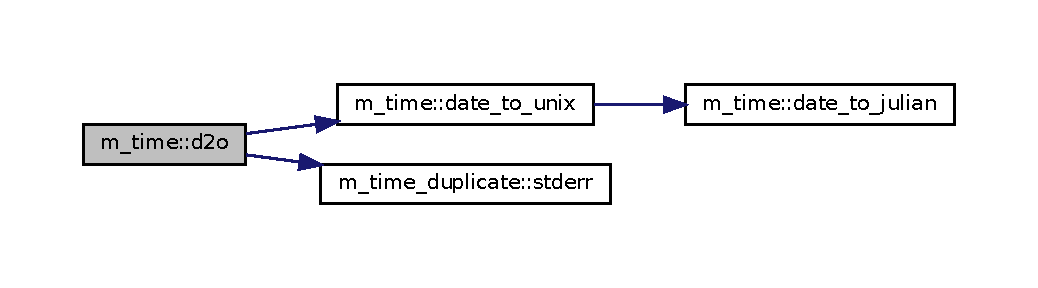
\includegraphics[width=350pt]{namespacem__time_a727dd77bbd4a5d0e3947c5d303845947_cgraph}
\end{center}
\end{figure}
Here is the caller graph for this function\+:\nopagebreak
\begin{figure}[H]
\begin{center}
\leavevmode
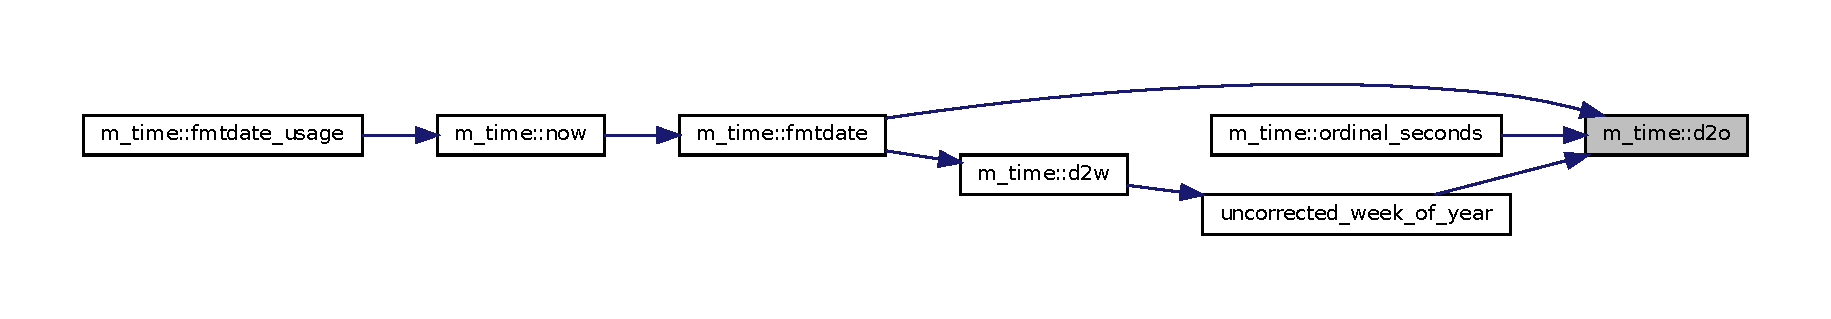
\includegraphics[width=350pt]{namespacem__time_a727dd77bbd4a5d0e3947c5d303845947_icgraph}
\end{center}
\end{figure}
\mbox{\Hypertarget{namespacem__time_a1506e2889a156387df4481ed0534be81}\label{namespacem__time_a1506e2889a156387df4481ed0534be81}} 
\index{m\_time@{m\_time}!d2u@{d2u}}
\index{d2u@{d2u}!m\_time@{m\_time}}
\doxysubsubsection{\texorpdfstring{d2u()}{d2u()}}
{\footnotesize\ttfamily real(kind=\mbox{\hyperlink{namespacem__time_ac10ea9e8d59ec74eaa7d89f2517d7422}{realtime}}) function, public m\+\_\+time\+::d2u (\begin{DoxyParamCaption}\item[{integer, dimension(8), intent(in), optional}]{dat }\end{DoxyParamCaption})}

\hypertarget{namespacem__time_autotoc_md176}{}\doxysubsubsection{N\+A\+ME}\label{namespacem__time_autotoc_md176}
d2u(3f) -\/ \mbox{[}M\+\_\+time\+:U\+N\+I\+X\+\_\+\+E\+P\+O\+CH\mbox{]} given D\+AT date-\/time array returns Unix Epoch Time (U\+ET starts at 0000 on 1 Jan. 1970, U\+TC) (L\+I\+C\+E\+N\+SE\+:PD)\hypertarget{namespacem__time_autotoc_md177}{}\doxysubsubsection{S\+Y\+N\+O\+P\+S\+IS}\label{namespacem__time_autotoc_md177}
\begin{DoxyVerb}function d2u(dat) result (unixtime)

   integer,intent(in),optional :: dat(8)
   real(kind=realtime)         :: unixtime
\end{DoxyVerb}
\hypertarget{namespacem__time_autotoc_md178}{}\doxysubsubsection{D\+E\+S\+C\+R\+I\+P\+T\+I\+ON}\label{namespacem__time_autotoc_md178}
Converts a D\+AT date-\/time array to a Unix Epoch Time value. Typically mathematical operations such as sums, sorting and comparison are performed with simple U\+ET numeric values, and then they are converted back.\hypertarget{namespacem__time_autotoc_md179}{}\doxysubsubsection{O\+P\+T\+I\+O\+NS}\label{namespacem__time_autotoc_md179}
dat Integer array holding a \char`\"{}\+D\+A\+T\char`\"{} array, similar in structure to the array returned by the intrinsic D\+A\+T\+E\+\_\+\+A\+N\+D\+\_\+\+T\+I\+M\+E(3f)\+: \begin{DoxyVerb}   dat=[ year,month,day,timezone,hour,&
    & minutes,seconds,milliseconds]
\end{DoxyVerb}


If not present the current time is used\hypertarget{namespacem__time_autotoc_md180}{}\doxysubsubsection{R\+E\+T\+U\+R\+NS}\label{namespacem__time_autotoc_md180}
unixtime The \char`\"{}\+Unix Epoch\char`\"{} time, or the number of seconds since 00\+:00\+:00 on January 1st, 1970, U\+TC.\hypertarget{namespacem__time_autotoc_md181}{}\doxysubsubsection{E\+X\+A\+M\+P\+LE}\label{namespacem__time_autotoc_md181}
\begin{DoxyVerb}Sample program:

 program demo_d2u
 use M_time, only : d2u
 implicit none
 integer           :: dat(8)
    call date_and_time(values=dat)
    write(*,'(" Today is:",*(i0:,":"))')dat
    write(*,*)'Unix Epoch time is ',d2u(dat)
 end program demo_d2u

results:

 Today is:2016:7:19:-240:2:0:48:561
 Unix Epoch time is    1468908048.5610321
\end{DoxyVerb}
 \hypertarget{namespacem__time_autotoc_md182}{}\doxysubsubsection{A\+U\+T\+H\+OR}\label{namespacem__time_autotoc_md182}
John S. Urban, 2015 \hypertarget{namespacem__time_autotoc_md183}{}\doxysubsubsection{L\+I\+C\+E\+N\+SE}\label{namespacem__time_autotoc_md183}
Public Domain 

References date\+\_\+to\+\_\+unix().

Here is the call graph for this function\+:\nopagebreak
\begin{figure}[H]
\begin{center}
\leavevmode
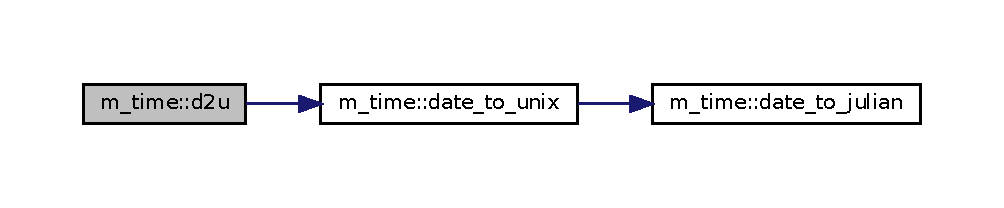
\includegraphics[width=350pt]{namespacem__time_a1506e2889a156387df4481ed0534be81_cgraph}
\end{center}
\end{figure}
Here is the caller graph for this function\+:\nopagebreak
\begin{figure}[H]
\begin{center}
\leavevmode
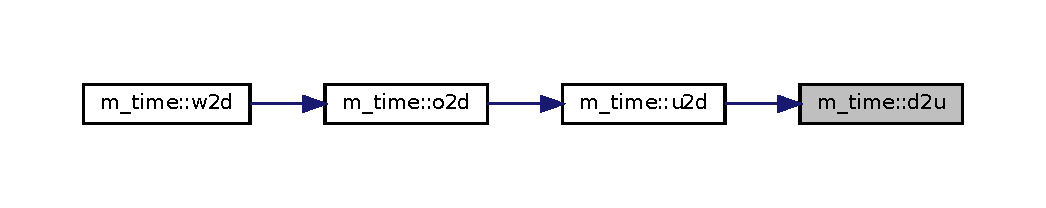
\includegraphics[width=350pt]{namespacem__time_a1506e2889a156387df4481ed0534be81_icgraph}
\end{center}
\end{figure}
\mbox{\Hypertarget{namespacem__time_ad4ff99ad6f6d5282c4b65ad636a2a627}\label{namespacem__time_ad4ff99ad6f6d5282c4b65ad636a2a627}} 
\index{m\_time@{m\_time}!d2w@{d2w}}
\index{d2w@{d2w}!m\_time@{m\_time}}
\doxysubsubsection{\texorpdfstring{d2w()}{d2w()}}
{\footnotesize\ttfamily subroutine, public m\+\_\+time\+::d2w (\begin{DoxyParamCaption}\item[{integer, dimension(8), intent(in)}]{dat,  }\item[{integer, intent(out)}]{iso\+\_\+year,  }\item[{integer, intent(out)}]{iso\+\_\+week,  }\item[{integer, intent(out)}]{iso\+\_\+weekday,  }\item[{character(len=10), intent(out)}]{iso\+\_\+name }\end{DoxyParamCaption})}

\hypertarget{namespacem__time_autotoc_md123}{}\doxysubsubsection{N\+A\+ME}\label{namespacem__time_autotoc_md123}
d2w(3f) -\/ \mbox{[}M\+\_\+time\+:W\+E\+E\+K\+\_\+\+O\+F\+\_\+\+Y\+E\+AR\mbox{]} calculate iso-\/8601 Week-\/numbering year date yyyy-\/\+Www-\/d given D\+AT date-\/time array (L\+I\+C\+E\+N\+SE\+:PD)\hypertarget{namespacem__time_autotoc_md124}{}\doxysubsubsection{S\+Y\+N\+O\+P\+S\+IS}\label{namespacem__time_autotoc_md124}
\begin{DoxyVerb}subroutine d2w(dat,iso_year,iso_week,iso_weekday,iso_name)

 integer,intent(in)              :: dat(8)     ! input date array
 integer,intent(out)             :: iso_year, iso_week, iso_weekday
 character(len=10),intent(out)   :: iso_name
\end{DoxyVerb}
\hypertarget{namespacem__time_autotoc_md125}{}\doxysubsubsection{D\+E\+S\+C\+R\+I\+P\+T\+I\+ON}\label{namespacem__time_autotoc_md125}
Given a \char`\"{}\+D\+A\+T\char`\"{} array defining a date and time, return the I\+S\+O-\/8601 Week in two formats -- as three integer values defining the I\+SO year, week of year and weekday; and as a string of the form \char`\"{}yyyy-\/\+Www-\/d\char`\"{}.\hypertarget{namespacem__time_autotoc_md126}{}\doxysubsubsection{O\+P\+T\+I\+O\+NS}\label{namespacem__time_autotoc_md126}
dat \char`\"{}\+D\+A\+T\char`\"{} array (an integer array of the same format as the array returned by the intrinsic D\+A\+T\+E\+\_\+\+A\+N\+D\+\_\+\+T\+I\+M\+E(3f)) describing the date, which is the basic time description used by the other M\+\_\+time(3fm) module procedures. \hypertarget{namespacem__time_autotoc_md127}{}\doxysubsubsection{R\+E\+T\+U\+R\+NS}\label{namespacem__time_autotoc_md127}
iso\+\_\+year I\+S\+O-\/8601 year number for the given date iso\+\_\+week I\+S\+O-\/8601 week number for the given date iso\+\_\+weekday I\+S\+O-\/8601 weekday number for the given date iso\+\_\+name I\+S\+O-\/8601 Week string for the data in the form \char`\"{}yyyy-\/\+Www-\/d\char`\"{}.\hypertarget{namespacem__time_autotoc_md128}{}\doxysubsubsection{E\+X\+A\+M\+P\+LE}\label{namespacem__time_autotoc_md128}
\begin{DoxyVerb}Sample program:

 program demo_d2w
 use M_time, only : d2w
 implicit none
 integer           :: dat(8)     ! input date array
 integer           :: iso_year, iso_week, iso_weekday
 character(len=10) :: iso_name
    call date_and_time(values=dat)
    call d2w(dat,iso_year,iso_week,iso_weekday,iso_name)
    write(*,'("ISO-8601 Week:   ",a)')iso_name
    write(*,'(a,i0)')'ISO-8601 year    ',iso_year
    write(*,'(a,i0)')'ISO-8601 week    ',iso_week
    write(*,'(a,i0)')'ISO-8601 weekday ',iso_weekday
 end program demo_d2w

results:

 ISO-8601 Week:   2016-W29-1
 ISO-8601 year    2016
 ISO-8601 week    29
 ISO-8601 weekday 1
\end{DoxyVerb}
\hypertarget{namespacem__time_autotoc_md129}{}\doxysubsubsection{D\+E\+F\+I\+N\+I\+T\+I\+ON}\label{namespacem__time_autotoc_md129}
The I\+S\+O-\/8601 date and time standard was issued by the International Organization for Standardization (I\+SO). It is used (mainly) in government and business for fiscal years, as well as in timekeeping. The system specifies a week year atop the Gregorian calendar by defining a notation for ordinal weeks of the year.

An I\+SO week-\/numbering year (also called I\+SO year informally) has 52 or 53 full weeks. That is 364 or 371 days instead of the usual 365 or 366 days. The extra week is referred to here as a leap week, although I\+S\+O-\/8601 does not use this term. Weeks start with Monday. The first week of a year is the week that contains the first Thursday of the year (and, hence, always contains 4 January). I\+SO week year numbering therefore slightly deviates from the Gregorian for some days close to January 1st.\hypertarget{namespacem__time_autotoc_md130}{}\doxysubsubsection{C\+A\+L\+C\+U\+L\+A\+T\+I\+ON}\label{namespacem__time_autotoc_md130}
The I\+S\+O-\/8601 week number of any date can be calculated, given its ordinal date (i.\+e. position within the year) and its day of the week.\hypertarget{namespacem__time_autotoc_md131}{}\doxysubsubsection{M\+E\+T\+H\+OD}\label{namespacem__time_autotoc_md131}
Using I\+SO weekday numbers (running from 1 for Monday to 7 for Sunday), subtract the weekday from the ordinal date, then add 10. Divide the result by 7. Ignore the remainder; the quotient equals the week number. If the week number thus obtained equals 0, it means that the given date belongs to the preceding (week-\/based) year. If a week number of 53 is obtained, one must check that the date is not actually in week 1 of the following year.

These two statements are assumed true when correcting the dates around January 1st\+:

o The number of weeks in a given year is equal to the corresponding week number of 28 December. o January 4th is always in the first week.\hypertarget{namespacem__time_autotoc_md132}{}\doxysubsubsection{I\+S\+O\+\_\+\+N\+A\+ME}\label{namespacem__time_autotoc_md132}
Week date representations are in the format Y\+Y\+Y\+Y\+Www-\/D.

o \mbox{[}Y\+Y\+YY\mbox{]} indicates the I\+SO week-\/numbering year which is slightly different from the traditional Gregorian calendar year. o \mbox{[}Www\mbox{]} is the week number prefixed by the letter W, from W01 through W53. o \mbox{[}D\mbox{]} is the weekday number, from 1 through 7, beginning with Monday and ending with Sunday.

For example, the Gregorian date 31 December 2006 corresponds to the Sunday of the 52nd week of 2006, and is written

2006-\/W52-\/7 (extended form) or 2006W527 (compact form).\hypertarget{namespacem__time_autotoc_md133}{}\doxysubsubsection{R\+E\+F\+E\+R\+E\+N\+CE}\label{namespacem__time_autotoc_md133}
From Wikipedia, the free encyclopedia 2015-\/12-\/19\hypertarget{namespacem__time_autotoc_md134}{}\doxysubsubsection{A\+U\+T\+H\+OR}\label{namespacem__time_autotoc_md134}
John S. Urban, 2015-\/12-\/19 \hypertarget{namespacem__time_autotoc_md135}{}\doxysubsubsection{L\+I\+C\+E\+N\+SE}\label{namespacem__time_autotoc_md135}
Public Domain 

References uncorrected\+\_\+week\+\_\+of\+\_\+year().

Here is the call graph for this function\+:\nopagebreak
\begin{figure}[H]
\begin{center}
\leavevmode
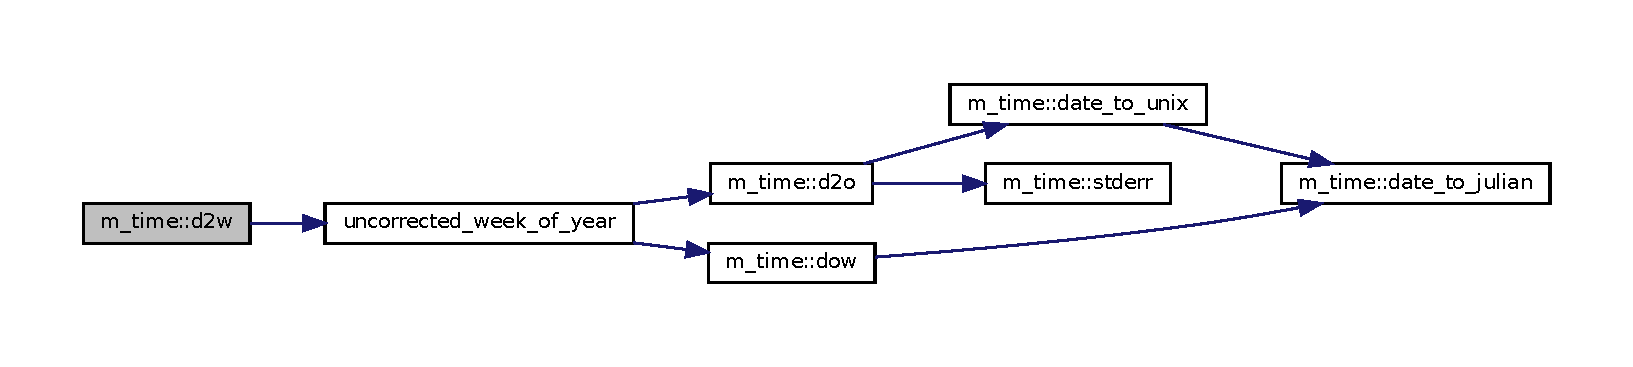
\includegraphics[width=350pt]{namespacem__time_ad4ff99ad6f6d5282c4b65ad636a2a627_cgraph}
\end{center}
\end{figure}
Here is the caller graph for this function\+:\nopagebreak
\begin{figure}[H]
\begin{center}
\leavevmode
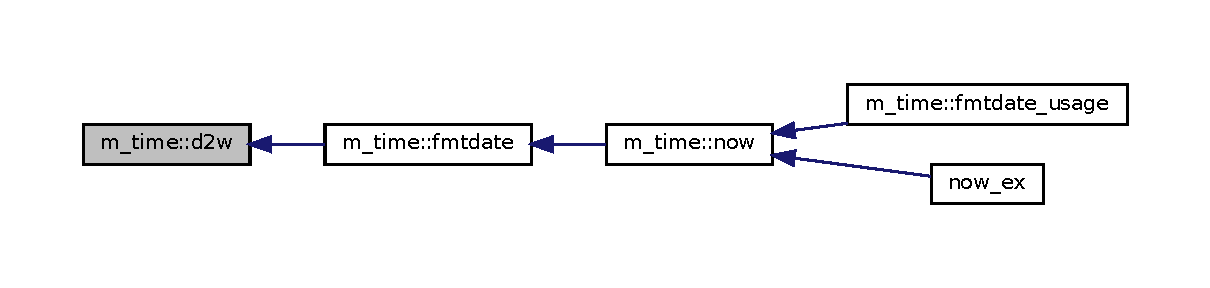
\includegraphics[width=350pt]{namespacem__time_ad4ff99ad6f6d5282c4b65ad636a2a627_icgraph}
\end{center}
\end{figure}
\mbox{\Hypertarget{namespacem__time_acfdc970b4154b0c15bd33727636e3992}\label{namespacem__time_acfdc970b4154b0c15bd33727636e3992}} 
\index{m\_time@{m\_time}!date\_to\_julian@{date\_to\_julian}}
\index{date\_to\_julian@{date\_to\_julian}!m\_time@{m\_time}}
\doxysubsubsection{\texorpdfstring{date\_to\_julian()}{date\_to\_julian()}}
{\footnotesize\ttfamily subroutine, public m\+\_\+time\+::date\+\_\+to\+\_\+julian (\begin{DoxyParamCaption}\item[{integer, dimension(8), intent(in)}]{dat,  }\item[{real(kind=\mbox{\hyperlink{namespacem__time_ac10ea9e8d59ec74eaa7d89f2517d7422}{realtime}}), intent(out)}]{julian,  }\item[{integer, intent(out)}]{ierr }\end{DoxyParamCaption})}

\hypertarget{namespacem__time_autotoc_md0}{}\doxysubsubsection{N\+A\+ME}\label{namespacem__time_autotoc_md0}
date\+\_\+to\+\_\+julian(3f) -\/ \mbox{[}M\+\_\+time\+:J\+U\+L\+I\+AN\mbox{]} converts D\+AT date-\/time array to Julian Date (L\+I\+C\+E\+N\+SE\+:PD)\hypertarget{namespacem__time_autotoc_md1}{}\doxysubsubsection{S\+Y\+N\+O\+P\+S\+IS}\label{namespacem__time_autotoc_md1}
\begin{DoxyVerb}subroutine date_to_julian(dat,juliandate,ierr)

 integer,intent(in)               :: dat(8)
 real(kind=realtime),intent(out)  :: juliandate
 integer,intent(out)              :: ierr
\end{DoxyVerb}
\hypertarget{namespacem__time_autotoc_md2}{}\doxysubsubsection{D\+E\+S\+C\+R\+I\+P\+T\+I\+ON}\label{namespacem__time_autotoc_md2}
Converts a D\+AT date-\/time array to a Unix Epoch Time (U\+ET) value. U\+ET is the number of seconds since 00\+:00 on January 1st, 1970, U\+TC.\hypertarget{namespacem__time_autotoc_md3}{}\doxysubsubsection{O\+P\+T\+I\+O\+NS}\label{namespacem__time_autotoc_md3}
dat Integer array holding a \char`\"{}\+D\+A\+T\char`\"{} array, similar in structure to the array returned by the intrinsic D\+A\+T\+E\+\_\+\+A\+N\+D\+\_\+\+T\+I\+M\+E(3f)\+:

dat=\mbox{[} year,month,day,timezone,hour,\& \& minutes,seconds,milliseconds\mbox{]}\hypertarget{namespacem__time_autotoc_md4}{}\doxysubsubsection{R\+E\+T\+U\+R\+NS}\label{namespacem__time_autotoc_md4}
juliandate A Julian Ephemeris Date (J\+ED) is the number of days since noon (not midnight) on January 1st, 4713 BC. ierr Error code. If 0 no error occurred.\hypertarget{namespacem__time_autotoc_md5}{}\doxysubsubsection{E\+X\+A\+M\+P\+LE}\label{namespacem__time_autotoc_md5}
\begin{DoxyVerb}Sample Program:

 program demo_date_to_julian
 use M_time, only : date_to_julian,realtime
 implicit none
 integer             :: dat(8)
 real(kind=realtime) :: juliandate
 integer             :: ierr
    ! generate DAT array
    call date_and_time(values=dat)
    ! show DAT array
    write(*,'(" Today is:",*(i0:,":"))')dat
    ! convert DAT to Julian Date
    call date_to_julian(dat,juliandate,ierr)
    write(*,*)'Julian Date is ',juliandate
    write(*,*)'ierr is ',ierr
 end program demo_date_to_julian

results:

 Today is:2016:7:19:-240:11:3:13:821
 Julian Date is    2457589.1272432986
 ierr is            0
\end{DoxyVerb}
\hypertarget{namespacem__time_autotoc_md6}{}\doxysubsubsection{A\+U\+T\+H\+OR}\label{namespacem__time_autotoc_md6}
John S. Urban, 2015 \hypertarget{namespacem__time_autotoc_md7}{}\doxysubsubsection{L\+I\+C\+E\+N\+SE}\label{namespacem__time_autotoc_md7}
Public Domain
\begin{DoxyParams}[1]{Parameters}
\mbox{\texttt{ in}}  & {\em dat} & A\+U\+T\+H\+OR\+: John S. Urban \\
\hline
\end{DoxyParams}
\hypertarget{namespacem__time_autotoc_md9}{}\doxysubsubsection{V\+E\+R\+S\+I\+O\+N\+:   2.\+0 2022-\/01-\/16}\label{namespacem__time_autotoc_md9}
R\+E\+F\+E\+R\+E\+N\+CE\+: From Wikipedia, the free encyclopedia 2015-\/12-\/19 Here is the caller graph for this function\+:\nopagebreak
\begin{figure}[H]
\begin{center}
\leavevmode
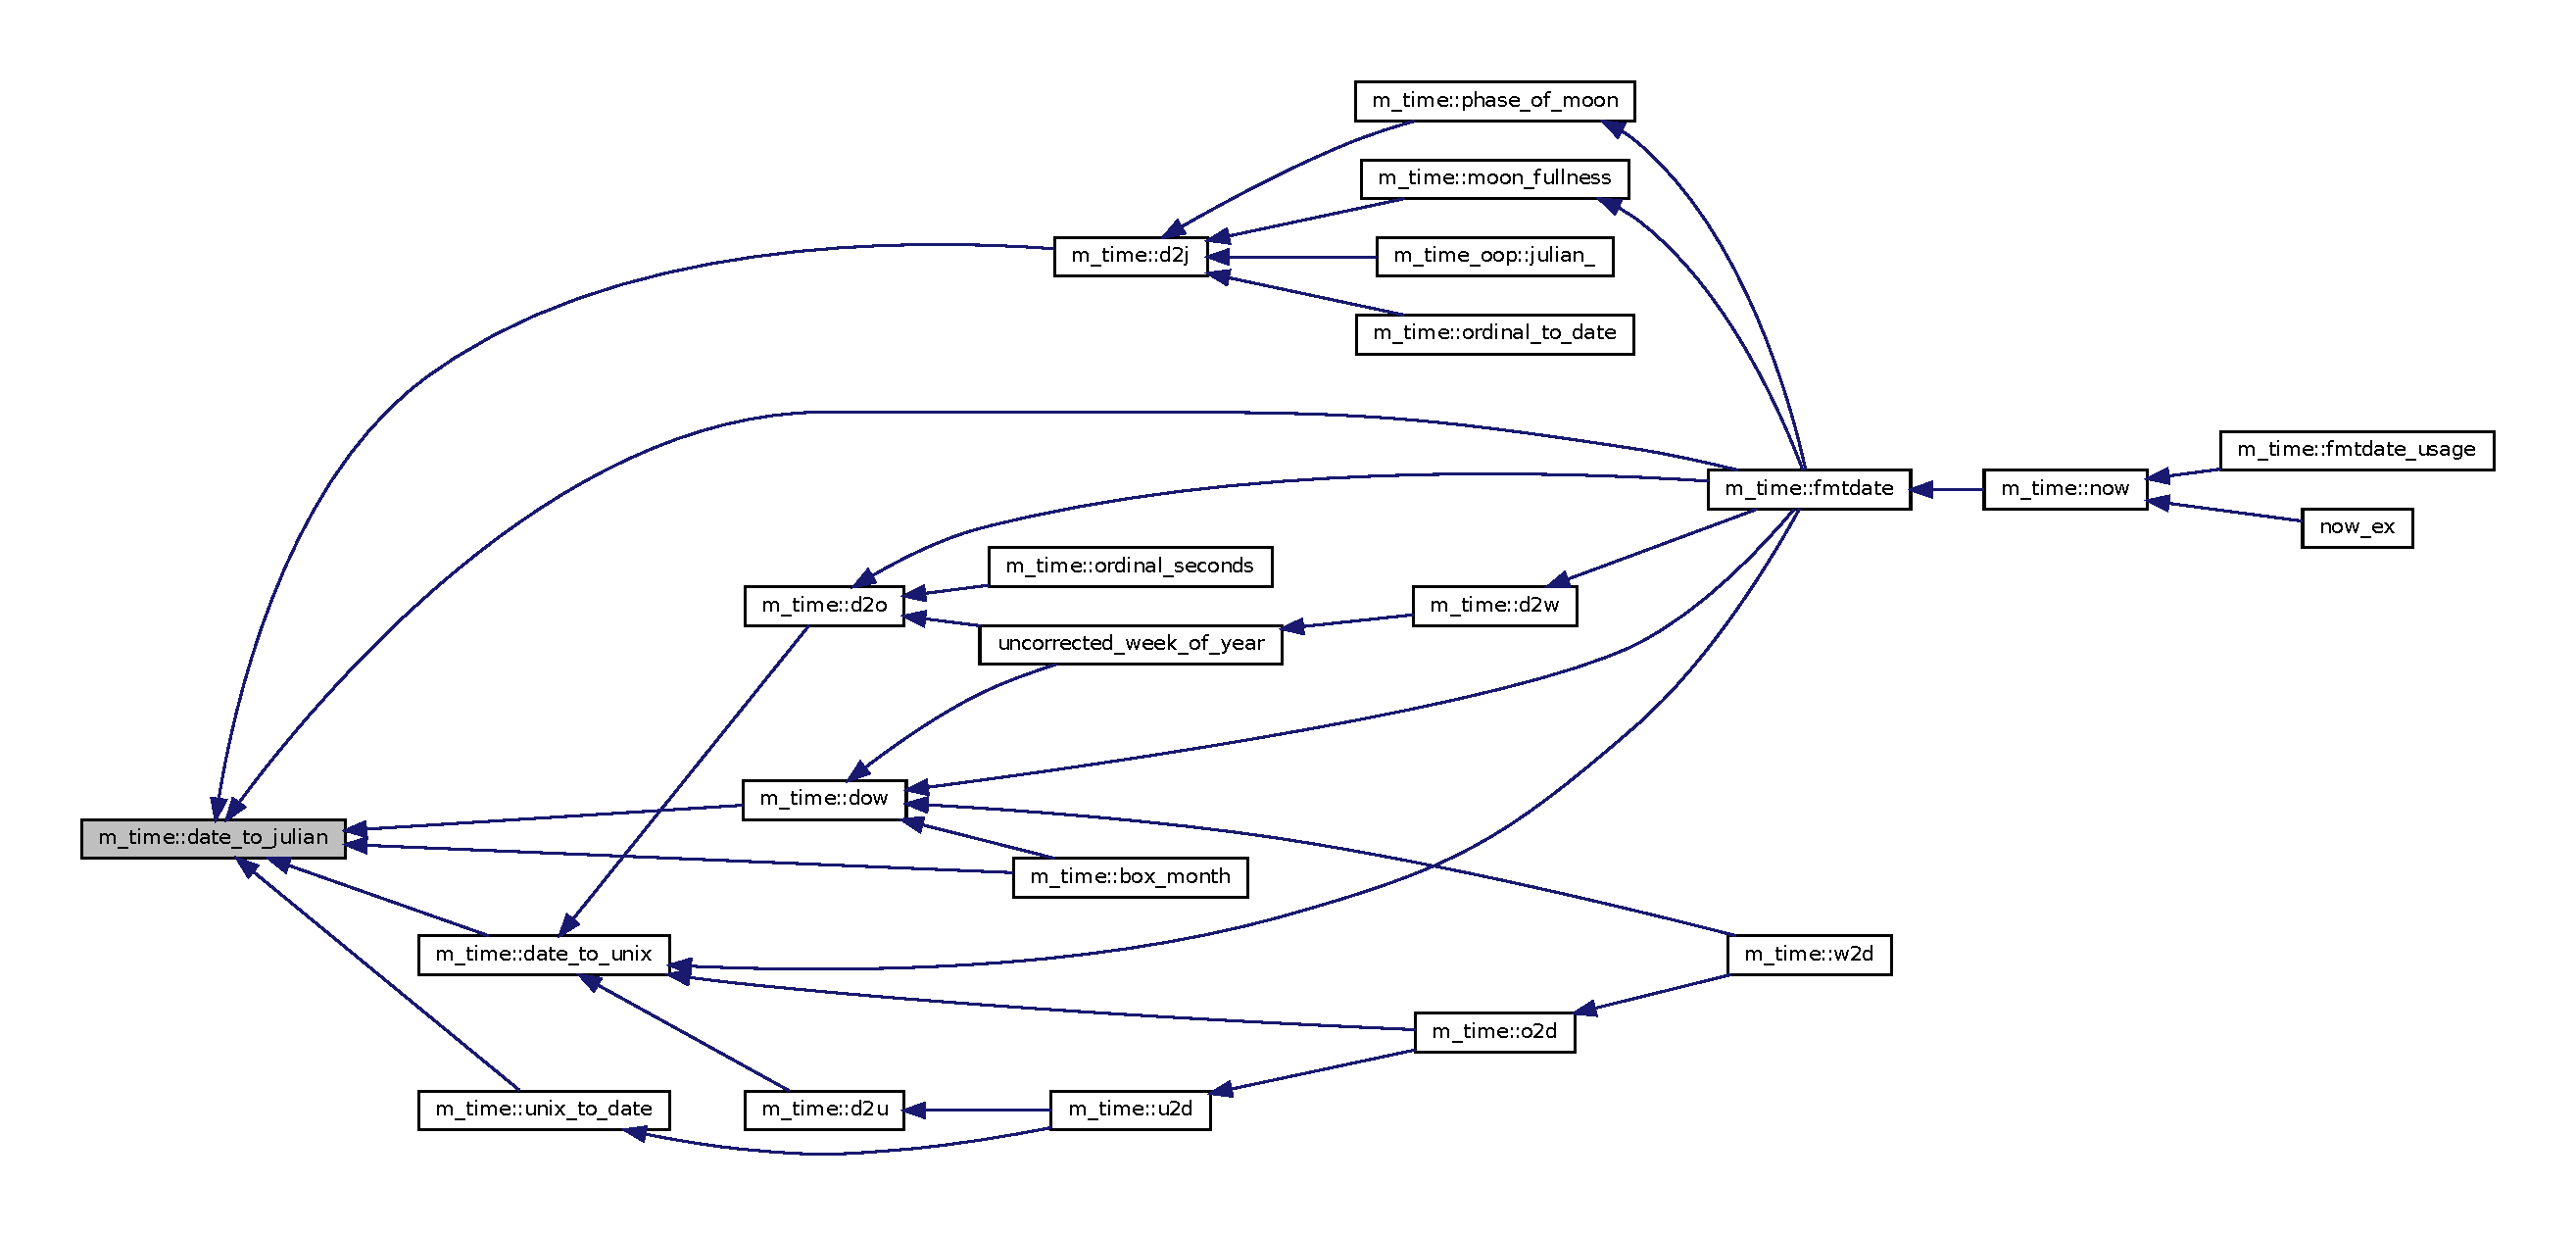
\includegraphics[width=350pt]{namespacem__time_acfdc970b4154b0c15bd33727636e3992_icgraph}
\end{center}
\end{figure}
\mbox{\Hypertarget{namespacem__time_aed245c691853279ebf0ce899dec9caa9}\label{namespacem__time_aed245c691853279ebf0ce899dec9caa9}} 
\index{m\_time@{m\_time}!date\_to\_unix@{date\_to\_unix}}
\index{date\_to\_unix@{date\_to\_unix}!m\_time@{m\_time}}
\doxysubsubsection{\texorpdfstring{date\_to\_unix()}{date\_to\_unix()}}
{\footnotesize\ttfamily subroutine, public m\+\_\+time\+::date\+\_\+to\+\_\+unix (\begin{DoxyParamCaption}\item[{integer, dimension(8), intent(in)}]{dat,  }\item[{real(kind=\mbox{\hyperlink{namespacem__time_ac10ea9e8d59ec74eaa7d89f2517d7422}{realtime}}), intent(out)}]{unixtime,  }\item[{integer, intent(out)}]{ierr }\end{DoxyParamCaption})}

\hypertarget{namespacem__time_autotoc_md18}{}\doxysubsubsection{N\+A\+ME}\label{namespacem__time_autotoc_md18}
date\+\_\+to\+\_\+unix(3f) -\/ \mbox{[}M\+\_\+time\+:U\+N\+I\+X\+\_\+\+E\+P\+O\+CH\mbox{]} converts D\+AT date-\/time array to Unix Epoch Time (L\+I\+C\+E\+N\+SE\+:PD)\hypertarget{namespacem__time_autotoc_md19}{}\doxysubsubsection{S\+Y\+N\+O\+P\+S\+IS}\label{namespacem__time_autotoc_md19}
\begin{DoxyVerb}subroutine date_to_unix(dat,unixtime,ierr)

 integer,intent(in)               :: dat(8)
 real(kind=realtime),intent(out)  :: unixtime
 integer,intent(out)              :: ierr
\end{DoxyVerb}
\hypertarget{namespacem__time_autotoc_md20}{}\doxysubsubsection{D\+E\+S\+C\+R\+I\+P\+T\+I\+ON}\label{namespacem__time_autotoc_md20}
Converts a D\+AT date-\/time array to a U\+ET (Unix Epoch Time).\hypertarget{namespacem__time_autotoc_md21}{}\doxysubsubsection{O\+P\+T\+I\+O\+NS}\label{namespacem__time_autotoc_md21}
dat Integer array holding a \char`\"{}\+D\+A\+T\char`\"{} array, similar in structure to the array returned by the intrinsic D\+A\+T\+E\+\_\+\+A\+N\+D\+\_\+\+T\+I\+M\+E(3f)\+: \begin{DoxyVerb}dat=[ year,month,day,timezone,hour,&
 & minutes,seconds,milliseconds]
\end{DoxyVerb}
 \hypertarget{namespacem__time_autotoc_md22}{}\doxysubsubsection{R\+E\+T\+U\+R\+NS}\label{namespacem__time_autotoc_md22}
unixtime The \char`\"{}\+Unix Epoch\char`\"{} time, or the number of seconds since 00\+:00\+:00 on January 1st, 1970, U\+TC. ierr Error code. If 0 no error occurred.\hypertarget{namespacem__time_autotoc_md23}{}\doxysubsubsection{E\+X\+A\+M\+P\+LE}\label{namespacem__time_autotoc_md23}
\begin{DoxyVerb} Sample program:

  program demo_date_to_unix
  use M_time, only : date_to_unix, realtime
  implicit none
  integer             :: dat(8)
  real(kind=realtime) :: unixtime
  integer             :: ierr
     call date_and_time(values=dat)
     write(*,'(" Today is:",*(i0:,":"))')dat
     call date_to_unix(dat,unixtime,ierr)
     write(*,*)'Unix Epoch time is ',unixtime
     write(*,*)'ierr is ',ierr
  end program demo_date_to_unix

 results:

  Today is:2016:7:18:-240:23:44:20:434
  Unix Epoch time is    1468899860.4340105
  ierr is            0
\end{DoxyVerb}
 \hypertarget{namespacem__time_autotoc_md24}{}\doxysubsubsection{A\+U\+T\+H\+OR}\label{namespacem__time_autotoc_md24}
John S. Urban, 2015 \hypertarget{namespacem__time_autotoc_md25}{}\doxysubsubsection{L\+I\+C\+E\+N\+SE}\label{namespacem__time_autotoc_md25}
Public Domain 

References date\+\_\+to\+\_\+julian(), and secday.

Here is the call graph for this function\+:\nopagebreak
\begin{figure}[H]
\begin{center}
\leavevmode
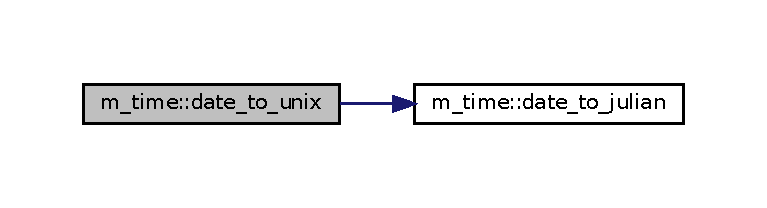
\includegraphics[width=350pt]{namespacem__time_aed245c691853279ebf0ce899dec9caa9_cgraph}
\end{center}
\end{figure}
Here is the caller graph for this function\+:\nopagebreak
\begin{figure}[H]
\begin{center}
\leavevmode
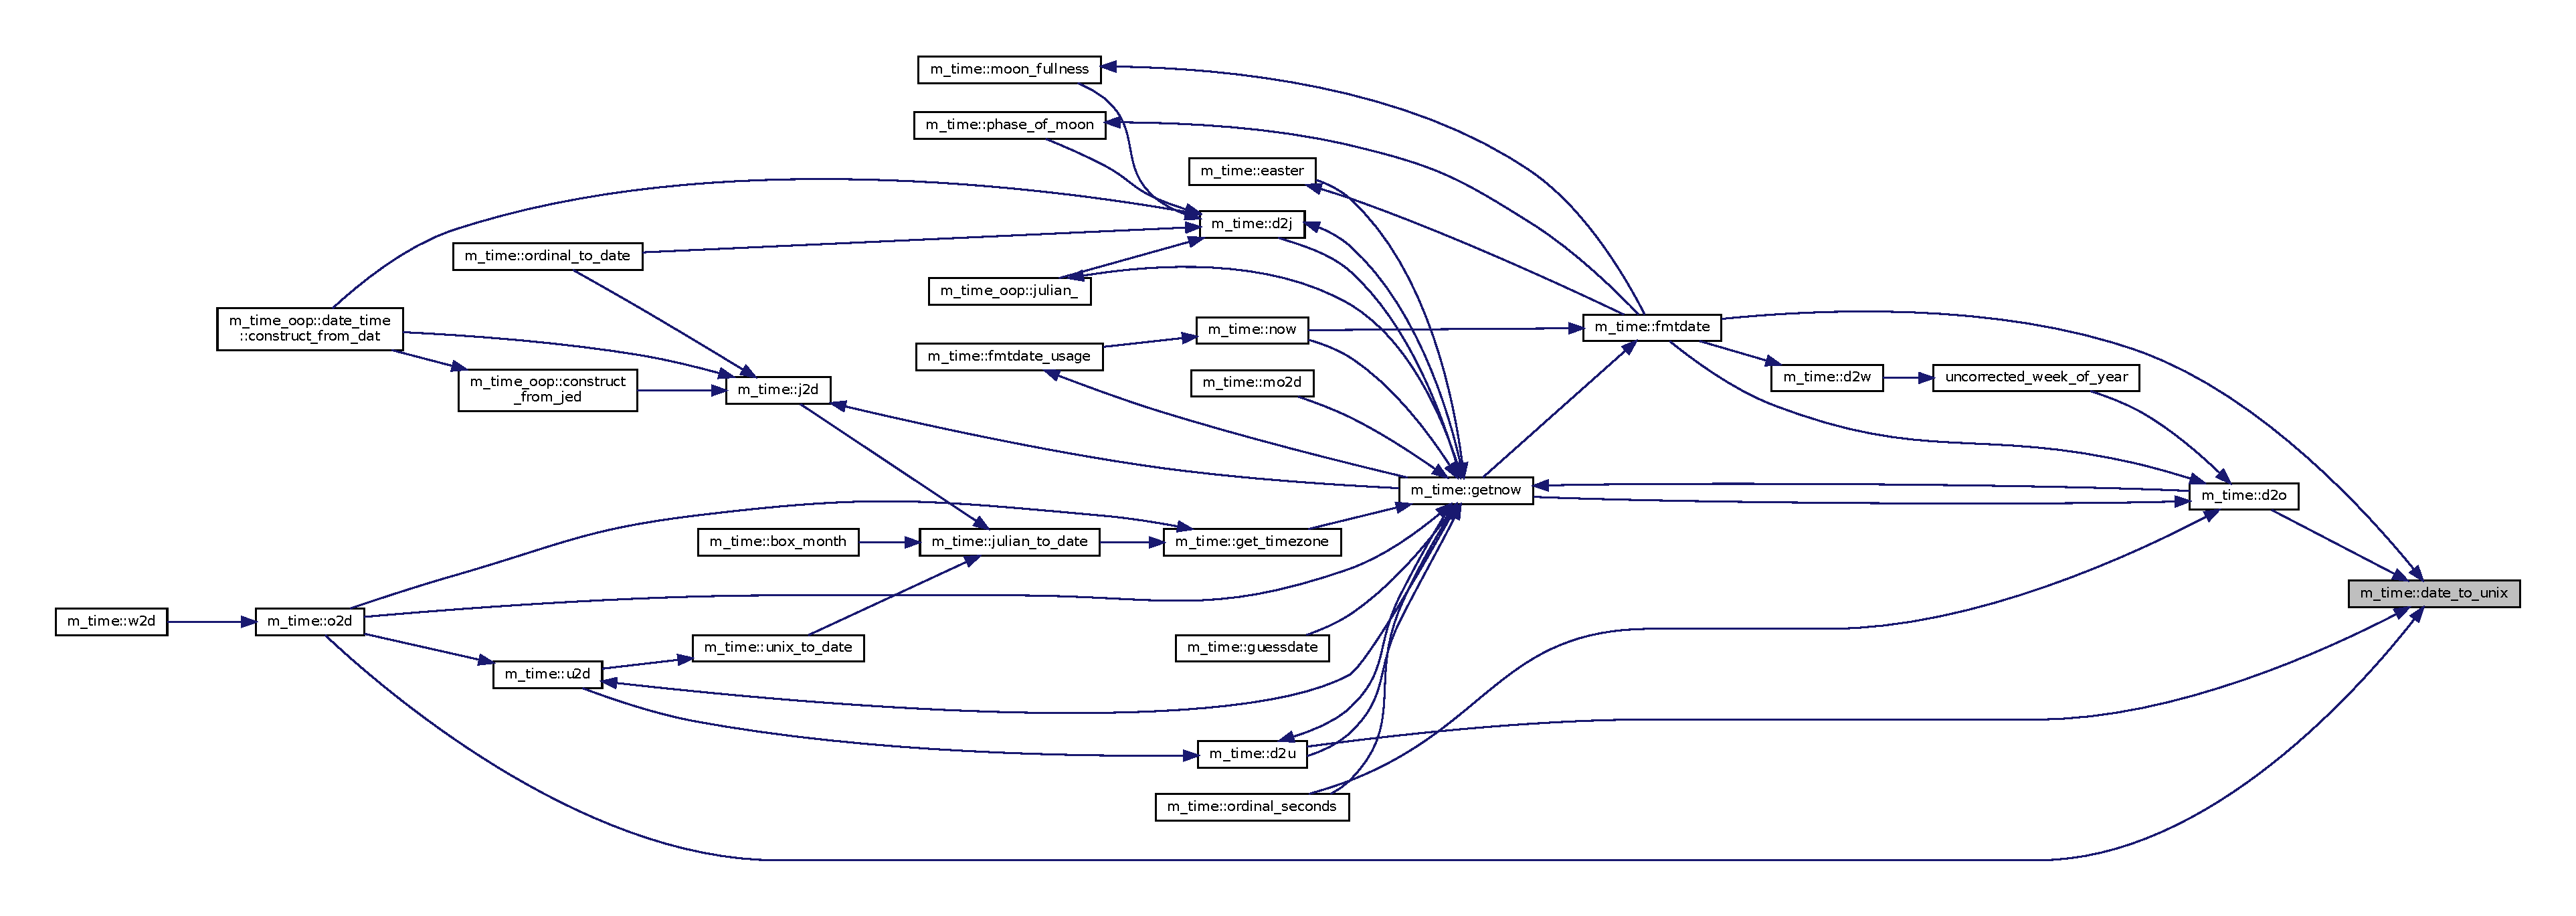
\includegraphics[width=350pt]{namespacem__time_aed245c691853279ebf0ce899dec9caa9_icgraph}
\end{center}
\end{figure}
\mbox{\Hypertarget{namespacem__time_a99393c7906f1989f90ece03969224938}\label{namespacem__time_a99393c7906f1989f90ece03969224938}} 
\index{m\_time@{m\_time}!days2sec@{days2sec}}
\index{days2sec@{days2sec}!m\_time@{m\_time}}
\doxysubsubsection{\texorpdfstring{days2sec()}{days2sec()}}
{\footnotesize\ttfamily real(kind=\mbox{\hyperlink{namespacem__time_ac10ea9e8d59ec74eaa7d89f2517d7422}{realtime}}) function, public m\+\_\+time\+::days2sec (\begin{DoxyParamCaption}\item[{character(len=$\ast$), intent(in)}]{str }\end{DoxyParamCaption})}

\hypertarget{namespacem__time_autotoc_md200}{}\doxysubsubsection{N\+A\+ME}\label{namespacem__time_autotoc_md200}
days2sec(3f) -\/ \mbox{[}M\+\_\+time\+:D\+U\+R\+A\+T\+I\+ON\mbox{]} convert string of form \mbox{[}\mbox{[}-\/\mbox{]}dd-\/\mbox{]}hh\+:mm\+:ss.\+nn to seconds (L\+I\+C\+E\+N\+SE\+:PD)\hypertarget{namespacem__time_autotoc_md201}{}\doxysubsubsection{S\+Y\+N\+O\+P\+S\+IS}\label{namespacem__time_autotoc_md201}
\begin{DoxyVerb}function days2sec(str) result(time)

 character(len=*),intent(in)       :: str
 real(kind=realtime)               :: time
\end{DoxyVerb}
\hypertarget{namespacem__time_autotoc_md202}{}\doxysubsubsection{D\+E\+S\+C\+R\+I\+P\+T\+I\+ON}\label{namespacem__time_autotoc_md202}
Given a string representing a duration of the form \char`\"{}\mbox{[}-\/\mbox{]}\mbox{[}\mbox{[}\mbox{[}dd-\/\mbox{]}hh\+:\mbox{]}mm\+:\mbox{]}ss\char`\"{} or \mbox{[}N\+Nd\mbox{]}\mbox{[}N\+Nh\mbox{]}\mbox{[}N\+Nm\mbox{[}\mbox{]}N\+Ns\mbox{]}\mbox{[}N\+Nw\mbox{]} return a value representing seconds.

If \char`\"{}dd-\/\char`\"{} is present, units for the numbers are assumed to proceed from day to hour to minute to second. But if no day is present, the units are assumed to proceed from second to minutes to hour from left to right. That is ... \begin{DoxyVerb}  [-]dd-hh:mm:ss
  [-]dd-hh:mm
  [-]dd-hh

  hh:mm:ss
  mm:ss
  ss

  Where dd is days, hh hours, mm minutes and ss seconds.
\end{DoxyVerb}


A decimal fraction is supported on the seconds (Actually, any of the numeric values may represent positive floating point numbers). Spaces are ignored.

Simple numeric values may also be used with unit suffixes; where s,m,h, or d represents seconds, minutes, hours or days and w represents a week. Allowed aliases for w,d,h,m, and s units are \begin{DoxyVerb} [NNd][NNh][NNm][NNs][NNw]

   d -  days,day
   m -  minutes,minute,min,mins
   h -  hours,hour,hr,hrs
   s -  seconds,second,sec,secs
   w -  week, weeks, wk, wks
\end{DoxyVerb}


The numeric values may represent floating point numbers.

Spaces, commas and case are ignored.\hypertarget{namespacem__time_autotoc_md203}{}\doxysubsubsection{O\+P\+T\+I\+O\+NS}\label{namespacem__time_autotoc_md203}
str string of the general form dd-\/hh\+:mm\+:ss.\+nn \hypertarget{namespacem__time_autotoc_md204}{}\doxysubsubsection{R\+E\+T\+U\+R\+NS}\label{namespacem__time_autotoc_md204}
time the number of seconds represented by the input string\hypertarget{namespacem__time_autotoc_md205}{}\doxysubsubsection{E\+X\+A\+M\+P\+LE}\label{namespacem__time_autotoc_md205}
\begin{DoxyVerb}Sample program:

 program demo_days2sec
 use M_time, only : days2sec
 implicit none
    write(*,*)days2sec('1-12:04:20')
    write(*,*)'one second ',days2sec('1')
    write(*,*)'one minute ',days2sec('1:00')
    write(*,*)'one hour ',days2sec('1:00:00')
    write(*,*)'one day ',days2sec('1-00:00:00')
    write(*,*)nint(days2sec(' 1-12:04:20              ')) .eq. 129860
    write(*,*)nint(days2sec(' 1.5 days                ')) .eq. 129600
    write(*,*)nint(days2sec(' 1.5 days 4hrs 30minutes ')) .eq. 145800
    write(*,*)nint(days2sec(' 1.5d                    ')) .eq. 129600
    write(*,*)nint(days2sec(' 1d2h3m4s                ')) .eq. 93784
    ! duplicates
    write(*,*)nint(days2sec(' 1d1d1d                  ')) .eq. 259200
    ! negative values
    write(*,*)nint(days2sec(' 4d-12h                  ')) .eq. 302400
 end program demo_days2sec

Results:

 > 129860.00000000000
 > one second    1.0000000000000000
 > one minute    60.000000000000000
 > one hour    3600.0000000000000
 > one day    86400.000000000000
 > T
 > T
 > T
 > T
 > T
 > T
 > T
\end{DoxyVerb}
\hypertarget{namespacem__time_autotoc_md206}{}\doxysubsubsection{A\+U\+T\+H\+OR}\label{namespacem__time_autotoc_md206}
John S. Urban, 2015 \hypertarget{namespacem__time_autotoc_md207}{}\doxysubsubsection{L\+I\+C\+E\+N\+SE}\label{namespacem__time_autotoc_md207}
Public Domain 

References m\+\_\+time\+\_\+duplicate\+::compact(), m\+\_\+time\+\_\+duplicate\+::lower(), m\+\_\+time\+\_\+duplicate\+::s2v(), m\+\_\+time\+\_\+duplicate\+::split(), m\+\_\+time\+\_\+duplicate\+::substitute(), and m\+\_\+time\+\_\+duplicate\+::transliterate().

Here is the call graph for this function\+:\nopagebreak
\begin{figure}[H]
\begin{center}
\leavevmode
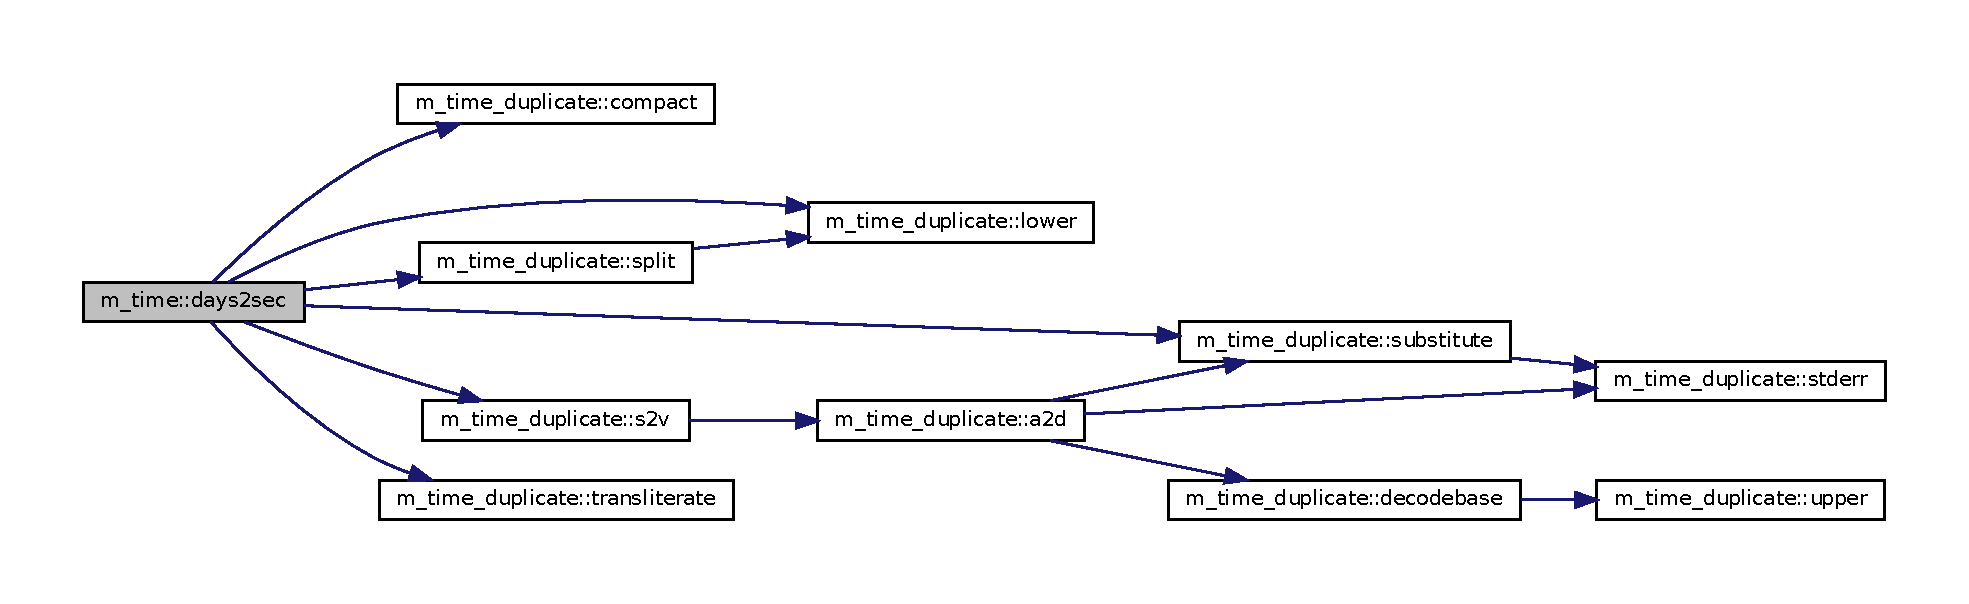
\includegraphics[width=350pt]{namespacem__time_a99393c7906f1989f90ece03969224938_cgraph}
\end{center}
\end{figure}
\mbox{\Hypertarget{namespacem__time_adfda8a89820b8d0ad4581a14896e4ce5}\label{namespacem__time_adfda8a89820b8d0ad4581a14896e4ce5}} 
\index{m\_time@{m\_time}!dow@{dow}}
\index{dow@{dow}!m\_time@{m\_time}}
\doxysubsubsection{\texorpdfstring{dow()}{dow()}}
{\footnotesize\ttfamily subroutine, public m\+\_\+time\+::dow (\begin{DoxyParamCaption}\item[{integer, dimension(8), intent(in)}]{values,  }\item[{integer, intent(out), optional}]{weekday,  }\item[{character(len=$\ast$), intent(out), optional}]{day,  }\item[{integer, intent(out), optional}]{ierr }\end{DoxyParamCaption})}

\hypertarget{namespacem__time_autotoc_md115}{}\doxysubsubsection{N\+A\+ME}\label{namespacem__time_autotoc_md115}
dow(3f) -\/ \mbox{[}M\+\_\+time\+:D\+A\+Y\+\_\+\+O\+F\+\_\+\+W\+E\+EK\mbox{]} given a date-\/time array D\+AT return the day of the week (L\+I\+C\+E\+N\+SE\+:PD)\hypertarget{namespacem__time_autotoc_md116}{}\doxysubsubsection{S\+Y\+N\+O\+P\+S\+IS}\label{namespacem__time_autotoc_md116}
\begin{DoxyVerb}subroutine dow(values, weekday, day, ierr)

 integer,intent(in) :: values(8)
 integer,intent(out),optional :: weekday
 character(len=*),intent(out),optional :: day
 integer,intent(out),optional :: ierr
\end{DoxyVerb}
\hypertarget{namespacem__time_autotoc_md117}{}\doxysubsubsection{D\+E\+S\+C\+R\+I\+P\+T\+I\+ON}\label{namespacem__time_autotoc_md117}
Given a date array D\+AT return the day of the week as a number and a name, Mon=1.\hypertarget{namespacem__time_autotoc_md118}{}\doxysubsubsection{O\+P\+T\+I\+O\+NS}\label{namespacem__time_autotoc_md118}
values \char`\"{}\+D\+A\+T\char`\"{} array (an integer array of the same format as the array returned by the intrinsic D\+A\+T\+E\+\_\+\+A\+N\+D\+\_\+\+T\+I\+M\+E(3f)) describing the date to be used to calculate the day of the week. \hypertarget{namespacem__time_autotoc_md119}{}\doxysubsubsection{R\+E\+T\+U\+R\+NS}\label{namespacem__time_autotoc_md119}
weekday The numeric day of the week, starting with Monday=1. Optional. day The name of the day of the week. Optional. ierr Error code \begin{DoxyVerb}     o [ 0] correct
     o [-1] invalid input date
     o [-2] neither day nor weekday
       return values were requested.

     If the error code is not returned and an error occurs,
     the program is stopped.
\end{DoxyVerb}
\hypertarget{namespacem__time_autotoc_md120}{}\doxysubsubsection{E\+X\+A\+M\+P\+LE}\label{namespacem__time_autotoc_md120}
\begin{DoxyVerb}Sample program:

 program demo_dow
 use M_time, only : dow
 implicit none
 integer          :: dat(8)     ! input date array
 integer          :: weekday
 character(len=9) :: day
 integer          :: ierr
   call date_and_time(values=dat)
   call dow(dat, weekday, day, ierr)
   write(*,'(a,i0)')'weekday=',weekday
   write(*,'(a,a)')'day=',trim(day)
   write(*,'(a,i0)')'ierr=',ierr
 end program demo_dow

results:

 weekday=1
 day=Monday
 ierr=0
\end{DoxyVerb}
 \hypertarget{namespacem__time_autotoc_md121}{}\doxysubsubsection{A\+U\+T\+H\+OR}\label{namespacem__time_autotoc_md121}
John S. Urban, 2015-\/12-\/19 \hypertarget{namespacem__time_autotoc_md122}{}\doxysubsubsection{L\+I\+C\+E\+N\+SE}\label{namespacem__time_autotoc_md122}
Public Domain 

References date\+\_\+to\+\_\+julian().

Here is the call graph for this function\+:\nopagebreak
\begin{figure}[H]
\begin{center}
\leavevmode
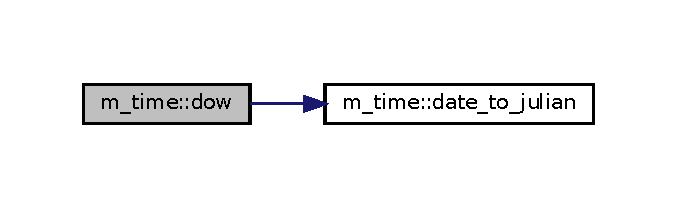
\includegraphics[width=325pt]{namespacem__time_adfda8a89820b8d0ad4581a14896e4ce5_cgraph}
\end{center}
\end{figure}
Here is the caller graph for this function\+:\nopagebreak
\begin{figure}[H]
\begin{center}
\leavevmode
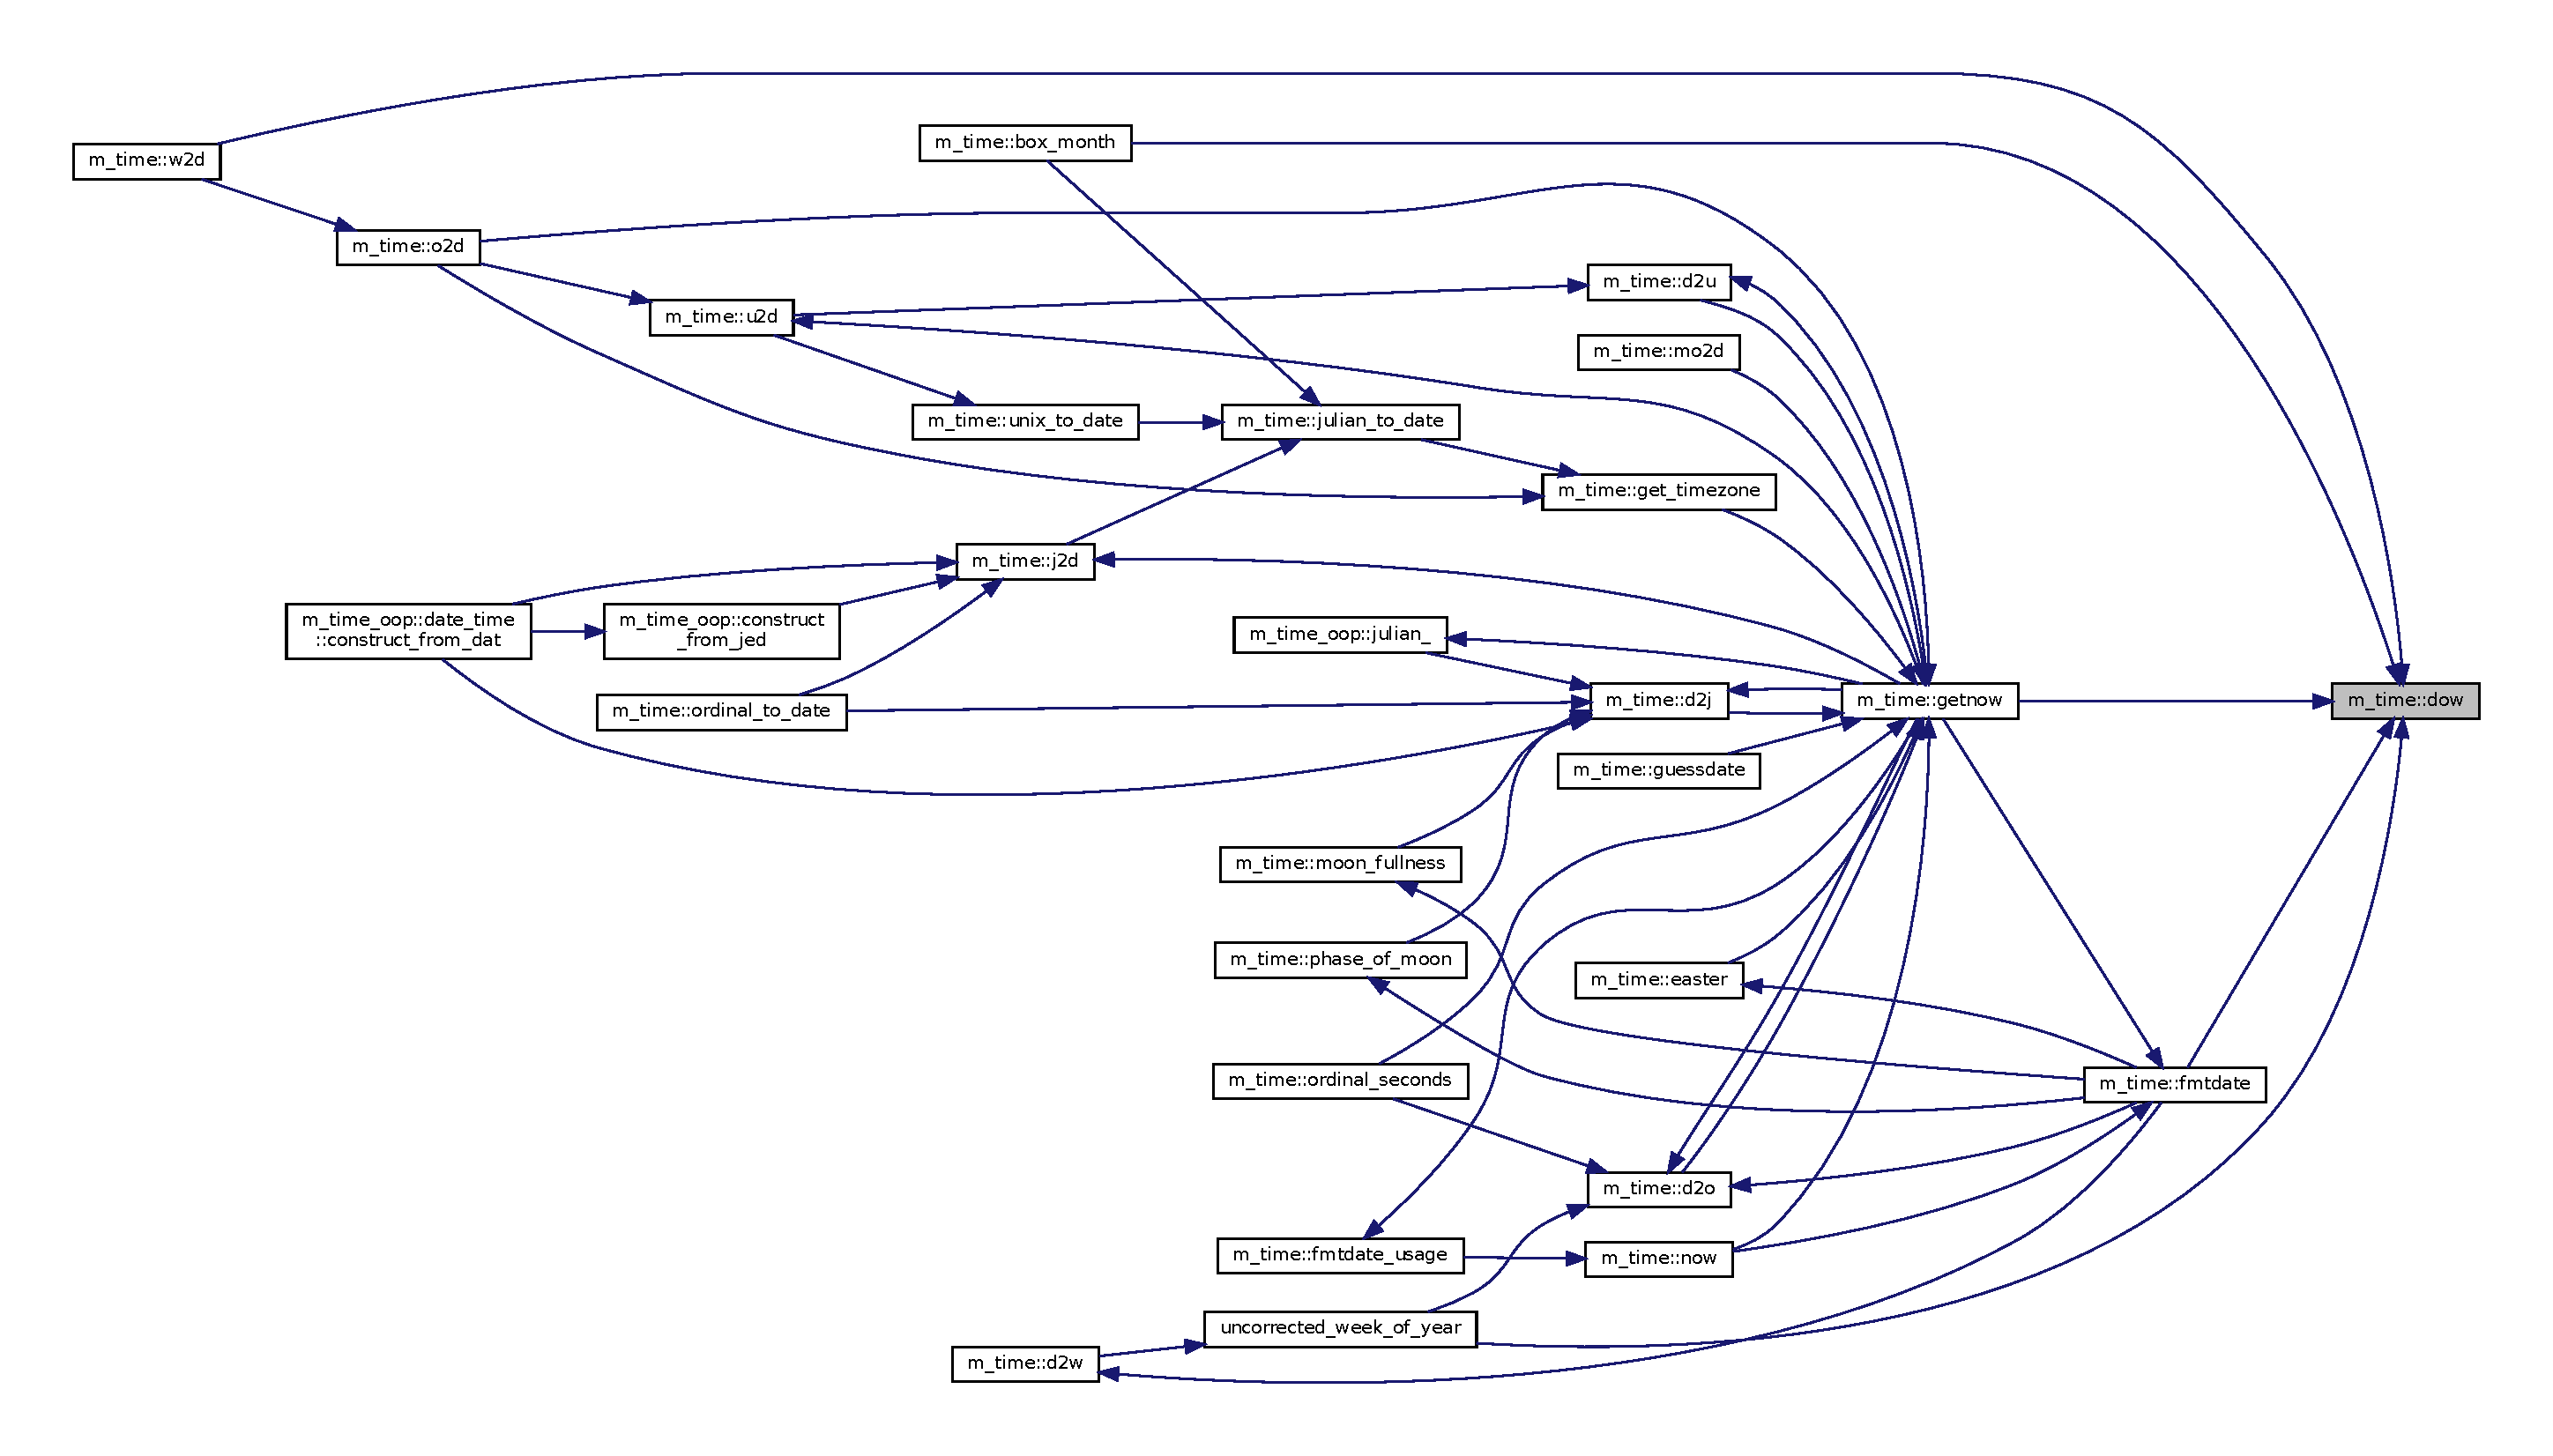
\includegraphics[width=350pt]{namespacem__time_adfda8a89820b8d0ad4581a14896e4ce5_icgraph}
\end{center}
\end{figure}
\mbox{\Hypertarget{namespacem__time_a5ccb70e20160fcf26bb403dbff1f138a}\label{namespacem__time_a5ccb70e20160fcf26bb403dbff1f138a}} 
\index{m\_time@{m\_time}!easter@{easter}}
\index{easter@{easter}!m\_time@{m\_time}}
\doxysubsubsection{\texorpdfstring{easter()}{easter()}}
{\footnotesize\ttfamily subroutine, public m\+\_\+time\+::easter (\begin{DoxyParamCaption}\item[{integer, intent(in)}]{year,  }\item[{integer, dimension(8), intent(out)}]{dat }\end{DoxyParamCaption})}

\hypertarget{namespacem__time_autotoc_md222}{}\doxysubsubsection{N\+A\+ME}\label{namespacem__time_autotoc_md222}
easter(3f) -\/ \mbox{[}M\+\_\+time\+:A\+S\+T\+R\+O\+L\+O\+G\+I\+C\+AL\mbox{]} calculate date for Easter given a year (L\+I\+C\+E\+N\+SE\+:PD)\hypertarget{namespacem__time_autotoc_md223}{}\doxysubsubsection{S\+Y\+N\+O\+P\+S\+IS}\label{namespacem__time_autotoc_md223}
subroutine easter(year,dat)

integer, intent(in) \+:: year integer, intent(out) \+:: dat\hypertarget{namespacem__time_autotoc_md224}{}\doxysubsubsection{D\+E\+S\+C\+R\+I\+P\+T\+I\+ON}\label{namespacem__time_autotoc_md224}
The Date of Easter (Sunday)

The algorithm is due to J.-\/M. Oudin (1940) and is reprinted in the Explanatory Supplement to the Astronomical Almanac, ed. P. K. Seidelmann (1992). See Chapter 12, \char`\"{}\+Calendars\char`\"{}, by L. E. Doggett.

The following are dates of Easter from 1980 to 2024\+: \begin{DoxyVerb} 1980  April  6        1995  April 16        2010  April  4
 1981  April 19        1996  April  7        2011  April 24
 1982  April 11        1997  March 30        2012  April  8
 1983  April  3        1998  April 12        2013  March 31
 1984  April 22        1999  April  4        2014  April 20
 1985  April  7        2000  April 23        2015  April  5
 1986  March 30        2001  April 15        2016  March 27
 1987  April 19        2002  March 31        2017  April 16
 1988  April  3        2003  April 20        2018  April  1
 1989  March 26        2004  April 11        2019  April 21
 1990  April 15        2005  March 27        2020  April 12
 1991  March 31        2006  April 16        2021  April  4
 1992  April 19        2007  April  8        2022  April 17
 1993  April 11        2008  March 23        2023  April  9
 1994  April  3        2009  April 12        2024  March 31
\end{DoxyVerb}


N.\+B. The date of Easter for the Eastern Orthodox Church may be different.\hypertarget{namespacem__time_autotoc_md225}{}\doxysubsubsection{O\+P\+T\+I\+O\+NS}\label{namespacem__time_autotoc_md225}
year Year for which to calculate day that Easter falls on \hypertarget{namespacem__time_autotoc_md226}{}\doxysubsubsection{R\+E\+S\+U\+L\+TS}\label{namespacem__time_autotoc_md226}
dat Date array for noon on Easter for the specified year\hypertarget{namespacem__time_autotoc_md227}{}\doxysubsubsection{E\+X\+A\+M\+P\+LE}\label{namespacem__time_autotoc_md227}
\begin{DoxyVerb}Sample program:

 program demo_easter
 use M_time, only : easter, fmtdate
 implicit none
 integer :: year
 integer :: dat(8) ! year,month,day,tz,hour,minute,second,millisecond
   call date_and_time(values=dat)  ! get current year
   year=dat(1)
   call easter(year, dat)
   write(*,*)fmtdate(dat,&
   "Easter day: the %d day of %L in the year of our Lord %Y")
 end program demo_easter

Sample output:

 Easter day: the 16th day of April in the year of our Lord 2017
\end{DoxyVerb}


U.\+S. Naval Observatory Astronomical Applications Department

This code assembled by Alan Miller Reference web site\+: \href{http://aa.usno.navy.mil/faq/docs/easter.html}{\texttt{ http\+://aa.\+usno.\+navy.\+mil/faq/docs/easter.\+html}} Latest revision 8 April 2002 Here is the caller graph for this function\+:\nopagebreak
\begin{figure}[H]
\begin{center}
\leavevmode
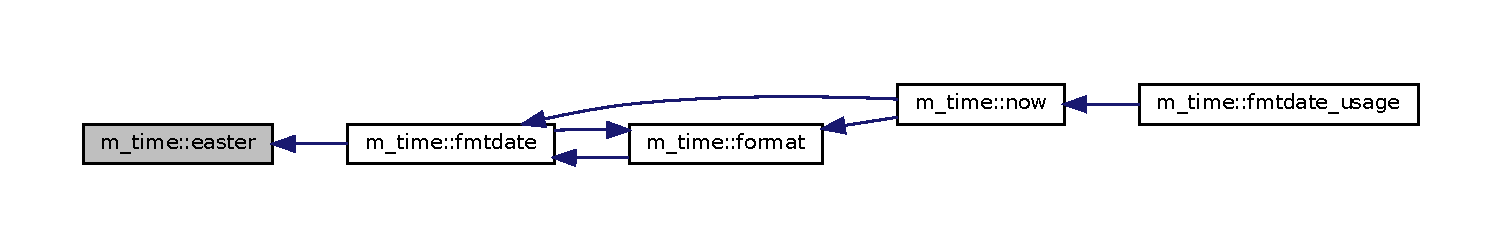
\includegraphics[width=350pt]{namespacem__time_a5ccb70e20160fcf26bb403dbff1f138a_icgraph}
\end{center}
\end{figure}
\mbox{\Hypertarget{namespacem__time_a2cb84c9b8af4f395b76aed76e1431328}\label{namespacem__time_a2cb84c9b8af4f395b76aed76e1431328}} 
\index{m\_time@{m\_time}!fmtdate@{fmtdate}}
\index{fmtdate@{fmtdate}!m\_time@{m\_time}}
\doxysubsubsection{\texorpdfstring{fmtdate()}{fmtdate()}}
{\footnotesize\ttfamily character(len=\+:) function, allocatable, public m\+\_\+time\+::fmtdate (\begin{DoxyParamCaption}\item[{integer, dimension(8), intent(in)}]{values,  }\item[{character(len=$\ast$), intent(in), optional}]{format }\end{DoxyParamCaption})}

\hypertarget{namespacem__time_autotoc_md94}{}\doxysubsubsection{N\+A\+ME}\label{namespacem__time_autotoc_md94}
fmtdate(3f) -\/ \mbox{[}M\+\_\+time\+:D\+A\+T\+E\+\_\+\+P\+R\+I\+N\+T\+I\+NG\mbox{]} given D\+AT date-\/time array return date as string using specified format (L\+I\+C\+E\+N\+SE\+:PD)\hypertarget{namespacem__time_autotoc_md95}{}\doxysubsubsection{S\+Y\+N\+O\+P\+S\+IS}\label{namespacem__time_autotoc_md95}
\begin{DoxyVerb}function fmtdate(values,format) RESULT (timestr)

 integer,dimension(8),intent(in)      :: values
 character(len=*),intent(in),optional :: format
 character(len=:),allocatable         :: timestr
\end{DoxyVerb}
\hypertarget{namespacem__time_autotoc_md96}{}\doxysubsubsection{D\+E\+S\+C\+R\+I\+P\+T\+I\+ON}\label{namespacem__time_autotoc_md96}
The fmtdate(3f) procedure lets you reformat a D\+AT array in many common formats using a special string containing macro names beginning with \textquotesingle{}\textquotesingle{}. To see the allowable macros call or see the fmtdate\+\_\+usage(3f) routine.\hypertarget{namespacem__time_autotoc_md97}{}\doxysubsubsection{O\+P\+T\+I\+O\+NS}\label{namespacem__time_autotoc_md97}
values date in a \char`\"{}\+D\+A\+T\char`\"{} array, which is the same format as the values returned by the intrinsic D\+A\+T\+E\+\_\+\+A\+N\+D\+\_\+\+T\+I\+M\+E(3f)\+:

dat=\mbox{[} year,month,day,timezone,hour,\& \& minutes,seconds,milliseconds\mbox{]}

format string describing how to format the \char`\"{}\+D\+A\+T\char`\"{} array. For a complete description of the formatting macros supported see fmtdate\+\_\+usage(3f). \hypertarget{namespacem__time_autotoc_md98}{}\doxysubsubsection{R\+E\+T\+U\+R\+NS}\label{namespacem__time_autotoc_md98}
timestr formatted output string representing date\hypertarget{namespacem__time_autotoc_md99}{}\doxysubsubsection{E\+X\+A\+M\+P\+LE}\label{namespacem__time_autotoc_md99}
\begin{DoxyVerb}Sample program:

 program demo_fmtdate
 use M_time, only : fmtdate
 implicit none
 integer :: dat(8)
    call date_and_time(values=dat)
    write(*,*)fmtdate(dat,"current date: %w, %l %d, %Y %H:%m:%s %N")
    call showme()
 contains
 subroutine showme()
    use M_time, only : fmtdate_usage
    call fmtdate_usage() ! see all formatting options
 end subroutine showme
 end program demo_fmtdate

results:

   The current date is Sun, Jul 17th, 2016 01:21:35 PM
    ::
    :: An up-to-date description of all the
    :: formatting options will appear here
    ::
\end{DoxyVerb}
\hypertarget{namespacem__time_autotoc_md100}{}\doxysubsubsection{A\+U\+T\+H\+OR}\label{namespacem__time_autotoc_md100}
John S. Urban, 2015-\/12-\/19 \hypertarget{namespacem__time_autotoc_md101}{}\doxysubsubsection{L\+I\+C\+E\+N\+SE}\label{namespacem__time_autotoc_md101}
Public Domain 

References d2o(), d2w(), date\+\_\+to\+\_\+julian(), date\+\_\+to\+\_\+unix(), dow(), easter(), moon\+\_\+fullness(), phase\+\_\+of\+\_\+moon(), m\+\_\+time\+\_\+duplicate\+::substitute(), and v2mo().

Here is the call graph for this function\+:\nopagebreak
\begin{figure}[H]
\begin{center}
\leavevmode
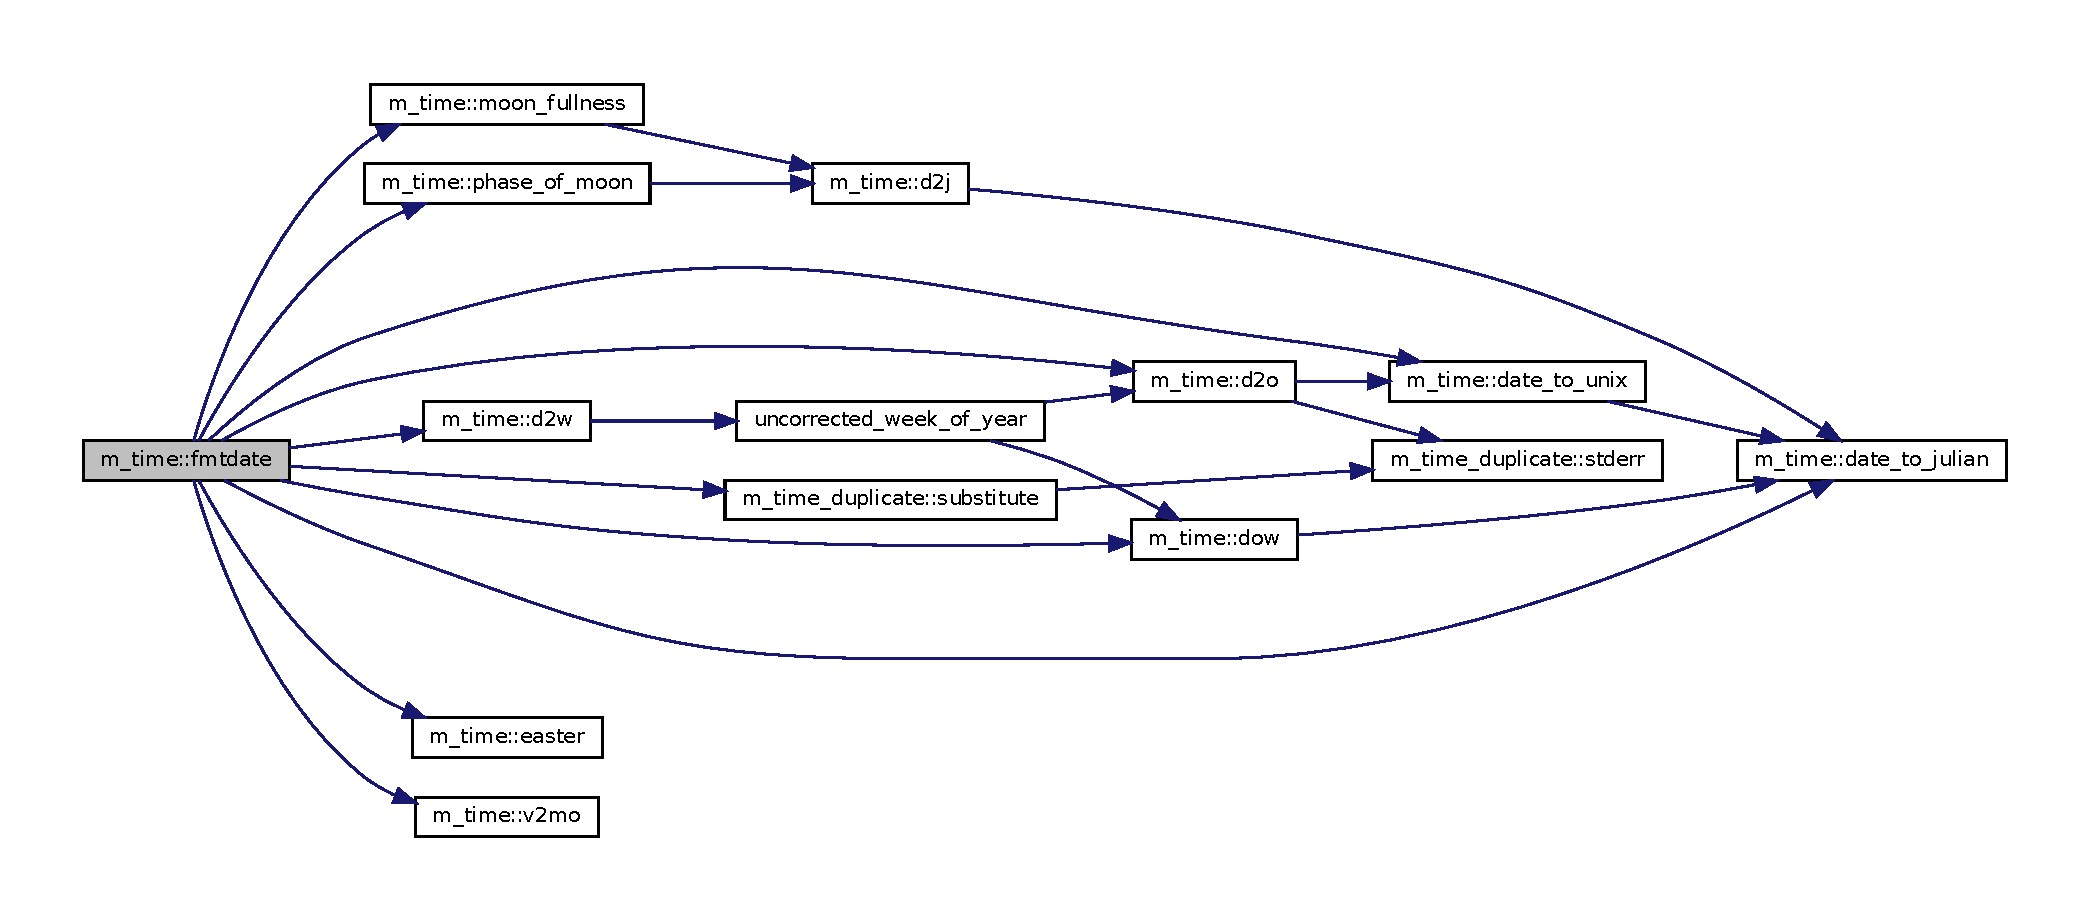
\includegraphics[width=350pt]{namespacem__time_a2cb84c9b8af4f395b76aed76e1431328_cgraph}
\end{center}
\end{figure}
Here is the caller graph for this function\+:\nopagebreak
\begin{figure}[H]
\begin{center}
\leavevmode
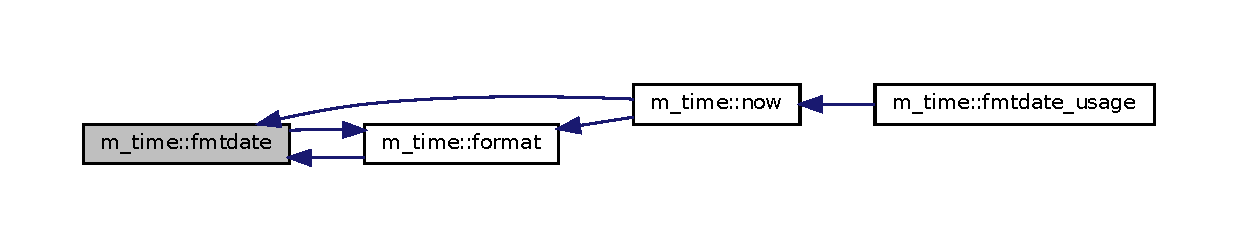
\includegraphics[width=350pt]{namespacem__time_a2cb84c9b8af4f395b76aed76e1431328_icgraph}
\end{center}
\end{figure}
\mbox{\Hypertarget{namespacem__time_a914927f70fb9495af1be2e484b967111}\label{namespacem__time_a914927f70fb9495af1be2e484b967111}} 
\index{m\_time@{m\_time}!fmtdate\_usage@{fmtdate\_usage}}
\index{fmtdate\_usage@{fmtdate\_usage}!m\_time@{m\_time}}
\doxysubsubsection{\texorpdfstring{fmtdate\_usage()}{fmtdate\_usage()}}
{\footnotesize\ttfamily subroutine, public m\+\_\+time\+::fmtdate\+\_\+usage (\begin{DoxyParamCaption}\item[{integer, intent(in), optional}]{indent }\end{DoxyParamCaption})}

\hypertarget{namespacem__time_autotoc_md102}{}\doxysubsubsection{N\+A\+ME}\label{namespacem__time_autotoc_md102}
fmtdate\+\_\+usage(3f) -\/ \mbox{[}M\+\_\+time\+:D\+A\+T\+E\+\_\+\+P\+R\+I\+N\+T\+I\+NG\mbox{]} display macros recognized by fmtdate(3f) and now(3f) (L\+I\+C\+E\+N\+SE\+:PD)\hypertarget{namespacem__time_autotoc_md103}{}\doxysubsubsection{S\+Y\+N\+O\+P\+S\+IS}\label{namespacem__time_autotoc_md103}
\begin{DoxyVerb}subroutine fmtdate_usage(indent)

 integer,intent(in),optional      :: indent
\end{DoxyVerb}
\hypertarget{namespacem__time_autotoc_md104}{}\doxysubsubsection{D\+E\+S\+C\+R\+I\+P\+T\+I\+ON}\label{namespacem__time_autotoc_md104}
The fmtdate\+\_\+usage(3f) subroutine displays the formatting options available for use in procedures such as fmtdate(3f) and now(3f). It is typically used to produce up-\/to-\/date help text in commands that use the M\+\_\+time(3fm) module, so that the formatting information only needs maintained in one place (this routine) and is easily displayed so users can quickly obtain a description of the formatting macros.\hypertarget{namespacem__time_autotoc_md105}{}\doxysubsubsection{O\+P\+T\+I\+O\+NS}\label{namespacem__time_autotoc_md105}
indent how many spaces to prefix the output with, so that calling programs can position the output. Default for this optional parameter is three (3).\hypertarget{namespacem__time_autotoc_md106}{}\doxysubsubsection{E\+X\+A\+M\+P\+LE}\label{namespacem__time_autotoc_md106}
\begin{DoxyVerb}Sample Program:

 program demo_fmtdate_usage
 use M_time, only : fmtdate_usage
 implicit none
    call fmtdate_usage() ! see all formatting options
 end program demo_fmtdate_usage

results (actually call the routine to ensure this is up to date):

 Description                                        Example

 Base time array:
 (1) %Y -- year, yyyy                                2016
 (2) %M -- month of year, 01 to 12                   07
 (3) %D -- day of month, 01 to 31                    29
     %d -- day of month, with suffix (1st, 2nd,...)  29th
 (4) %Z -- minutes from UTC                          -0240
     %z -- -+hh:mm from UTC                          -04:00
     %T -- -+hhmm  from UTC                          -0400
 (5) %h -- hours, 00 to 23                           10
     %H -- hour (1 to 12, or twelve-hour clock)      10
     %N -- midnight< AM <=noon; noon<= PM <midnight  AM
 (6) %m -- minutes, 00 to 59                         54
 (7) %s -- sec, 00 to 59                             08
 (8) %x -- milliseconds 000 to 999                   521
 Conversions:
     %E -- Unix Epoch time                           1469804048.5220029
     %e -- integer value of Unix Epoch time          1469804049
     %J -- Julian  date                              2457599.121
     %j -- integer value of Julian Date(Julian Day)  2457599
     %O -- Ordinal day (day of year)                 211
     %o -- Whole days since Unix Epoch date          17011
     %U -- day of week, 1..7 Sunday=1                6
     %u -- day of week, 1..7 Monday=1                5
     %i -- ISO week of year 1..53                    30
     %I -- iso-8601 week-numbering date(yyyy-Www-d)  2016-W30-5
  Names:
     %l -- abbreviated month name                    Jul
     %L -- full month name                           July
     %w -- first three characters of weekday         Fri
     %W -- weekday name                              Friday
     %p -- phase of moon                             New
     %P -- percent of way from new to full moon      -1%
  Literals:
     %% -- a literal %                               %
     %t -- tab character
     %b -- blank character
     %B -- exclamation(bang) character
     %n -- new line (system dependent)
     %q -- single quote (apostrophe)
     %Q -- double quote
  Program timing:
     %c -- CPU_TIME(3f) output                     .21875000000000000
     %C -- number of times this routine is used    1
     %S -- seconds since last use of this format   .0000000000000000
     %k -- time in seconds from SYSTEM_CLOCK(3f)   723258.812
     %K -- time in clicks from SYSTEM_CLOCK(3f)    723258812

If no percent (%) is found in the format one of several
alternate substitutions occurs.

If the format is composed entirely of one of the following
keywords the following substitutions occur:

  "iso-8601",
  "iso"        ==> %Y-%M-%DT%h:%m:%s%z
  "iso-8601W",
  "isoweek"    ==> %I 2016-W30-5
  "sql"        ==> "%Y-%M-%D %h:%m:%s.%x"
  "sqlday"     ==> "%Y-%M-%D"
  "sqltime"    ==> "%h:%m:%s.%x"
  "rfc-2822"   ==> %w, %D %l %Y %h:%m:%s %T
  "rfc-3339"   ==> %Y-%M-%DT%h:%m:%s%z
  "date"       ==> %w %l %D %h:%m:%s UTC%z %Y
  "short"      ==> %w, %l %d, %Y %H:%m:%s %N UTC%z
  "long"," "   ==> %W, %L %d, %Y %H:%m:%s %N UTC%z
  "suffix"     ==> %Y%D%M%h%m%s
  "formal"     ==> The %d of %L %Y
  "lord"       ==> the %d day of %L in the year of our Lord %Y
  "easter"     ==> FOR THE YEAR OF THE CURRENT DATE:
                   Easter day: the %d day of %L in the year of our Lord %Y
  "all"        ==> A SAMPLE OF DATE FORMATS

otherwise the following words are replaced with the most
common macros:

numeric values:

   year     %Y  2016
   month    %M  07
   day      %D  29
   hour     %h  10
   minute   %m  54
   second   %s  08
   timezone %T  0400

   epoch    %e  1469804049
   julian   %j  2457599
   ordinal  %O  211
   weekday  %u  5

string values:

   MONTH    %L  July
   Month    %l  Jul
   WEEKDAY  %W  Thursday
   Weekday  %w  Thu
   DAY      %d  7th
   TIMEZONE %z  -04:00
   Timezone %Z  -240
   GOOD     %N  AM
   HOUR     %H  10

if none of these keywords are found then every letter that
is a macro is assumed to have an implied percent in front
of it. For example:

   YMDhms ==> %Y%M%D%h%m%s ==> 20160729105408
\end{DoxyVerb}
 \hypertarget{namespacem__time_autotoc_md107}{}\doxysubsubsection{A\+U\+T\+H\+OR}\label{namespacem__time_autotoc_md107}
John S. Urban, 2015-\/10-\/24 \hypertarget{namespacem__time_autotoc_md108}{}\doxysubsubsection{L\+I\+C\+E\+N\+SE}\label{namespacem__time_autotoc_md108}
Public Domain 

References now().

Here is the call graph for this function\+:\nopagebreak
\begin{figure}[H]
\begin{center}
\leavevmode
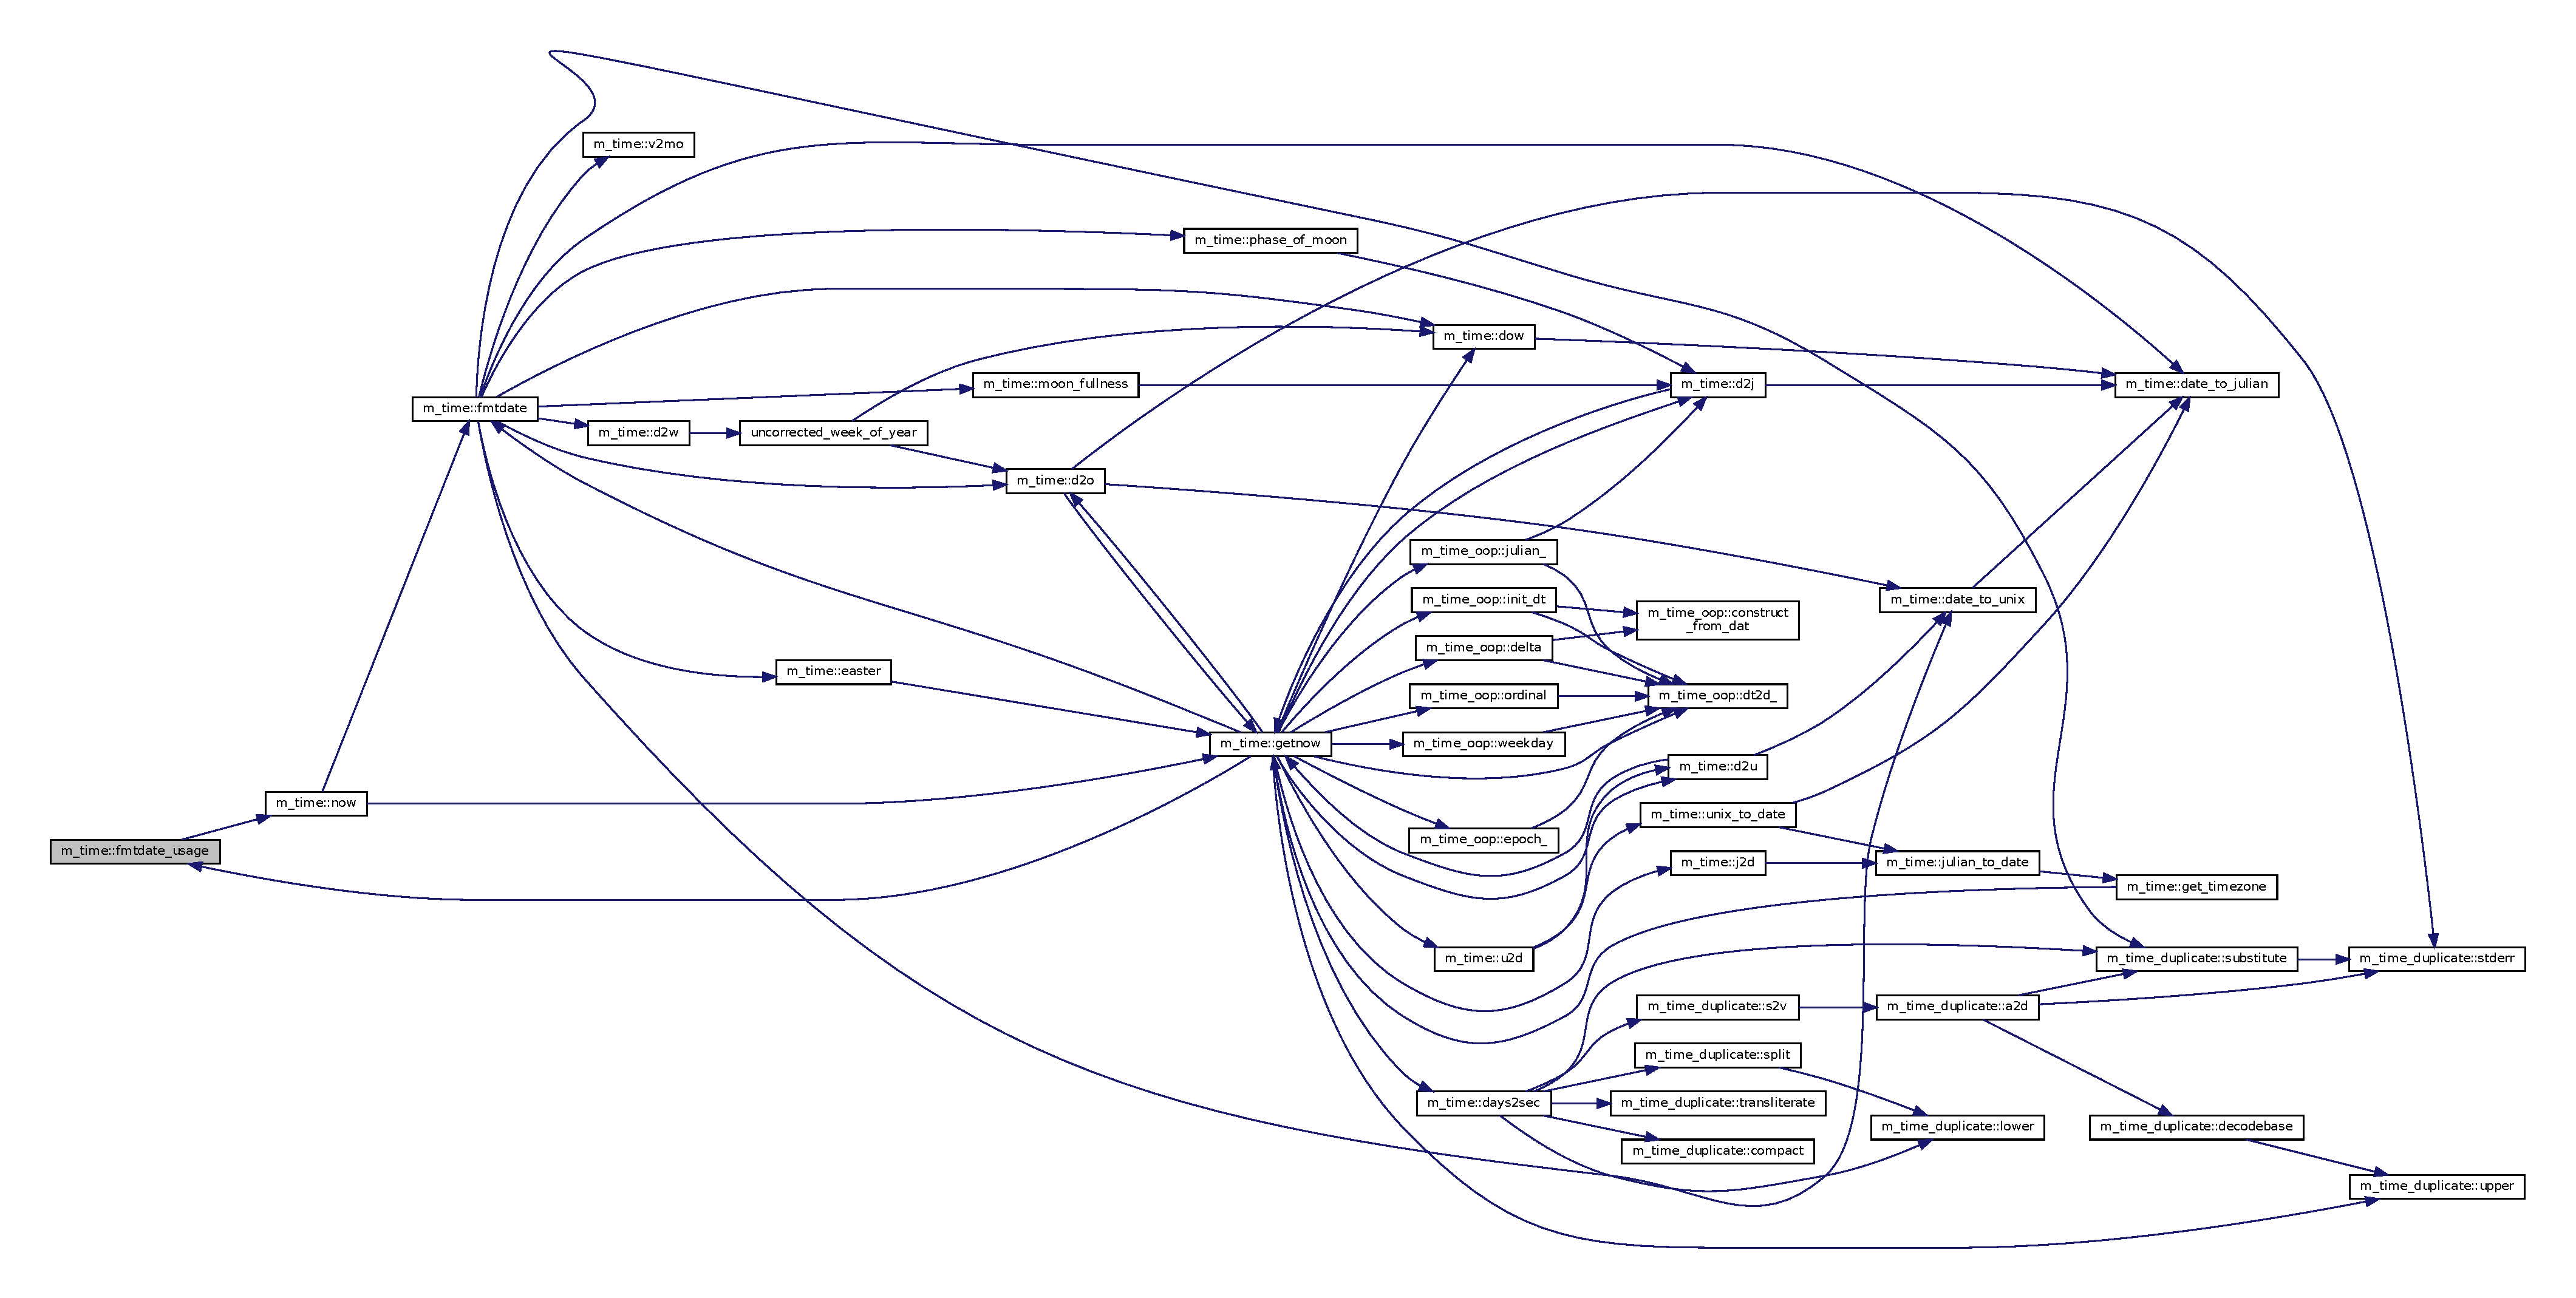
\includegraphics[width=350pt]{namespacem__time_a914927f70fb9495af1be2e484b967111_cgraph}
\end{center}
\end{figure}
\mbox{\Hypertarget{namespacem__time_a7903410a1d28bcdf3d33ab0c2d74b124}\label{namespacem__time_a7903410a1d28bcdf3d33ab0c2d74b124}} 
\index{m\_time@{m\_time}!get\_timezone@{get\_timezone}}
\index{get\_timezone@{get\_timezone}!m\_time@{m\_time}}
\doxysubsubsection{\texorpdfstring{get\_timezone()}{get\_timezone()}}
{\footnotesize\ttfamily integer function m\+\_\+time\+::get\+\_\+timezone\hspace{0.3cm}{\ttfamily [private]}}

Here is the caller graph for this function\+:\nopagebreak
\begin{figure}[H]
\begin{center}
\leavevmode
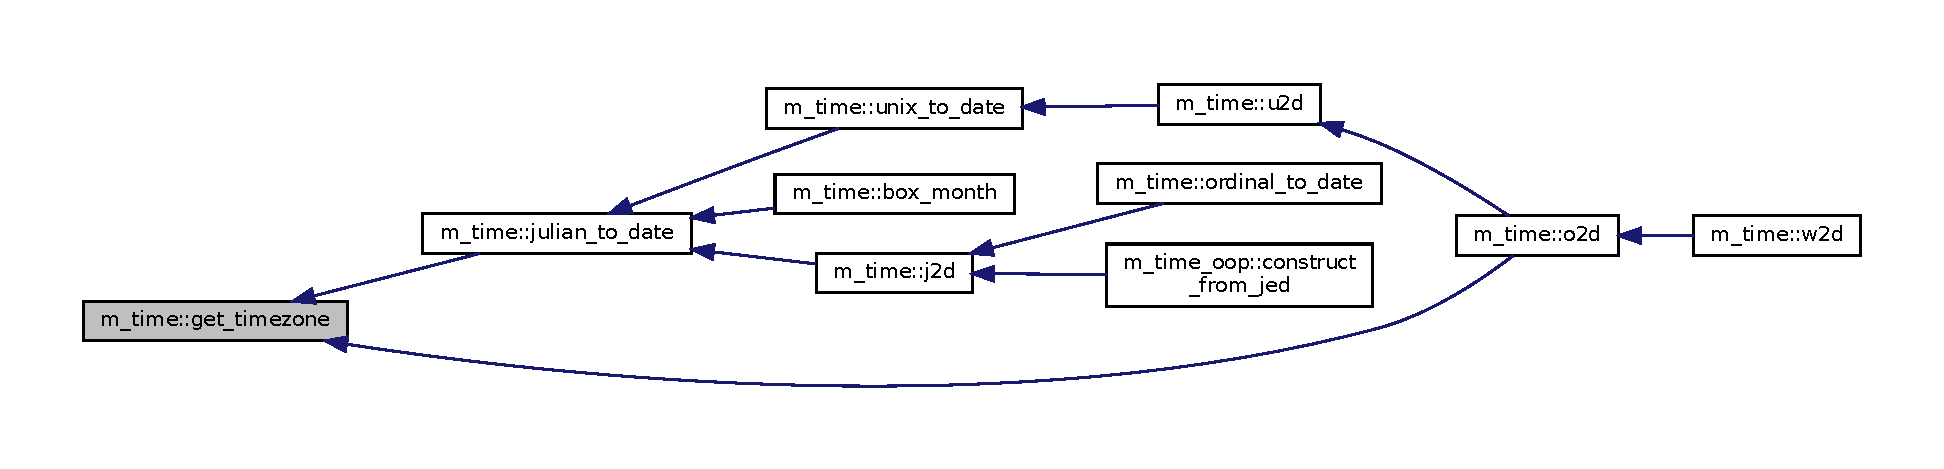
\includegraphics[width=350pt]{namespacem__time_a7903410a1d28bcdf3d33ab0c2d74b124_icgraph}
\end{center}
\end{figure}
\mbox{\Hypertarget{namespacem__time_aa5198c7aa4f3d8411c8ce93046ce3794}\label{namespacem__time_aa5198c7aa4f3d8411c8ce93046ce3794}} 
\index{m\_time@{m\_time}!guessdate@{guessdate}}
\index{guessdate@{guessdate}!m\_time@{m\_time}}
\doxysubsubsection{\texorpdfstring{guessdate()}{guessdate()}}
{\footnotesize\ttfamily subroutine, public m\+\_\+time\+::guessdate (\begin{DoxyParamCaption}\item[{character(len=$\ast$), intent(in)}]{datestring,  }\item[{integer, dimension(8), intent(out)}]{dat,  }\item[{integer, optional}]{ier }\end{DoxyParamCaption})}

\hypertarget{namespacem__time_autotoc_md109}{}\doxysubsubsection{N\+A\+ME}\label{namespacem__time_autotoc_md109}
guessdate(3f) -\/ \mbox{[}M\+\_\+time\+:R\+E\+A\+D\+I\+N\+G\+\_\+\+D\+A\+T\+ES\mbox{]} reads in a date, in various formats (L\+I\+C\+E\+N\+SE\+:PD)\hypertarget{namespacem__time_autotoc_md110}{}\doxysubsubsection{S\+Y\+N\+O\+P\+S\+IS}\label{namespacem__time_autotoc_md110}
\begin{DoxyVerb}subroutine guessdate(anot,dat)

 character(len=*),intent(in) :: anot
 integer,intent(out)         :: dat(8)
\end{DoxyVerb}
\hypertarget{namespacem__time_autotoc_md111}{}\doxysubsubsection{D\+E\+S\+C\+R\+I\+P\+T\+I\+ON}\label{namespacem__time_autotoc_md111}
Read in strings and except for looking for month names remove non-\/numeric characters and try to convert a string assumed to represent a date to a date-\/time array.

Years should always be expressed as four-\/digit numbers, and except for the special format yyyy-\/mm-\/dd the day should come after the year. Named months are preferred. If ambiguous the order is assumed to be day -\/ month -\/ year. Times are assumed to be of the form H\+H\+:\+MM\+:SS

It is planned that this routine will be superseded. As an alternative, a C routine exists in the standard C libraries that allows for expansive features when reading dates that can be called via the I\+S\+O\+\_\+\+C\+\_\+\+B\+I\+N\+D\+I\+NG interface.\hypertarget{namespacem__time_autotoc_md112}{}\doxysubsubsection{O\+P\+T\+I\+O\+NS}\label{namespacem__time_autotoc_md112}
anot A string assumed to represent a date including a year, month and day.

dat Integer array holding a \char`\"{}\+D\+A\+T\char`\"{} array, similar in structure to the array returned by the intrinsic D\+A\+T\+E\+\_\+\+A\+N\+D\+\_\+\+T\+I\+M\+E(3f)\+: \begin{DoxyVerb}   dat=[ year,month,day,timezone,hour,&
    & minutes,seconds,milliseconds]
\end{DoxyVerb}
\hypertarget{namespacem__time_autotoc_md113}{}\doxysubsubsection{E\+X\+A\+M\+P\+LE}\label{namespacem__time_autotoc_md113}
\begin{DoxyVerb}Sample program:

 program demo_guessdate
 use M_time, only : guessdate, fmtdate
 implicit none
 character(len=20),allocatable :: datestrings(:)
 character(len=:),allocatable  :: answer
 integer                       :: dat(8)
 integer                       :: i
    datestrings=[ &
    & 'January 9th, 2001   ',&
    & ' Tue Jul 19 2016    ',&
    & ' 21/12/2016         ',&
    & ' 4th of Jul 2004    ' ]
    do i=1,size(datestrings)
       write(*,'(a)')repeat('-',80)
       write(*,*)'TRYING ',datestrings(i)
       call guessdate(datestrings(i),dat)
       write(*,*)'DAT ARRAY ',dat
       answer=fmtdate(dat)
       write(*,*)'FOR '//datestrings(i)//' GOT '//trim(answer)
    enddo
 end program demo_guessdate

results:

 ---------------------------------------------------------------------
 TRYING January 9th, 2001
 DAT ARRAY         2001  1  9   -240    0   0   0    0
 FOR January 9th, 2001  GOT Tuesday, January 9th, 2001 12:00:00 AM
 ---------------------------------------------------------------------
 TRYING  Tue Jul 19 2016
 DAT ARRAY         2016  7  19  -240    0   0   0    0
 FOR  Tue Jul 19 2016   GOT Tuesday, July 19th, 2016 12:00:00 AM
 ---------------------------------------------------------------------
 TRYING  21/12/2016
 DAT ARRAY         2016  12 21  -240    0   0   0    0
 FOR  21/12/2016        GOT Wednesday, December 21st, 2016 12:00:00 AM
 ---------------------------------------------------------------------
 TRYING  4th of Jul 2004
 DAT ARRAY         2004  7  4   -240    0   0   0    0
 FOR  4th of Jul 2004   GOT Sunday, July 4th, 2004 12:00:00 AM
\end{DoxyVerb}
\hypertarget{namespacem__time_autotoc_md114}{}\doxysubsubsection{L\+I\+C\+E\+N\+SE}\label{namespacem__time_autotoc_md114}
Public Domain 

References m\+\_\+time\+\_\+duplicate\+::s2v(), m\+\_\+time\+\_\+duplicate\+::split(), m\+\_\+time\+\_\+duplicate\+::string\+\_\+to\+\_\+values(), m\+\_\+time\+\_\+duplicate\+::substitute(), and m\+\_\+time\+\_\+duplicate\+::upper().

Here is the call graph for this function\+:\nopagebreak
\begin{figure}[H]
\begin{center}
\leavevmode
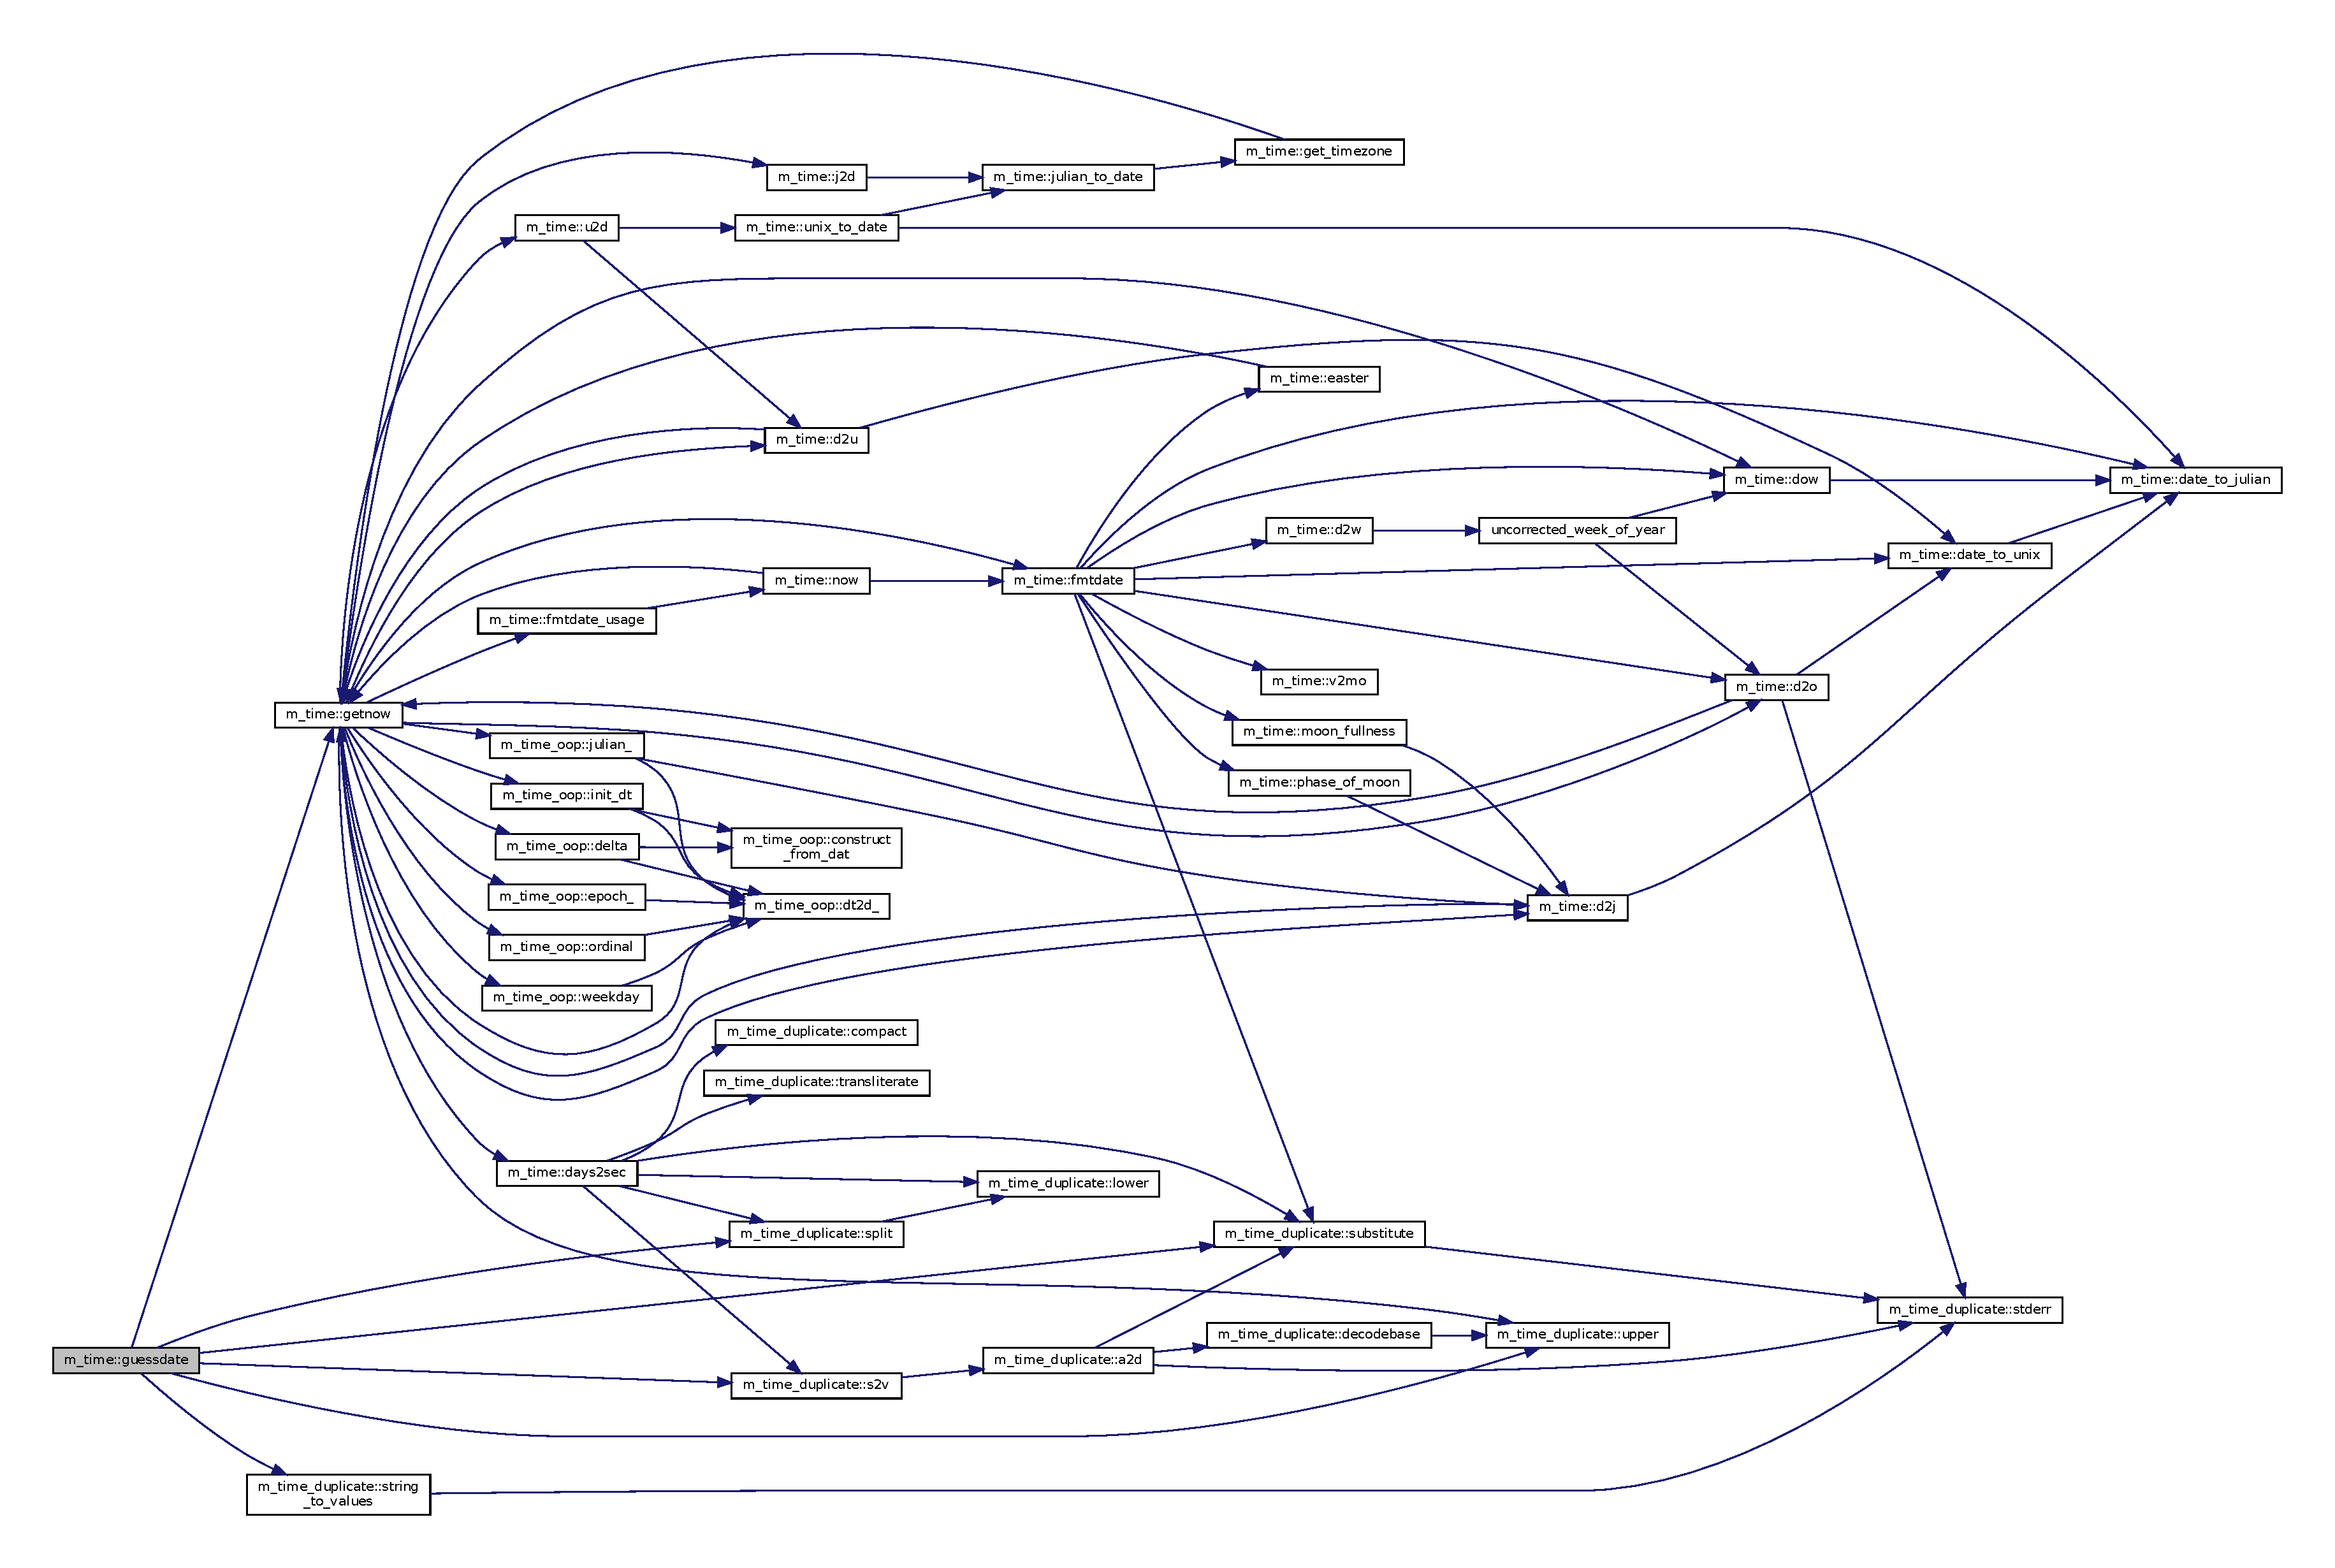
\includegraphics[width=350pt]{namespacem__time_aa5198c7aa4f3d8411c8ce93046ce3794_cgraph}
\end{center}
\end{figure}
\mbox{\Hypertarget{namespacem__time_a3ad5cad6df02c53e0429c3602a072e3c}\label{namespacem__time_a3ad5cad6df02c53e0429c3602a072e3c}} 
\index{m\_time@{m\_time}!j2d@{j2d}}
\index{j2d@{j2d}!m\_time@{m\_time}}
\doxysubsubsection{\texorpdfstring{j2d()}{j2d()}}
{\footnotesize\ttfamily integer function, dimension(8), public m\+\_\+time\+::j2d (\begin{DoxyParamCaption}\item[{real(kind=\mbox{\hyperlink{namespacem__time_ac10ea9e8d59ec74eaa7d89f2517d7422}{realtime}}), intent(in)}]{julian }\end{DoxyParamCaption})}

\hypertarget{namespacem__time_autotoc_md168}{}\doxysubsubsection{N\+A\+ME}\label{namespacem__time_autotoc_md168}
j2d(3f) -\/ \mbox{[}M\+\_\+time\+:J\+U\+L\+I\+AN\mbox{]} given a J\+ED (Julian Ephemeris Date) returns a date-\/time array D\+AT. (L\+I\+C\+E\+N\+SE\+:PD)\hypertarget{namespacem__time_autotoc_md169}{}\doxysubsubsection{S\+Y\+N\+O\+P\+S\+IS}\label{namespacem__time_autotoc_md169}
\begin{DoxyVerb}function j2d(julian) result (dat)

 real(kind=realtime),intent(in),optional :: julian
 integer                                 :: dat(8)
\end{DoxyVerb}
\hypertarget{namespacem__time_autotoc_md170}{}\doxysubsubsection{D\+E\+S\+C\+R\+I\+P\+T\+I\+ON}\label{namespacem__time_autotoc_md170}
Converts a Julian Ephemeris Date to a D\+AT date-\/time array.\hypertarget{namespacem__time_autotoc_md171}{}\doxysubsubsection{O\+P\+T\+I\+O\+NS}\label{namespacem__time_autotoc_md171}
julian A Julian Ephemeris Date (J\+ED) is the number of days since noon (not midnight) on January 1st, 4713 BC. If not present, use current time.\hypertarget{namespacem__time_autotoc_md172}{}\doxysubsubsection{R\+E\+T\+U\+R\+NS}\label{namespacem__time_autotoc_md172}
dat Integer array holding a \char`\"{}\+D\+A\+T\char`\"{} array, similar in structure to the array returned by the intrinsic D\+A\+T\+E\+\_\+\+A\+N\+D\+\_\+\+T\+I\+M\+E(3f)\+: \begin{DoxyVerb}   dat=[ year,month,day,timezone,hour,&
    & minutes,seconds,milliseconds]
\end{DoxyVerb}
\hypertarget{namespacem__time_autotoc_md173}{}\doxysubsubsection{E\+X\+A\+M\+P\+LE}\label{namespacem__time_autotoc_md173}
\begin{DoxyVerb}Sample program:

 program demo_j2d
 use M_time, only : j2d, d2j, fmtdate, realtime
 implicit none
 real(kind=realtime) :: today
 integer :: dat(8)
    call date_and_time(values=dat) ! get the date using intrinsic
    today=d2j(dat)                  ! convert today to Julian Date
    write(*,*)'Today=',fmtdate(j2d(today))
    ! math is easy with Julian Days and Julian Dates
    write(*,*)'Yesterday=',fmtdate(j2d(today-1.0d0))
    write(*,*)'Tomorrow=',fmtdate(j2d(today+1.0d0))
 end program demo_j2d

results:

 Today=Tuesday, July 19th, 2016 08:48:20 AM
 Yesterday=Monday, July 18th, 2016 08:48:20 AM
 Tomorrow=Wednesday, July 20th, 2016 08:48:20 AM
\end{DoxyVerb}
 \hypertarget{namespacem__time_autotoc_md174}{}\doxysubsubsection{A\+U\+T\+H\+OR}\label{namespacem__time_autotoc_md174}
John S. Urban, 2015 \hypertarget{namespacem__time_autotoc_md175}{}\doxysubsubsection{L\+I\+C\+E\+N\+SE}\label{namespacem__time_autotoc_md175}
Public Domain 

References julian\+\_\+to\+\_\+date().

Here is the call graph for this function\+:\nopagebreak
\begin{figure}[H]
\begin{center}
\leavevmode
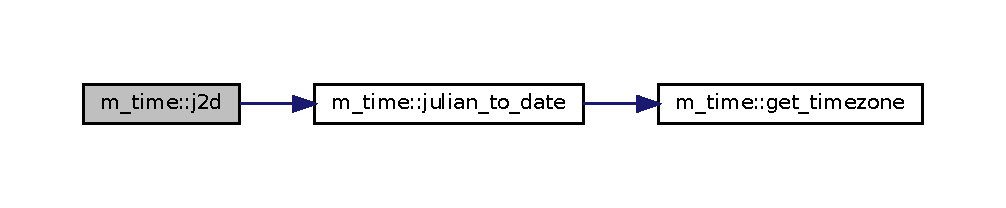
\includegraphics[width=350pt]{namespacem__time_a3ad5cad6df02c53e0429c3602a072e3c_cgraph}
\end{center}
\end{figure}
Here is the caller graph for this function\+:\nopagebreak
\begin{figure}[H]
\begin{center}
\leavevmode
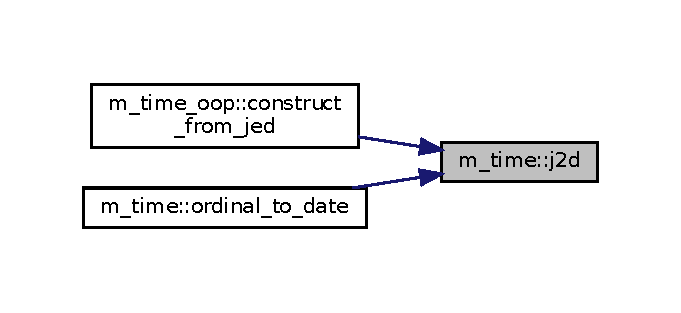
\includegraphics[width=327pt]{namespacem__time_a3ad5cad6df02c53e0429c3602a072e3c_icgraph}
\end{center}
\end{figure}
\mbox{\Hypertarget{namespacem__time_abb44cf18cd0a3e420c20469efb056203}\label{namespacem__time_abb44cf18cd0a3e420c20469efb056203}} 
\index{m\_time@{m\_time}!julian\_to\_date@{julian\_to\_date}}
\index{julian\_to\_date@{julian\_to\_date}!m\_time@{m\_time}}
\doxysubsubsection{\texorpdfstring{julian\_to\_date()}{julian\_to\_date()}}
{\footnotesize\ttfamily subroutine, public m\+\_\+time\+::julian\+\_\+to\+\_\+date (\begin{DoxyParamCaption}\item[{real(kind=\mbox{\hyperlink{namespacem__time_ac10ea9e8d59ec74eaa7d89f2517d7422}{realtime}}), intent(in)}]{julian,  }\item[{integer, dimension(8), intent(out)}]{dat,  }\item[{integer, intent(out)}]{ierr }\end{DoxyParamCaption})}

\hypertarget{namespacem__time_autotoc_md10}{}\doxysubsubsection{N\+A\+ME}\label{namespacem__time_autotoc_md10}
julian\+\_\+to\+\_\+date(3f) -\/ \mbox{[}M\+\_\+time\+:J\+U\+L\+I\+AN\mbox{]} converts a J\+ED(Julian Ephemeris Date) to a D\+AT date-\/time array. (L\+I\+C\+E\+N\+SE\+:PD)\hypertarget{namespacem__time_autotoc_md11}{}\doxysubsubsection{S\+Y\+N\+O\+P\+S\+IS}\label{namespacem__time_autotoc_md11}
\begin{DoxyVerb}subroutine julian_to_date(julian,dat,ierr)

 real(kind=realtime),intent(in) :: julian
 integer,intent(out)            :: dat(8)
 integer,intent(out)            :: ierr
\end{DoxyVerb}
\hypertarget{namespacem__time_autotoc_md12}{}\doxysubsubsection{D\+E\+S\+C\+R\+I\+P\+T\+I\+ON}\label{namespacem__time_autotoc_md12}
Converts a Unix Epoch Time (U\+ET) value to a D\+AT date-\/time array. U\+ET is the number of seconds since 00\+:00 on January 1st, 1970, U\+TC.\hypertarget{namespacem__time_autotoc_md13}{}\doxysubsubsection{O\+P\+T\+I\+O\+NS}\label{namespacem__time_autotoc_md13}
julian Julian Date (days) dat Integer array holding a \char`\"{}\+D\+A\+T\char`\"{} array, similar in structure to the array returned by the intrinsic D\+A\+T\+E\+\_\+\+A\+N\+D\+\_\+\+T\+I\+M\+E(3f)\+:

dat=\mbox{[} year,month,day,timezone,hour,\& \& minutes,seconds,milliseconds\mbox{]}\hypertarget{namespacem__time_autotoc_md14}{}\doxysubsubsection{R\+E\+T\+U\+R\+NS}\label{namespacem__time_autotoc_md14}
unixtime The \char`\"{}\+Unix Epoch\char`\"{} time, or the number of seconds since 00\+:00\+:00 on January 1st, 1970, U\+TC. ierr Error code. If 0 no error occurred.\hypertarget{namespacem__time_autotoc_md15}{}\doxysubsubsection{E\+X\+A\+M\+P\+LE}\label{namespacem__time_autotoc_md15}
\begin{DoxyVerb} Sample program:

  program demo_julian_to_date
  use M_time, only : julian_to_date, fmtdate, realtime
  implicit none
  real(kind=realtime)     :: juliandate
  integer                 :: dat(8)
  integer                 :: ierr
     ! set sample Julian Date
     juliandate=2457589.129d0
     ! create DAT array for this date
     call julian_to_date(juliandate,dat,ierr)
     write(*,*)'Sample Date=',fmtdate(dat)
     ! go back one day
     call julian_to_date(juliandate-1.0d0,dat,ierr)
     write(*,*)'Day Before =',fmtdate(dat)
     ! go forward one day
     call julian_to_date(juliandate+1.0d0,dat,ierr)
     write(*,*)'Day After  =',fmtdate(dat)
  end program demo_julian_to_date

 Results:

  Sample Date=Tuesday, July 19th, 2016 11:05:45 AM UTC-04:00
  Day Before =Monday, July 18th, 2016 11:05:45 AM UTC-04:00
  Day After  =Wednesday, July 20th, 2016 11:05:45 AM UTC-04:00
\end{DoxyVerb}
\hypertarget{namespacem__time_autotoc_md16}{}\doxysubsubsection{A\+U\+T\+H\+OR}\label{namespacem__time_autotoc_md16}
John S. Urban, 2015 \hypertarget{namespacem__time_autotoc_md17}{}\doxysubsubsection{L\+I\+C\+E\+N\+SE}\label{namespacem__time_autotoc_md17}
Public Domain 

References get\+\_\+timezone(), and secday.

Here is the call graph for this function\+:\nopagebreak
\begin{figure}[H]
\begin{center}
\leavevmode
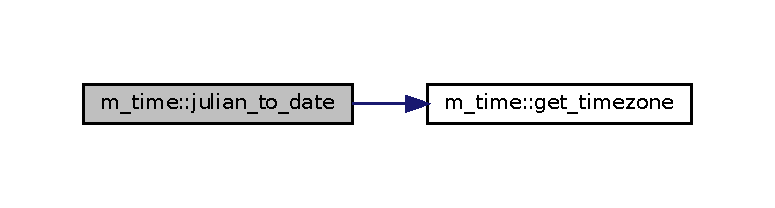
\includegraphics[width=350pt]{namespacem__time_abb44cf18cd0a3e420c20469efb056203_cgraph}
\end{center}
\end{figure}
Here is the caller graph for this function\+:\nopagebreak
\begin{figure}[H]
\begin{center}
\leavevmode
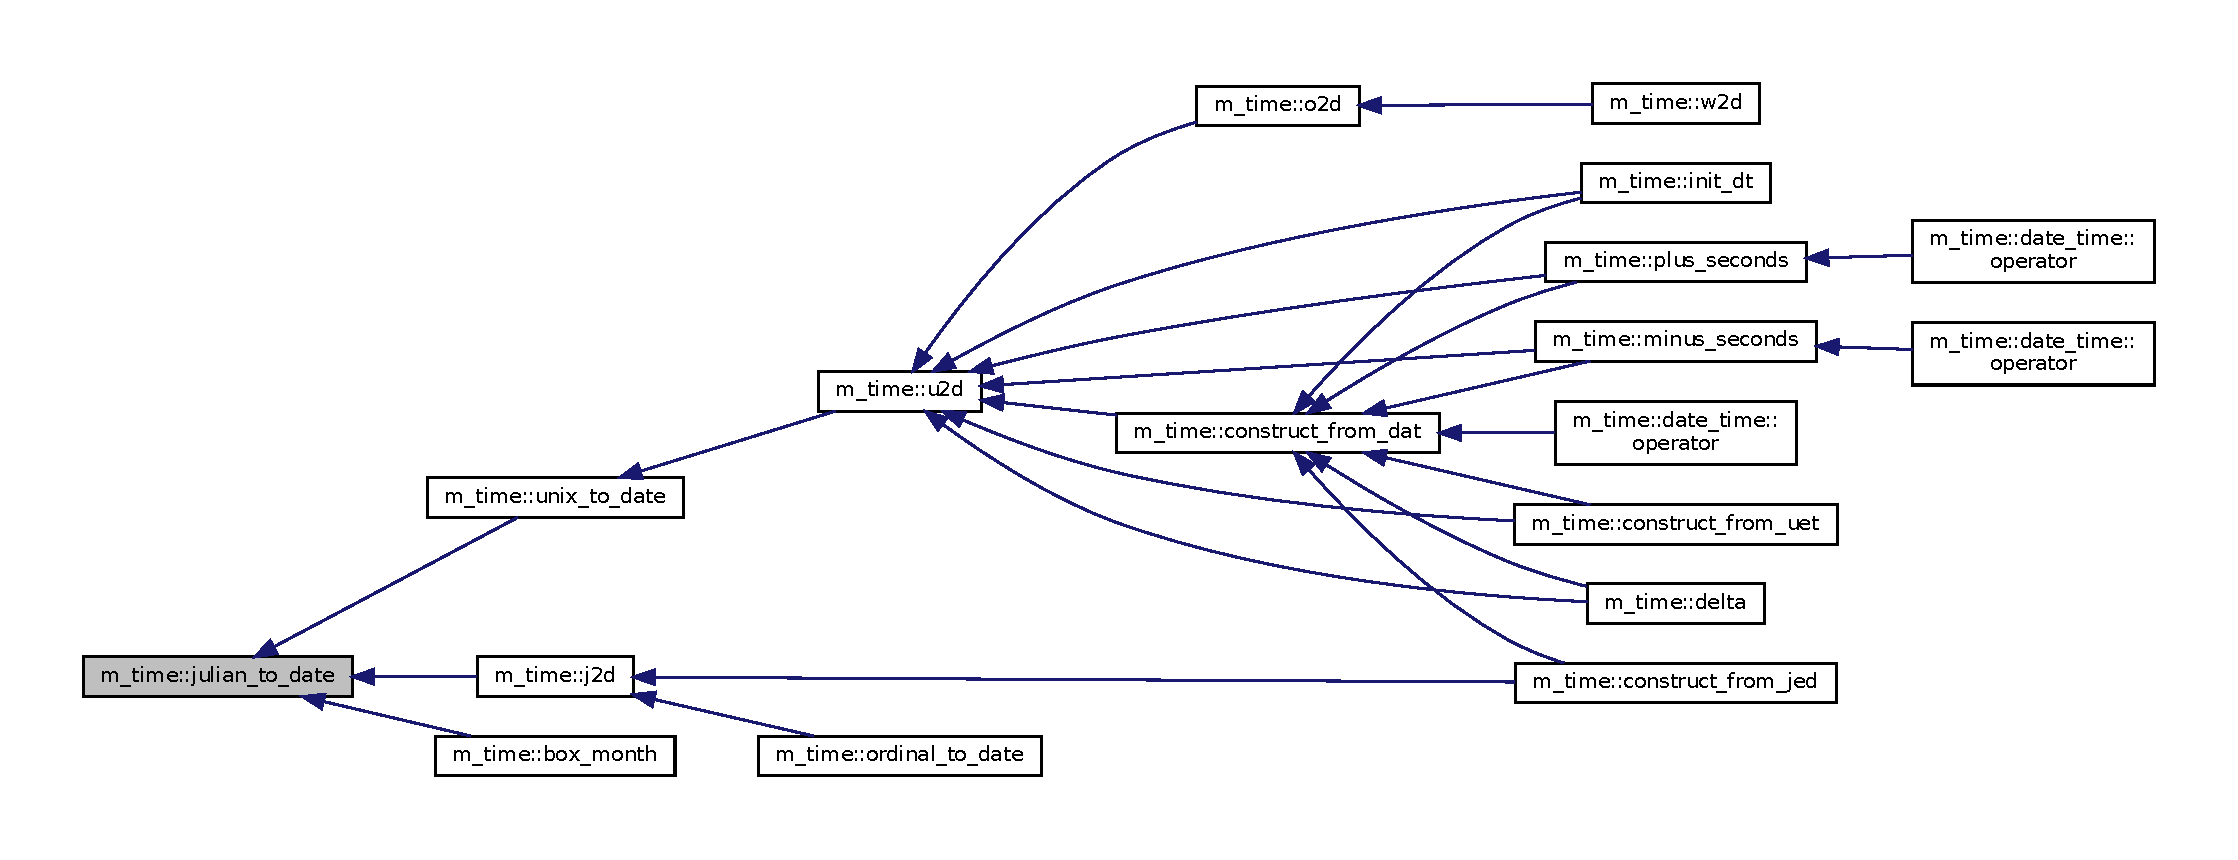
\includegraphics[width=350pt]{namespacem__time_abb44cf18cd0a3e420c20469efb056203_icgraph}
\end{center}
\end{figure}
\mbox{\Hypertarget{namespacem__time_a8188c7ed4e592c4f2388d28c75486726}\label{namespacem__time_a8188c7ed4e592c4f2388d28c75486726}} 
\index{m\_time@{m\_time}!mo2d@{mo2d}}
\index{mo2d@{mo2d}!m\_time@{m\_time}}
\doxysubsubsection{\texorpdfstring{mo2d()}{mo2d()}}
{\footnotesize\ttfamily integer function, dimension(8), public m\+\_\+time\+::mo2d (\begin{DoxyParamCaption}\item[{character(len=$\ast$), intent(in)}]{month\+\_\+name,  }\item[{integer, intent(in), optional}]{year }\end{DoxyParamCaption})}

\hypertarget{namespacem__time_autotoc_md70}{}\doxysubsubsection{N\+A\+ME}\label{namespacem__time_autotoc_md70}
mo2d(3f) -\/ \mbox{[}M\+\_\+time\+:M\+O\+N\+T\+H\+\_\+\+N\+A\+ME\mbox{]} given month name return D\+AT date-\/time array for beginning of that month in specified year (L\+I\+C\+E\+N\+SE\+:PD)\hypertarget{namespacem__time_autotoc_md71}{}\doxysubsubsection{S\+Y\+N\+O\+P\+S\+IS}\label{namespacem__time_autotoc_md71}
\begin{DoxyVerb}   function mo2d(month_name,year) result (dat)

    character(len=*),intent(in) :: month_name
    integer,intent(in),optional :: year
    integer                     :: dat(8)
\end{DoxyVerb}
\hypertarget{namespacem__time_autotoc_md72}{}\doxysubsubsection{D\+E\+S\+C\+R\+I\+P\+T\+I\+ON}\label{namespacem__time_autotoc_md72}
Given a Common Calendar month name, return the date as a \char`\"{}\+D\+A\+T\char`\"{} array for the 1st day of the month. An optional year may be specified. The year defaults to the current year.\hypertarget{namespacem__time_autotoc_md73}{}\doxysubsubsection{O\+P\+T\+I\+O\+NS}\label{namespacem__time_autotoc_md73}
month\+\_\+name A string representing a Common Calendar month name. year Optional year. Defaults to current year \hypertarget{namespacem__time_autotoc_md74}{}\doxysubsubsection{R\+E\+T\+U\+R\+NS}\label{namespacem__time_autotoc_md74}
dat An integer array that has the same structure as the array returned by the Fortran intrinsic D\+A\+T\+E\+\_\+\+A\+N\+D\+\_\+\+T\+I\+M\+E(3f)\+:

dat=\mbox{[} year,month,day,timezone,hour,\& \& minutes,seconds,milliseconds\mbox{]}\hypertarget{namespacem__time_autotoc_md75}{}\doxysubsubsection{E\+X\+A\+M\+P\+LE}\label{namespacem__time_autotoc_md75}
\begin{DoxyVerb}Sample program:

 program demo_mo2d
 use M_time, only : mo2d
 implicit none
    write(*,'(*(i0:,":"))')mo2d('March')
 end program demo_mo2d

results:

   2016:3:1:-240:0:0:0:0
\end{DoxyVerb}
\hypertarget{namespacem__time_autotoc_md76}{}\doxysubsubsection{A\+U\+T\+H\+OR}\label{namespacem__time_autotoc_md76}
John S. Urban, 2015 \hypertarget{namespacem__time_autotoc_md77}{}\doxysubsubsection{L\+I\+C\+E\+N\+SE}\label{namespacem__time_autotoc_md77}
Public Domain 

References mo2v(), and m\+\_\+time\+\_\+duplicate\+::stderr().

Here is the call graph for this function\+:\nopagebreak
\begin{figure}[H]
\begin{center}
\leavevmode
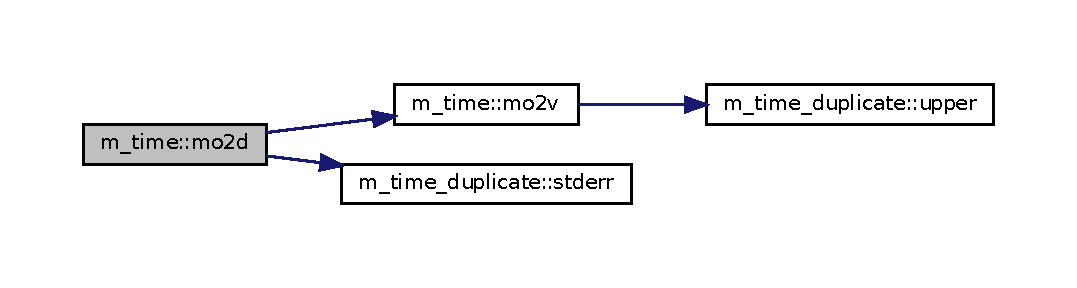
\includegraphics[width=350pt]{namespacem__time_a8188c7ed4e592c4f2388d28c75486726_cgraph}
\end{center}
\end{figure}
\mbox{\Hypertarget{namespacem__time_ad7bf0886754757e8961e562f06cf3bb7}\label{namespacem__time_ad7bf0886754757e8961e562f06cf3bb7}} 
\index{m\_time@{m\_time}!mo2v@{mo2v}}
\index{mo2v@{mo2v}!m\_time@{m\_time}}
\doxysubsubsection{\texorpdfstring{mo2v()}{mo2v()}}
{\footnotesize\ttfamily integer function, public m\+\_\+time\+::mo2v (\begin{DoxyParamCaption}\item[{character(len=$\ast$), intent(in)}]{month\+\_\+name }\end{DoxyParamCaption})}

\hypertarget{namespacem__time_autotoc_md78}{}\doxysubsubsection{N\+A\+ME}\label{namespacem__time_autotoc_md78}
mo2v(3f) -\/ \mbox{[}M\+\_\+time\+:M\+O\+N\+T\+H\+\_\+\+N\+A\+ME\mbox{]} given month name return month number (1-\/12) of that month (L\+I\+C\+E\+N\+SE\+:PD)\hypertarget{namespacem__time_autotoc_md79}{}\doxysubsubsection{S\+Y\+N\+O\+P\+S\+IS}\label{namespacem__time_autotoc_md79}
\begin{DoxyVerb}function mo2v(month_name) result(imonth)

  character(len=*),intent(in):: month_name ! month name
  integer                    :: imonth     ! month number
\end{DoxyVerb}
\hypertarget{namespacem__time_autotoc_md80}{}\doxysubsubsection{D\+E\+S\+C\+R\+I\+P\+T\+I\+ON}\label{namespacem__time_autotoc_md80}
Given a string representing the name or abbreviation of a Gregorian Calendar month return a number representing the position of the month in the calendar starting with 1 for January and ending with 12 for December.\hypertarget{namespacem__time_autotoc_md81}{}\doxysubsubsection{O\+P\+T\+I\+O\+NS}\label{namespacem__time_autotoc_md81}
month\+\_\+name name or abbreviation of month. Case is ignored Once enough characters are found to uniquely identify a month the rest of the name is ignored. \hypertarget{namespacem__time_autotoc_md82}{}\doxysubsubsection{R\+E\+T\+U\+R\+NS}\label{namespacem__time_autotoc_md82}
imonth month number returned. If the name is not recognized a -\/1 is returned.\hypertarget{namespacem__time_autotoc_md83}{}\doxysubsubsection{E\+X\+A\+M\+P\+LE}\label{namespacem__time_autotoc_md83}
\begin{DoxyVerb}Sample program:

 program demo_mo2v
 use M_time, only : mo2v
 implicit none
    write(*,*)mo2v("April")
    write(*,*)mo2v('Apr')
    ! NOTE: still matches September, as "SE" was enough
    write(*,*)mo2v('sexember')
    write(*,*)mo2v('unknown')  ! returns -1
 end program demo_mo2v

results:

   >  4
   >  4
   >  9
   > -1
\end{DoxyVerb}
\hypertarget{namespacem__time_autotoc_md84}{}\doxysubsubsection{A\+U\+T\+H\+OR}\label{namespacem__time_autotoc_md84}
John S. Urban, 2015 \hypertarget{namespacem__time_autotoc_md85}{}\doxysubsubsection{L\+I\+C\+E\+N\+SE}\label{namespacem__time_autotoc_md85}
Public Domain 

References m\+\_\+time\+\_\+duplicate\+::upper().

Here is the call graph for this function\+:\nopagebreak
\begin{figure}[H]
\begin{center}
\leavevmode
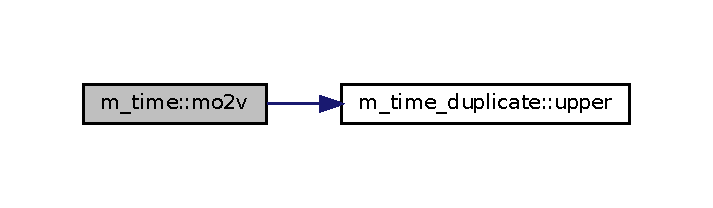
\includegraphics[width=342pt]{namespacem__time_ad7bf0886754757e8961e562f06cf3bb7_cgraph}
\end{center}
\end{figure}
Here is the caller graph for this function\+:\nopagebreak
\begin{figure}[H]
\begin{center}
\leavevmode
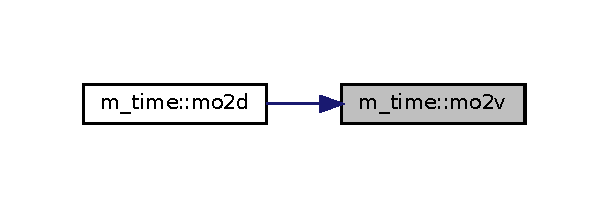
\includegraphics[width=292pt]{namespacem__time_ad7bf0886754757e8961e562f06cf3bb7_icgraph}
\end{center}
\end{figure}
\mbox{\Hypertarget{namespacem__time_a702b39998a769b8f60070c0bec975ee2}\label{namespacem__time_a702b39998a769b8f60070c0bec975ee2}} 
\index{m\_time@{m\_time}!moon\_fullness@{moon\_fullness}}
\index{moon\_fullness@{moon\_fullness}!m\_time@{m\_time}}
\doxysubsubsection{\texorpdfstring{moon\_fullness()}{moon\_fullness()}}
{\footnotesize\ttfamily integer function, public m\+\_\+time\+::moon\+\_\+fullness (\begin{DoxyParamCaption}\item[{integer, dimension(8), intent(in)}]{datin }\end{DoxyParamCaption})}

\hypertarget{namespacem__time_autotoc_md214}{}\doxysubsubsection{N\+A\+ME}\label{namespacem__time_autotoc_md214}
moon\+\_\+fullness(3f) -\/ \mbox{[}M\+\_\+time\+:A\+S\+T\+R\+O\+L\+O\+G\+I\+C\+AL\mbox{]} return percentage of moon phase from new to full (L\+I\+C\+E\+N\+SE\+:PD) \hypertarget{namespacem__time_autotoc_md215}{}\doxysubsubsection{S\+Y\+N\+O\+P\+S\+IS}\label{namespacem__time_autotoc_md215}
function moon\+\_\+fullness(datin)

integer,intent(in) \+:: datin(8) integer \+:: moon\+\_\+fullness\hypertarget{namespacem__time_autotoc_md216}{}\doxysubsubsection{D\+E\+S\+C\+R\+I\+P\+T\+I\+ON}\label{namespacem__time_autotoc_md216}
This procedure is used to support the P field descriptor for the fmtdate(3f) routine.

The moon circles the earth every 29.\+530588853 days on average, so pick a starting point and count. A new moon occurred at January 6, 2000, 18\+:14 U\+TC. Then it is easy to count the number of days since the last new moon. This is an approximate calculation.\hypertarget{namespacem__time_autotoc_md217}{}\doxysubsubsection{O\+P\+T\+I\+O\+NS}\label{namespacem__time_autotoc_md217}
datin D\+AT Date array describing input date\hypertarget{namespacem__time_autotoc_md218}{}\doxysubsubsection{R\+E\+S\+U\+L\+TS}\label{namespacem__time_autotoc_md218}
\begin{DoxyVerb} moon_fullness  0 is a new or dark moon, 100 is a full moon, + for waxing
                and - for waning.
\end{DoxyVerb}
\hypertarget{namespacem__time_autotoc_md219}{}\doxysubsubsection{E\+X\+A\+M\+P\+L\+ES}\label{namespacem__time_autotoc_md219}
\begin{DoxyVerb}Sample:

 program demo_moon_fullness
 use M_time, only : now
 use M_time, only : phase_of_moon
 use M_time, only : moon_fullness
 implicit none
 integer             :: dat(8)
    ! generate DAT array
    call date_and_time(values=dat)
    ! show DAT array
    write(*,'(" Today is:",*(i0:,":"))')dat
    ! the %p and %P fields are supported by fmtdate(3f)
    write(*,*)&
    &now('The phase of the moon is %p, with a fullness of %P')
    write(*,'(1x,*(a))',advance='no')&
    &'The phase of the moon is ',trim( phase_of_moon(dat)),','
    write(*,'(1x,a,i0,a)')&
    &'with a fullness of ', moon_fullness(dat),'%'
 end program demo_moon_fullness

Sample output:

  Today is:2018:11:3:-240:20:18:44:245
  The phase of the moon is Waning crescent, with a fullness of -30%
  The phase of the moon is Waning crescent, with a fullness of -30%
\end{DoxyVerb}
 \hypertarget{namespacem__time_autotoc_md220}{}\doxysubsubsection{A\+U\+T\+H\+OR}\label{namespacem__time_autotoc_md220}
John S. Urban, 2015 \hypertarget{namespacem__time_autotoc_md221}{}\doxysubsubsection{L\+I\+C\+E\+N\+SE}\label{namespacem__time_autotoc_md221}
Public Domain 

References d2j().

Here is the call graph for this function\+:\nopagebreak
\begin{figure}[H]
\begin{center}
\leavevmode
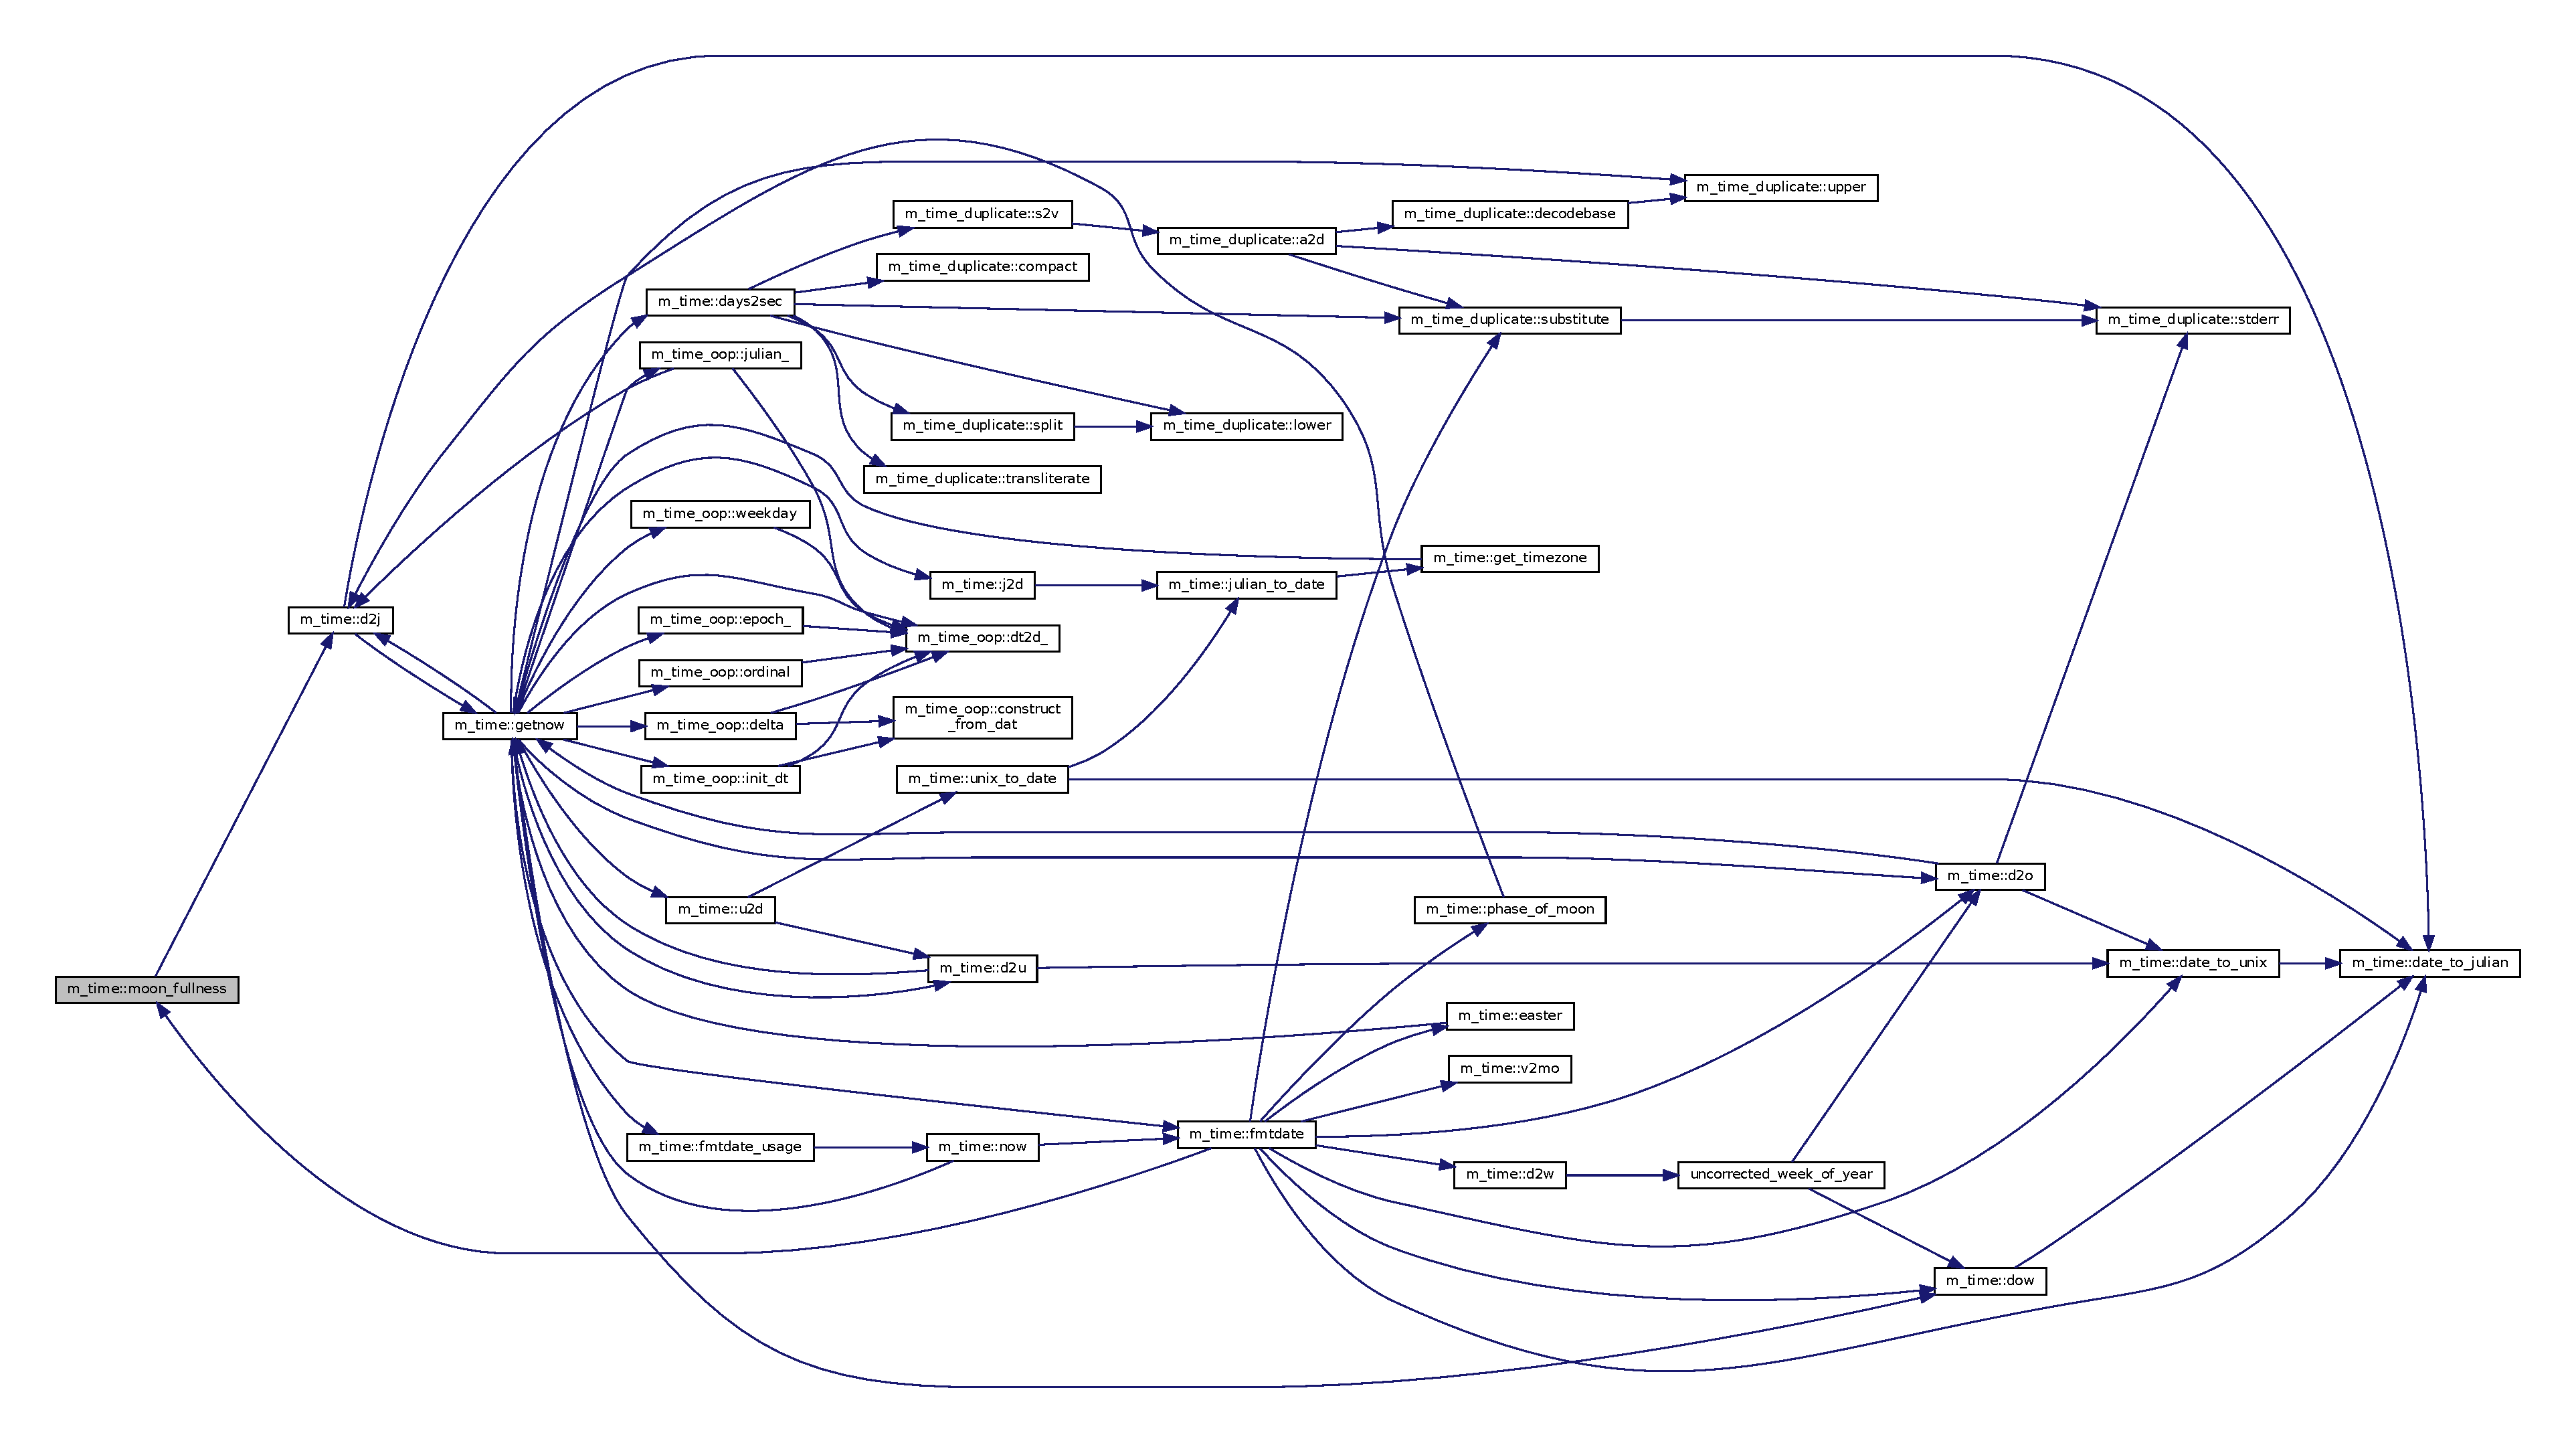
\includegraphics[width=350pt]{namespacem__time_a702b39998a769b8f60070c0bec975ee2_cgraph}
\end{center}
\end{figure}
Here is the caller graph for this function\+:\nopagebreak
\begin{figure}[H]
\begin{center}
\leavevmode
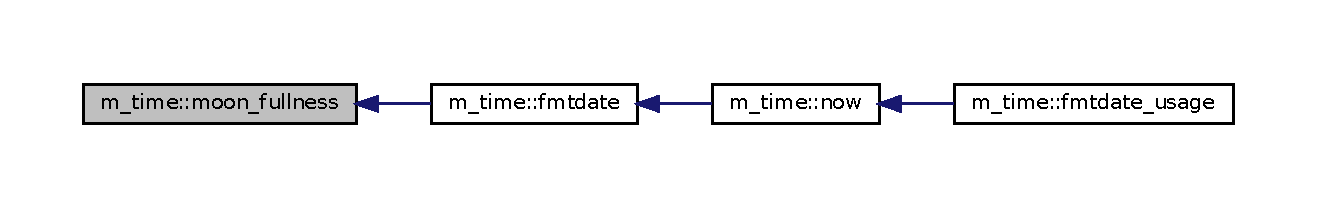
\includegraphics[width=350pt]{namespacem__time_a702b39998a769b8f60070c0bec975ee2_icgraph}
\end{center}
\end{figure}
\mbox{\Hypertarget{namespacem__time_a6b5e87be0e510ff268c1ecfbf67a3bdb}\label{namespacem__time_a6b5e87be0e510ff268c1ecfbf67a3bdb}} 
\index{m\_time@{m\_time}!now@{now}}
\index{now@{now}!m\_time@{m\_time}}
\doxysubsubsection{\texorpdfstring{now()}{now()}}
{\footnotesize\ttfamily character(len=\+:) function, allocatable, public m\+\_\+time\+::now (\begin{DoxyParamCaption}\item[{character(len=$\ast$), intent(in), optional}]{format }\end{DoxyParamCaption})}

\hypertarget{namespacem__time_autotoc_md86}{}\doxysubsubsection{N\+A\+ME}\label{namespacem__time_autotoc_md86}
now(3f) -\/ \mbox{[}M\+\_\+time\+:D\+A\+T\+E\+\_\+\+P\+R\+I\+N\+T\+I\+NG\mbox{]} return string representing current time given format (L\+I\+C\+E\+N\+SE\+:PD)\hypertarget{namespacem__time_autotoc_md87}{}\doxysubsubsection{S\+Y\+N\+O\+P\+S\+IS}\label{namespacem__time_autotoc_md87}
\begin{DoxyVerb}function now(format) RESULT (timestr)

 character(len=*),intent(in)     :: format  ! input format string
 character(len=:),allocatable    :: timestr ! formatted date
\end{DoxyVerb}
\hypertarget{namespacem__time_autotoc_md88}{}\doxysubsubsection{D\+E\+S\+C\+R\+I\+P\+T\+I\+ON}\label{namespacem__time_autotoc_md88}
The now(3f) function is a call to the fmtdate(3f) function using the current date and time. That is, it is a convenient way to print the current date and time.\hypertarget{namespacem__time_autotoc_md89}{}\doxysubsubsection{O\+P\+T\+I\+O\+NS}\label{namespacem__time_autotoc_md89}
format string describing how to format the current date and time. For a complete description of the formatting macros supported see fmtdate\+\_\+usage(3f). \hypertarget{namespacem__time_autotoc_md90}{}\doxysubsubsection{R\+E\+T\+U\+R\+NS}\label{namespacem__time_autotoc_md90}
timestr formatted output string representing date\hypertarget{namespacem__time_autotoc_md91}{}\doxysubsubsection{E\+X\+A\+M\+P\+LE}\label{namespacem__time_autotoc_md91}
\begin{DoxyVerb}Sample Program:

 program demo_now
 use M_time, only : now
 implicit none
    write(*,*)now("The current date is %w, %l %d, %Y %H:%m:%s %N")
    call showme()
 contains
 subroutine showme() ! see all formatting options
 use M_time, only : fmtdate_usage
    call fmtdate_usage() ! see all formatting options
 end subroutine
 end program demo_now

results:

   The current date is Sun, Jul 17th, 2016 01:21:35 PM
    ::
    :: description of all formatting options will appear here
    ::
\end{DoxyVerb}
\hypertarget{namespacem__time_autotoc_md92}{}\doxysubsubsection{A\+U\+T\+H\+OR}\label{namespacem__time_autotoc_md92}
John S. Urban, 2015 \hypertarget{namespacem__time_autotoc_md93}{}\doxysubsubsection{L\+I\+C\+E\+N\+SE}\label{namespacem__time_autotoc_md93}
Public Domain 

References fmtdate().

Here is the call graph for this function\+:\nopagebreak
\begin{figure}[H]
\begin{center}
\leavevmode
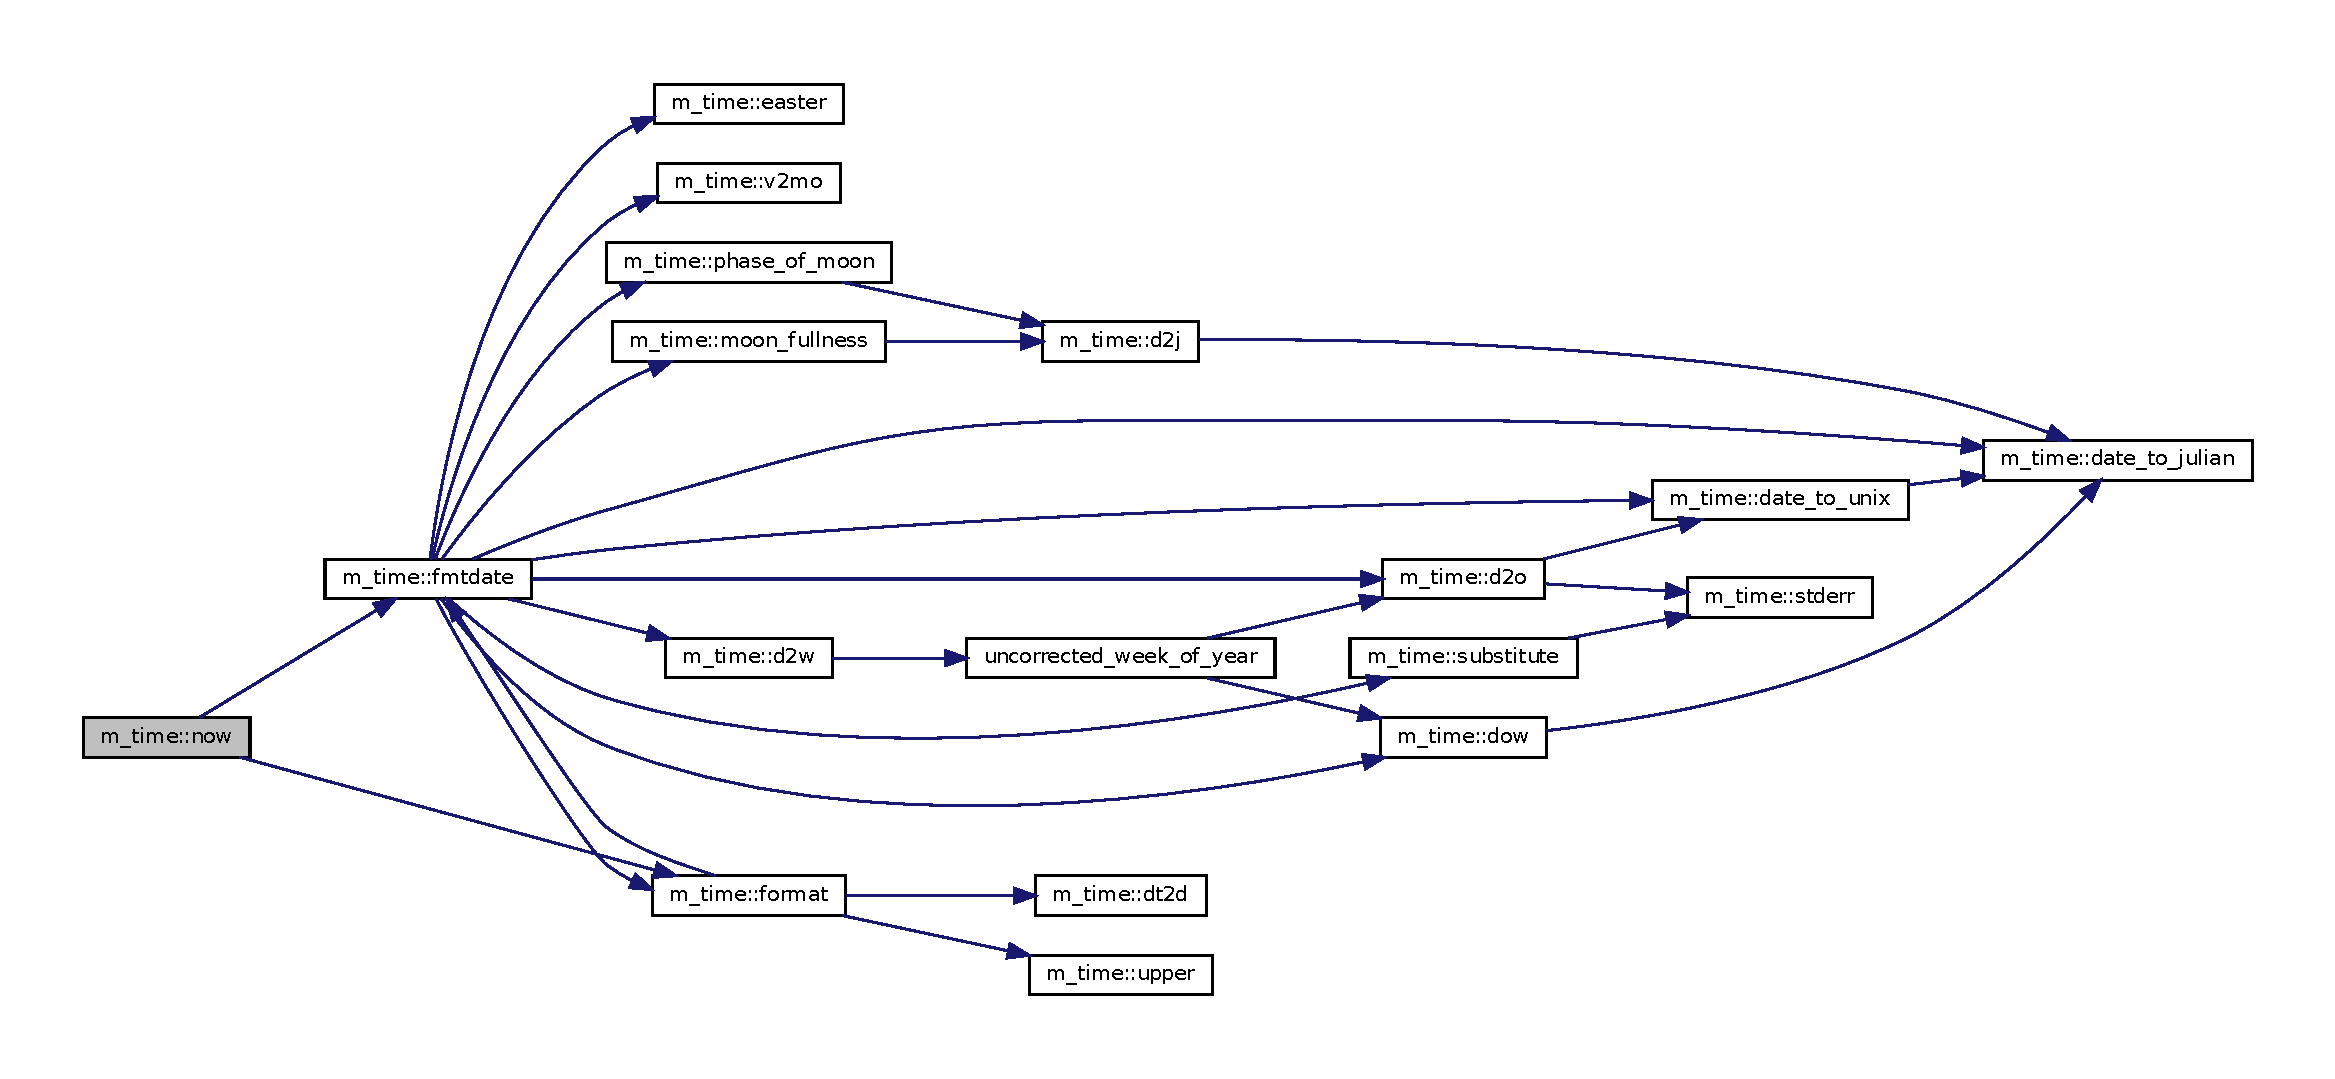
\includegraphics[width=350pt]{namespacem__time_a6b5e87be0e510ff268c1ecfbf67a3bdb_cgraph}
\end{center}
\end{figure}
Here is the caller graph for this function\+:\nopagebreak
\begin{figure}[H]
\begin{center}
\leavevmode
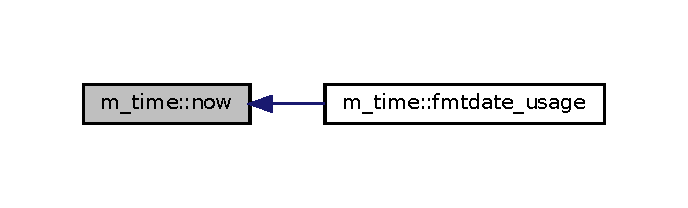
\includegraphics[width=330pt]{namespacem__time_a6b5e87be0e510ff268c1ecfbf67a3bdb_icgraph}
\end{center}
\end{figure}
\mbox{\Hypertarget{namespacem__time_a55e2cb9efc9d4d209ae2864f073d4f19}\label{namespacem__time_a55e2cb9efc9d4d209ae2864f073d4f19}} 
\index{m\_time@{m\_time}!o2d@{o2d}}
\index{o2d@{o2d}!m\_time@{m\_time}}
\doxysubsubsection{\texorpdfstring{o2d()}{o2d()}}
{\footnotesize\ttfamily integer function, dimension(8), public m\+\_\+time\+::o2d (\begin{DoxyParamCaption}\item[{integer, intent(in)}]{ordinal,  }\item[{integer, optional}]{year }\end{DoxyParamCaption})}

\hypertarget{namespacem__time_autotoc_md54}{}\doxysubsubsection{N\+A\+ME}\label{namespacem__time_autotoc_md54}
o2d(3f) -\/ \mbox{[}M\+\_\+time\+:O\+R\+D\+I\+N\+A\+L\+\_\+\+D\+AY\mbox{]} converts Ordinal day to D\+AT date-\/time array (L\+I\+C\+E\+N\+SE\+:PD)\hypertarget{namespacem__time_autotoc_md55}{}\doxysubsubsection{S\+Y\+N\+O\+P\+S\+IS}\label{namespacem__time_autotoc_md55}
\begin{DoxyVerb}function o2d(ordinal,[year]) result (dat)

 integer,intent(in) :: ordinal  ! the day of the year
 integer,optional   :: year     ! year
 integer            :: dat(8)   ! date time array
\end{DoxyVerb}
\hypertarget{namespacem__time_autotoc_md56}{}\doxysubsubsection{D\+E\+S\+C\+R\+I\+P\+T\+I\+ON}\label{namespacem__time_autotoc_md56}
Given an Ordinal day of the year return a date in the form of a \char`\"{}\+D\+A\+T\char`\"{} array.\hypertarget{namespacem__time_autotoc_md57}{}\doxysubsubsection{O\+P\+T\+I\+O\+NS}\label{namespacem__time_autotoc_md57}
ordinal The day of the year for the given year, where Jan 1st=1.

year An optional year for the ordinal day. If not present the current year is assumed.\hypertarget{namespacem__time_autotoc_md58}{}\doxysubsubsection{R\+E\+T\+U\+R\+NS}\label{namespacem__time_autotoc_md58}
dat Integer array holding a \char`\"{}\+D\+A\+T\char`\"{} array, similar in structure to the array returned by the intrinsic D\+A\+T\+E\+\_\+\+A\+N\+D\+\_\+\+T\+I\+M\+E(3f)\+:

dat=\mbox{[} year,month,day,timezone,hour,\& \& minutes,seconds,milliseconds\mbox{]}

The timezone value is from the current time on the current platform.\hypertarget{namespacem__time_autotoc_md59}{}\doxysubsubsection{E\+X\+A\+M\+P\+LE}\label{namespacem__time_autotoc_md59}
\begin{DoxyVerb}Sample program:

 program demo_o2d
 use M_time, only : o2d,fmtdate
 implicit none
 integer :: year
    do year=2004,2008
       write(*,*)&
       & '100th day of ',year,' is ',fmtdate(o2d(100,year))
    enddo
    write(*,*)'100th day of this year is ',fmtdate(o2d(100))
 end program demo_o2d

results:

 100th day of 2004 is Friday, April 9th, 2004 ...
 00:00:00 PM UTC-02:40
 100th day of 2005 is Sunday, April 10th, 2005 ...
 00:00:00 PM UTC-02:40
 100th day of 2006 is Monday, April 10th, 2006 ...
 00:00:00 PM UTC-02:40
 100th day of 2007 is Tuesday, April 10th, 2007 ...
 00:00:00 PM UTC-02:40
 100th day of 2008 is Wednesday, April 9th, 2008 ...
 00:00:00 PM UTC-02:40
 100th day of this year is Saturday, April 9th, 2016 ...
 00:00:00 PM UTC-02:40
\end{DoxyVerb}
 \hypertarget{namespacem__time_autotoc_md60}{}\doxysubsubsection{A\+U\+T\+H\+OR}\label{namespacem__time_autotoc_md60}
John S. Urban, 2015 \hypertarget{namespacem__time_autotoc_md61}{}\doxysubsubsection{L\+I\+C\+E\+N\+SE}\label{namespacem__time_autotoc_md61}
Public Domain 

References date\+\_\+to\+\_\+unix(), get\+\_\+timezone(), m\+\_\+time\+\_\+duplicate\+::stderr(), and u2d().

Here is the call graph for this function\+:\nopagebreak
\begin{figure}[H]
\begin{center}
\leavevmode
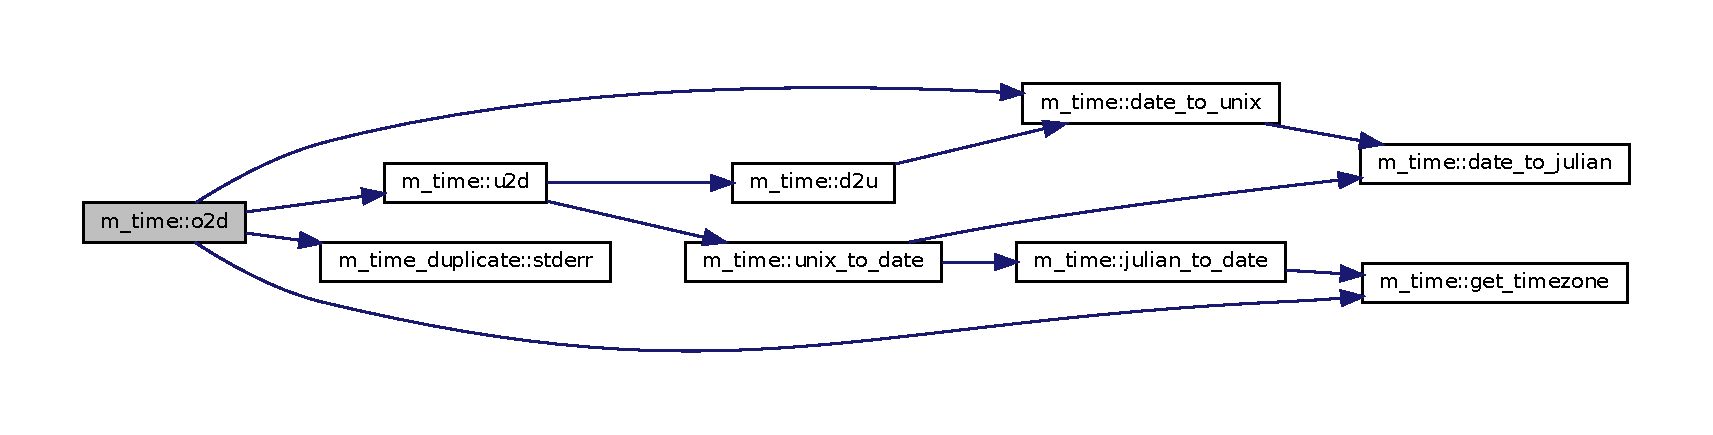
\includegraphics[width=350pt]{namespacem__time_a55e2cb9efc9d4d209ae2864f073d4f19_cgraph}
\end{center}
\end{figure}
Here is the caller graph for this function\+:\nopagebreak
\begin{figure}[H]
\begin{center}
\leavevmode
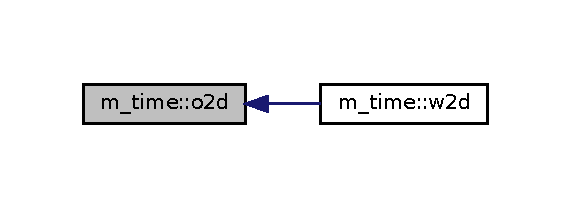
\includegraphics[width=274pt]{namespacem__time_a55e2cb9efc9d4d209ae2864f073d4f19_icgraph}
\end{center}
\end{figure}
\mbox{\Hypertarget{namespacem__time_ab8960d2aa60e134bcf77247d8b257963}\label{namespacem__time_ab8960d2aa60e134bcf77247d8b257963}} 
\index{m\_time@{m\_time}!ordinal\_seconds@{ordinal\_seconds}}
\index{ordinal\_seconds@{ordinal\_seconds}!m\_time@{m\_time}}
\doxysubsubsection{\texorpdfstring{ordinal\_seconds()}{ordinal\_seconds()}}
{\footnotesize\ttfamily integer function, public m\+\_\+time\+::ordinal\+\_\+seconds}

\hypertarget{namespacem__time_autotoc_md42}{}\doxysubsubsection{N\+A\+ME}\label{namespacem__time_autotoc_md42}
ordinal\+\_\+seconds(3f) -\/ \mbox{[}M\+\_\+time\+:O\+R\+D\+I\+N\+A\+L\+\_\+\+D\+AY\mbox{]} seconds since beginning of year (L\+I\+C\+E\+N\+SE\+:PD) \hypertarget{namespacem__time_autotoc_md43}{}\doxysubsubsection{S\+Y\+N\+O\+P\+S\+IS}\label{namespacem__time_autotoc_md43}
\begin{DoxyVerb}function ordinal_seconds()

 integer :: ordinal_seconds
\end{DoxyVerb}
 \hypertarget{namespacem__time_autotoc_md44}{}\doxysubsubsection{D\+E\+S\+C\+R\+I\+P\+T\+I\+ON}\label{namespacem__time_autotoc_md44}
Return number of seconds since beginning of current year.

Before using this routine consider the consequences if the application is running at the moment a new year begins.\hypertarget{namespacem__time_autotoc_md45}{}\doxysubsubsection{E\+X\+A\+M\+P\+LE}\label{namespacem__time_autotoc_md45}
\begin{DoxyVerb}sample program

 program demo_ordinal_seconds
 use M_time, only : ordinal_seconds
 implicit none
 character(len=1) :: paws
 integer          :: ios
 integer          :: istart, iend
 istart=ordinal_seconds()
 write(*,'(a)',advance='no')'now pause. Enter return to continue ...'
 read(*,'(a)',iostat=ios) paws
 iend=ordinal_seconds()
 write(*,*)'that took ',iend-istart,'seconds'
 write(*,*)istart,iend
 end program demo_ordinal_seconds
\end{DoxyVerb}
 \hypertarget{namespacem__time_autotoc_md46}{}\doxysubsubsection{A\+U\+T\+H\+OR}\label{namespacem__time_autotoc_md46}
John S. Urban, 2015 \hypertarget{namespacem__time_autotoc_md47}{}\doxysubsubsection{L\+I\+C\+E\+N\+SE}\label{namespacem__time_autotoc_md47}
Public Domain 

References d2o().

Here is the call graph for this function\+:\nopagebreak
\begin{figure}[H]
\begin{center}
\leavevmode
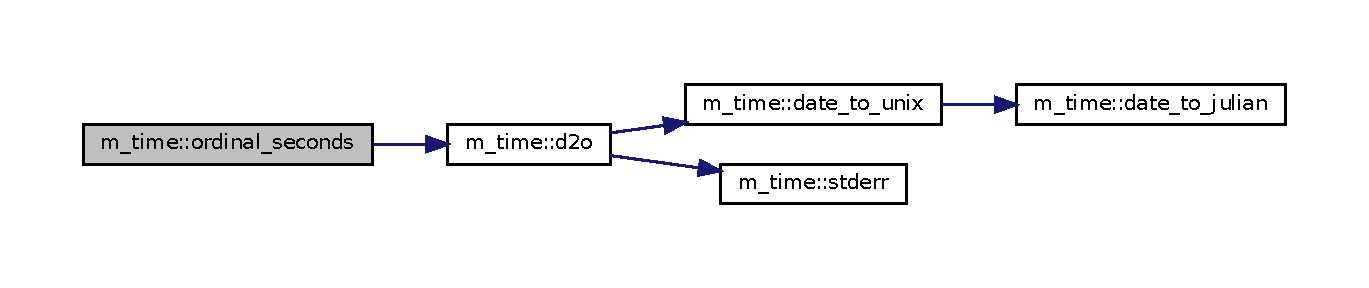
\includegraphics[width=350pt]{namespacem__time_ab8960d2aa60e134bcf77247d8b257963_cgraph}
\end{center}
\end{figure}
\mbox{\Hypertarget{namespacem__time_aa4dca4409bf20a011bb04988c1335d63}\label{namespacem__time_aa4dca4409bf20a011bb04988c1335d63}} 
\index{m\_time@{m\_time}!ordinal\_to\_date@{ordinal\_to\_date}}
\index{ordinal\_to\_date@{ordinal\_to\_date}!m\_time@{m\_time}}
\doxysubsubsection{\texorpdfstring{ordinal\_to\_date()}{ordinal\_to\_date()}}
{\footnotesize\ttfamily subroutine, public m\+\_\+time\+::ordinal\+\_\+to\+\_\+date (\begin{DoxyParamCaption}\item[{integer}]{yyyy,  }\item[{integer}]{ddd,  }\item[{integer, dimension(8)}]{dat }\end{DoxyParamCaption})}

\hypertarget{namespacem__time_autotoc_md48}{}\doxysubsubsection{N\+A\+ME}\label{namespacem__time_autotoc_md48}
ordinal\+\_\+to\+\_\+date(3f) -\/ \mbox{[}M\+\_\+time\+:O\+R\+D\+I\+N\+A\+L\+\_\+\+D\+AY\mbox{]} when given a valid year and day of the year returns the D\+AT array for the date (L\+I\+C\+E\+N\+SE\+:PD) \hypertarget{namespacem__time_autotoc_md49}{}\doxysubsubsection{S\+Y\+N\+O\+P\+S\+IS}\label{namespacem__time_autotoc_md49}
\begin{DoxyVerb}  subroutine ordinal_to_date(yyyy, ddd, dat)

   integer, intent(in)   :: yyyy
   integer, intent(in)   :: ddd
   integer, intent(out)  :: dat
\end{DoxyVerb}
 \hypertarget{namespacem__time_autotoc_md50}{}\doxysubsubsection{D\+E\+S\+C\+R\+I\+P\+T\+I\+ON}\label{namespacem__time_autotoc_md50}
When given a valid year, Y\+Y\+YY, and day of the year, D\+DD, returns the date as a D\+AT date array \hypertarget{namespacem__time_autotoc_md51}{}\doxysubsubsection{O\+P\+T\+I\+O\+NS}\label{namespacem__time_autotoc_md51}
yyyy known year ddd known ordinal day of the year \hypertarget{namespacem__time_autotoc_md52}{}\doxysubsubsection{R\+E\+T\+U\+R\+NS}\label{namespacem__time_autotoc_md52}
dat D\+AT array describing the date \hypertarget{namespacem__time_autotoc_md53}{}\doxysubsubsection{E\+X\+A\+M\+P\+LE}\label{namespacem__time_autotoc_md53}
\begin{DoxyVerb}Sample program:

 program demo_ordinal_to_date
 use M_time, only : ordinal_to_date
 implicit none
 INTEGER            :: yyyy, ddd, mm, dd, yy
 integer            :: dat(8)
 integer            :: ios
   INFINITE: do
      write(*,'(a)',advance='no')&
      & 'Enter year YYYY and ordinal day of year DD '
      read(*,*,iostat=ios)yyyy,ddd
      if(ios.ne.0)exit INFINITE
      ! recover month and day from year and day number.
      call ordinal_to_date(yyyy, ddd, dat)
      yy=dat(1)
      mm=dat(2)
      dd=dat(3)
      write(*,'(*(g0))')'For Year ',yyyy,' and Ordinal day ',ddd,  &
      &         ' Month is ',mm,' and Day of Month is ',dd, &
      &         ' and Year is ',yy
    enddo INFINITE
 end program demo_ordinal_to_date
\end{DoxyVerb}
 

References d2j(), j2d(), and realtime.

Here is the call graph for this function\+:\nopagebreak
\begin{figure}[H]
\begin{center}
\leavevmode
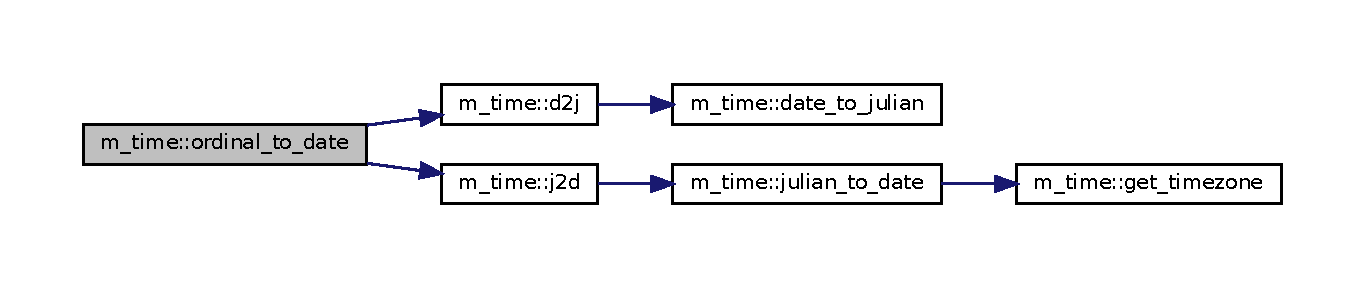
\includegraphics[width=350pt]{namespacem__time_aa4dca4409bf20a011bb04988c1335d63_cgraph}
\end{center}
\end{figure}
\mbox{\Hypertarget{namespacem__time_ab8a976e2f113cc38b6df80974cee55dc}\label{namespacem__time_ab8a976e2f113cc38b6df80974cee55dc}} 
\index{m\_time@{m\_time}!phase\_of\_moon@{phase\_of\_moon}}
\index{phase\_of\_moon@{phase\_of\_moon}!m\_time@{m\_time}}
\doxysubsubsection{\texorpdfstring{phase\_of\_moon()}{phase\_of\_moon()}}
{\footnotesize\ttfamily character(len=\+:) function, allocatable, public m\+\_\+time\+::phase\+\_\+of\+\_\+moon (\begin{DoxyParamCaption}\item[{integer, dimension(8), intent(in)}]{datin }\end{DoxyParamCaption})}

\hypertarget{namespacem__time_autotoc_md208}{}\doxysubsubsection{N\+A\+ME}\label{namespacem__time_autotoc_md208}
phase\+\_\+of\+\_\+moon(3f) -\/ \mbox{[}M\+\_\+time\+:A\+S\+T\+R\+O\+L\+O\+G\+I\+C\+AL\mbox{]} return name for phase of moon for given date (L\+I\+C\+E\+N\+SE\+:PD) \hypertarget{namespacem__time_autotoc_md209}{}\doxysubsubsection{S\+Y\+N\+O\+P\+S\+IS}\label{namespacem__time_autotoc_md209}
function phase\+\_\+of\+\_\+moon(datin)

integer,intent(in) \+:: datin(8) character(len=\+:),allocatable \+:: phase\+\_\+of\+\_\+moon\hypertarget{namespacem__time_autotoc_md210}{}\doxysubsubsection{D\+E\+S\+C\+R\+I\+P\+T\+I\+ON}\label{namespacem__time_autotoc_md210}
Phases Of The Moon

This procedure is used to support the p field descriptor for the fmtdate(3f) routine.

The moon circles the earth every 29.\+530588853 days on average, so pick a starting point and count. A new moon occurred at Julian date 2451550.\+1 (January 6, 2000, 18\+:14 U\+TC). Then it is easy to count the number of days since the last new moon. This is an approximate calculation.

There are eight generally recognized phases of the moon in common use

o new or dark o waxing crescent o first quarter o waxing gibbous o full o waning gibbous o last quarter o waning crescent

To calculate the phase of the moon simply divide the days since the last new moon by eight and select the appropriate phase.

Note that technically the four states (new, first quarter, full, third quarter) are events not phases. That is to say, the moon is technically only new for an instant.\hypertarget{namespacem__time_autotoc_md211}{}\doxysubsubsection{E\+X\+A\+M\+P\+L\+ES}\label{namespacem__time_autotoc_md211}
Sample\+:

program demo\+\_\+phase\+\_\+of\+\_\+moon use M\+\_\+time, only \+: now use M\+\_\+time, only \+: phase\+\_\+of\+\_\+moon use M\+\_\+time, only \+: moon\+\_\+fullness implicit none integer \+:: dat(8) ! generate D\+AT array call date\+\_\+and\+\_\+time(values=dat) ! show D\+AT array write($\ast$,\textquotesingle{}(\char`\"{} Today is\+:\char`\"{},$\ast$(i0\+:,\char`\"{}\+:\char`\"{}))\textquotesingle{})dat ! the p and P fields are supported by fmtdate(3f) write($\ast$,$\ast$)\& \& now(\textquotesingle{}The phase of the moon is p, with a fullness of P\textquotesingle{}) write($\ast$,\textquotesingle{}(1x,$\ast$(a))\textquotesingle{},advance=\textquotesingle{}no\textquotesingle{})\& \& \textquotesingle{}The phase of the moon is \textquotesingle{},trim( phase\+\_\+of\+\_\+moon(dat)),\textquotesingle{},\textquotesingle{} write($\ast$,\textquotesingle{}(1x,a,i0,a)\textquotesingle{})\textquotesingle{}with a fullness of \textquotesingle{},moon\+\_\+fullness(dat),\textquotesingle{}\textquotesingle{} end program demo\+\_\+phase\+\_\+of\+\_\+moon

Sample output\+:

Today is\+:2018\+:11\+:3\+:-\/240\+:20\+:18\+:44\+:245 The phase of the moon is Waning crescent, with a fullness of -\/30\% The phase of the moon is Waning crescent, with a fullness of -\/30\%\hypertarget{namespacem__time_autotoc_md212}{}\doxysubsubsection{A\+U\+T\+H\+OR}\label{namespacem__time_autotoc_md212}
John S. Urban, 2015 \hypertarget{namespacem__time_autotoc_md213}{}\doxysubsubsection{L\+I\+C\+E\+N\+SE}\label{namespacem__time_autotoc_md213}
Public Domain 

References d2j().

Here is the call graph for this function\+:\nopagebreak
\begin{figure}[H]
\begin{center}
\leavevmode
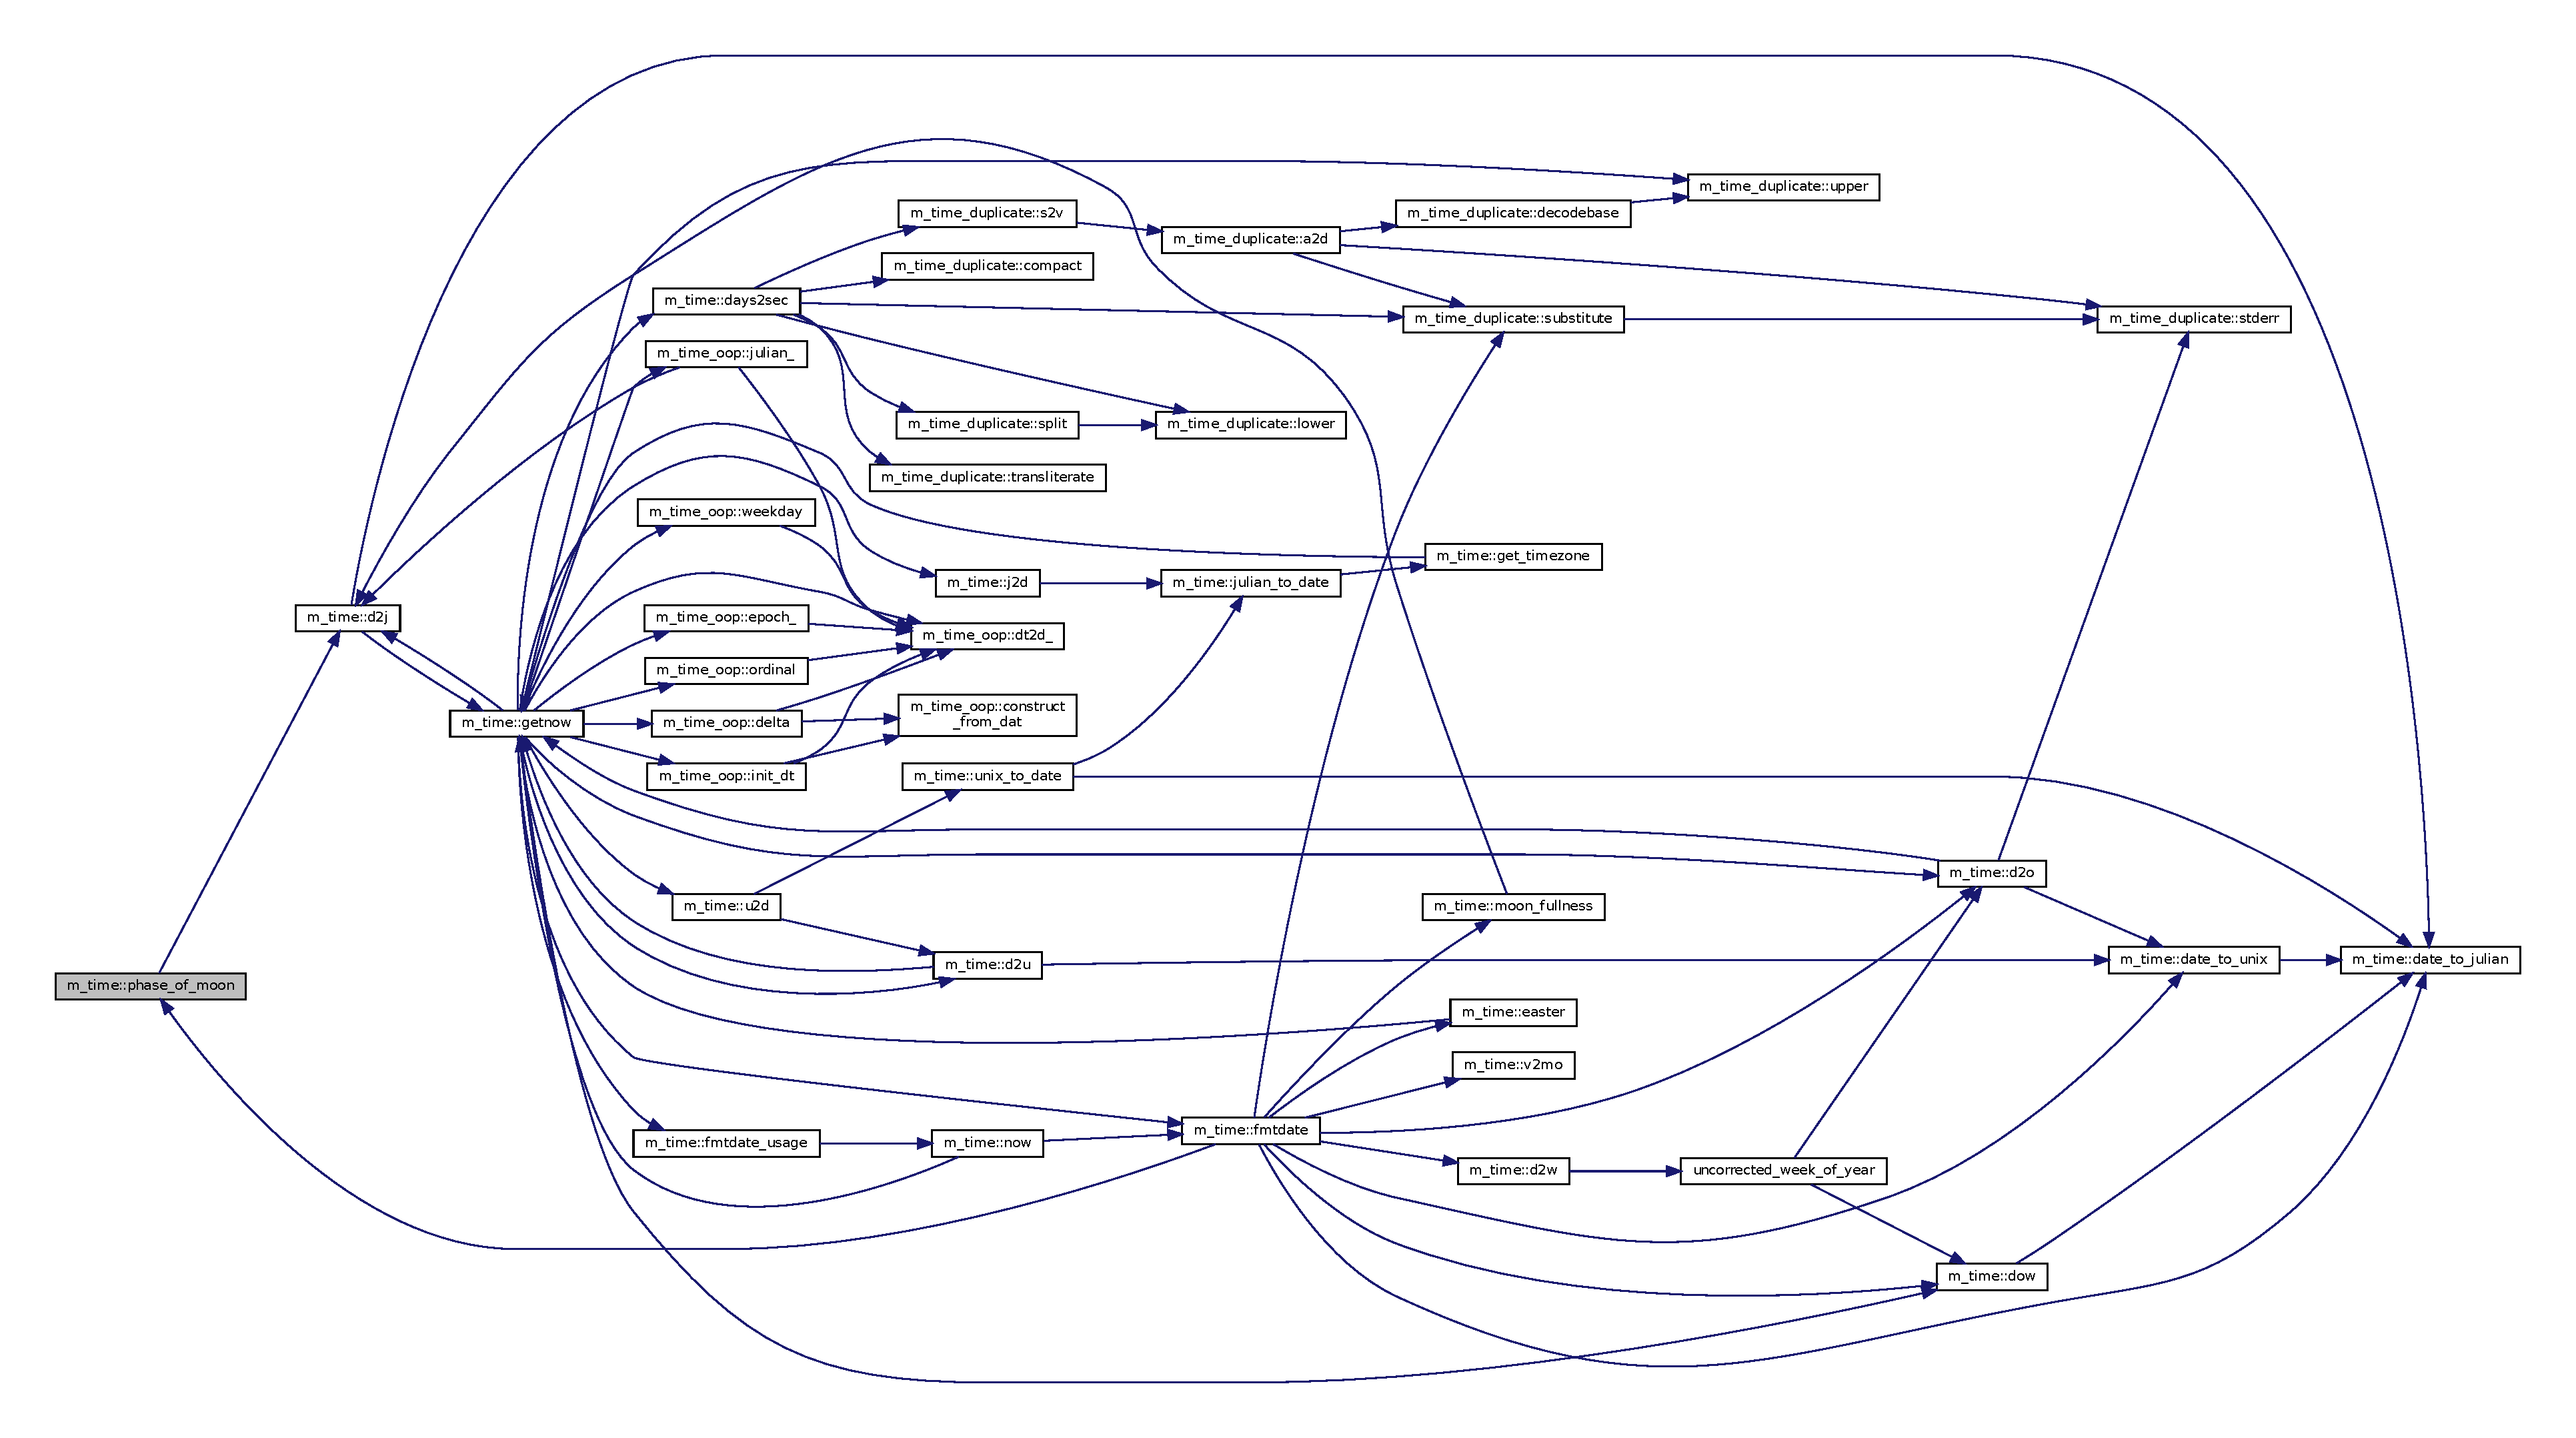
\includegraphics[width=350pt]{namespacem__time_ab8a976e2f113cc38b6df80974cee55dc_cgraph}
\end{center}
\end{figure}
Here is the caller graph for this function\+:\nopagebreak
\begin{figure}[H]
\begin{center}
\leavevmode
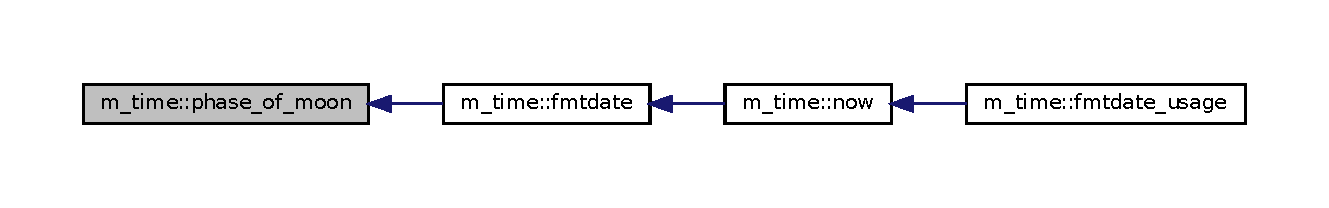
\includegraphics[width=350pt]{namespacem__time_ab8a976e2f113cc38b6df80974cee55dc_icgraph}
\end{center}
\end{figure}
\mbox{\Hypertarget{namespacem__time_a7788285d79b8d58323b05e9a30a2d992}\label{namespacem__time_a7788285d79b8d58323b05e9a30a2d992}} 
\index{m\_time@{m\_time}!sec2days@{sec2days}}
\index{sec2days@{sec2days}!m\_time@{m\_time}}
\doxysubsubsection{\texorpdfstring{sec2days()}{sec2days()}}
{\footnotesize\ttfamily character(len=\+:) function, allocatable, public m\+\_\+time\+::sec2days (\begin{DoxyParamCaption}\item[{class($\ast$), intent(in)}]{seconds,  }\item[{logical, intent(in), optional}]{crop }\end{DoxyParamCaption})}

\hypertarget{namespacem__time_autotoc_md192}{}\doxysubsubsection{N\+A\+ME}\label{namespacem__time_autotoc_md192}
sec2days(3f) -\/ \mbox{[}M\+\_\+time\+:D\+U\+R\+A\+T\+I\+ON\mbox{]} convert seconds to string of form dd-\/hh\+:mm\+:ss (L\+I\+C\+E\+N\+SE\+:PD)\hypertarget{namespacem__time_autotoc_md193}{}\doxysubsubsection{S\+Y\+N\+O\+P\+S\+IS}\label{namespacem__time_autotoc_md193}
\begin{DoxyVerb}function sec2days(seconds,crop) result(dhms)

 real(kind=realtime),intent(in) :: seconds
   or
 integer,intent(in)             :: seconds
   or
 real,intent(in)                :: seconds
   or
 character(len=*)               :: seconds

 logical,intent(in),optional    :: crop
 character(len=:),allocatable   :: dhms
\end{DoxyVerb}
\hypertarget{namespacem__time_autotoc_md194}{}\doxysubsubsection{D\+E\+S\+C\+R\+I\+P\+T\+I\+ON}\label{namespacem__time_autotoc_md194}
Given a number of seconds convert it to a string of the form \begin{DoxyVerb}dd-hh:mm:ss
\end{DoxyVerb}


where dd is days, hh hours, mm minutes and ss seconds.\hypertarget{namespacem__time_autotoc_md195}{}\doxysubsubsection{O\+P\+T\+I\+O\+NS}\label{namespacem__time_autotoc_md195}
seconds number of seconds to convert to string of form dd-\/hh\+:mm\+:ss. May be of type I\+N\+T\+E\+G\+ER, R\+E\+AL, R\+E\+AL(K\+I\+ND=R\+E\+A\+L\+T\+I\+ME), or C\+H\+A\+R\+A\+C\+T\+ER.

C\+H\+A\+R\+A\+C\+T\+ER strings may be of the form \mbox{[}N\+Nd\mbox{]}\mbox{[}N\+Nh\mbox{]}\mbox{[}N\+Nm\mbox{]}\mbox{[}N\+Ns\mbox{]}\mbox{[}N\+Nw\mbox{]}. Case,spaces and underscores are ignored. Allowed aliases for d,h,m, and s units are \begin{DoxyVerb}d -  days,day
m -  minutes,minute,min
h -  hours,hour,hrs,hr
s -  seconds,second,sec
\end{DoxyVerb}


The numeric values may represent floating point numbers.

crop if .true., remove leading zero day values or day and hour values. Optional, defaults to .false. . \hypertarget{namespacem__time_autotoc_md196}{}\doxysubsubsection{R\+E\+T\+U\+R\+NS}\label{namespacem__time_autotoc_md196}
dmhs the returned string of form \mbox{[}d\+:h\+:\mbox{]}m\+:s\hypertarget{namespacem__time_autotoc_md197}{}\doxysubsubsection{E\+X\+A\+M\+P\+LE}\label{namespacem__time_autotoc_md197}
\begin{DoxyVerb}Sample Program:

 program demo_sec2days
 use M_time, only : sec2days
 implicit none
    write(*,*)sec2days(129860)
    write(*,*)sec2days(80000.0d0)
    write(*,*)sec2days(80000.0,crop=.true.)
    write(*,*)sec2days('1 day 2.0hr 100 min 300.0seconds')
 end program demo_sec2days

results:

 1-12:04:20
 0-22:13:20
 22:13:20
 1-03:45:00
\end{DoxyVerb}
\hypertarget{namespacem__time_autotoc_md198}{}\doxysubsubsection{A\+U\+T\+H\+OR}\label{namespacem__time_autotoc_md198}
John S. Urban, 2015 \hypertarget{namespacem__time_autotoc_md199}{}\doxysubsubsection{L\+I\+C\+E\+N\+SE}\label{namespacem__time_autotoc_md199}
Public Domain 

References m\+\_\+time\+\_\+duplicate\+::compact(), m\+\_\+time\+\_\+duplicate\+::lower(), realtime, m\+\_\+time\+\_\+duplicate\+::s2v(), m\+\_\+time\+\_\+duplicate\+::split(), m\+\_\+time\+\_\+duplicate\+::substitute(), and m\+\_\+time\+\_\+duplicate\+::transliterate().

Here is the call graph for this function\+:\nopagebreak
\begin{figure}[H]
\begin{center}
\leavevmode
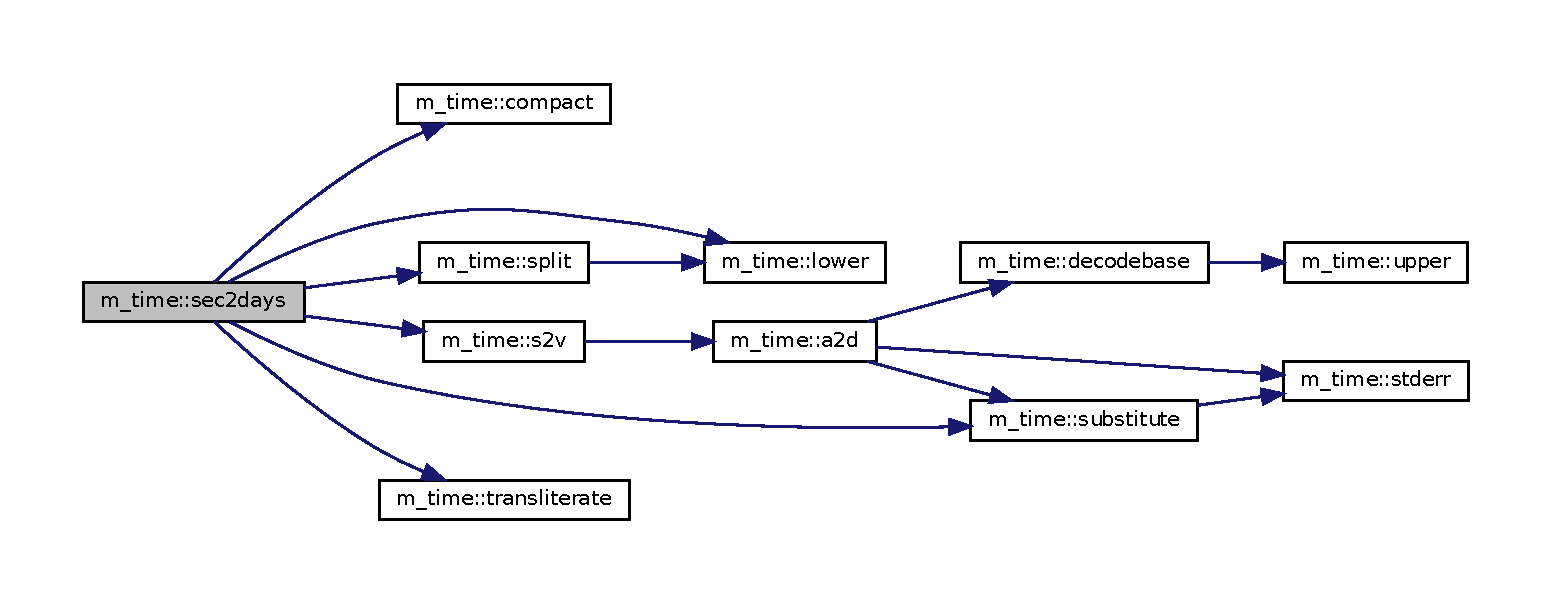
\includegraphics[width=350pt]{namespacem__time_a7788285d79b8d58323b05e9a30a2d992_cgraph}
\end{center}
\end{figure}
\mbox{\Hypertarget{namespacem__time_a7c5d028ae1e1e01162ffc7bb55dcbbb1}\label{namespacem__time_a7c5d028ae1e1e01162ffc7bb55dcbbb1}} 
\index{m\_time@{m\_time}!system\_sleep@{system\_sleep}}
\index{system\_sleep@{system\_sleep}!m\_time@{m\_time}}
\doxysubsubsection{\texorpdfstring{system\_sleep()}{system\_sleep()}}
{\footnotesize\ttfamily subroutine, public m\+\_\+time\+::system\+\_\+sleep (\begin{DoxyParamCaption}\item[{class($\ast$), intent(in)}]{seconds }\end{DoxyParamCaption})}

\hypertarget{namespacem__time_autotoc_md228}{}\doxysubsubsection{N\+A\+ME}\label{namespacem__time_autotoc_md228}
system\+\_\+sleep(3f) -\/ \mbox{[}M\+\_\+time\+:C\+\_\+\+I\+N\+T\+E\+R\+F\+A\+CE\mbox{]} call C sleep(3c) or usleep(3c) procedure (L\+I\+C\+E\+N\+SE\+:PD) \hypertarget{namespacem__time_autotoc_md229}{}\doxysubsubsection{S\+Y\+N\+O\+P\+S\+IS}\label{namespacem__time_autotoc_md229}
\begin{DoxyVerb}subroutine system_sleep(wait_seconds)

   integer,intent(in)  :: wait_seconds
      or
   real,intent(in)  :: wait_seconds
\end{DoxyVerb}
\hypertarget{namespacem__time_autotoc_md230}{}\doxysubsubsection{D\+E\+S\+C\+R\+I\+P\+T\+I\+ON}\label{namespacem__time_autotoc_md230}
The system\+\_\+sleep(3f) routine uses the intrinsic I\+S\+O\+\_\+\+C\+\_\+\+B\+I\+N\+D\+I\+NG interface to call the C sleep(3c) procedure or usleep(3c) routine.\hypertarget{namespacem__time_autotoc_md231}{}\doxysubsubsection{O\+P\+T\+I\+O\+NS}\label{namespacem__time_autotoc_md231}
wait\+\_\+seconds integer,real or doubleprecision number of seconds for process to sleep.\hypertarget{namespacem__time_autotoc_md232}{}\doxysubsubsection{E\+X\+A\+M\+P\+LE}\label{namespacem__time_autotoc_md232}
\begin{DoxyVerb}Sample program:

 program demo_system_sleep
 use M_time, only : system_sleep, now
 implicit none
 integer :: i
    !
    write(*,'(a)')"Time before integer call is: ",now()
    call system_sleep(4)
    write(*,'(a)')"Time after  integer call is: ",now()
    !
    write(*,'(a)')"Time before real call is: ",now()
    call system_sleep(4.0)
    write(*,'(a)')"Time after  real call is: ",now()
    !
    write(*,'(a)')"Time before loop is: ",now()
    do i=1,1000
       call system_sleep(4.0/1000.0)
    enddo
    write(*,'(a)')"Time after loop  is: ",now()
    !
 end program demo_system_sleep
\end{DoxyVerb}


results \begin{DoxyVerb}Time before integer call is:
Sunday, July 17th, 2016 2:29:45 AM UTC-0240
Time after integer call is:
Sunday, July 17th, 2016 2:29:49 AM UTC-0240
Time before real call is:
Sunday, July 17th, 2016 2:29:49 AM UTC-0240
Time after  real call is:
Sunday, July 17th, 2016 2:29:53 AM UTC-0240
Time before loop is:
Sunday, July 17th, 2016 2:29:53 AM UTC-0240
Time after loop  is:
Sunday, July 17th, 2016 2:30:09 AM UTC-0240
\end{DoxyVerb}
\hypertarget{namespacem__time_autotoc_md233}{}\doxysubsubsection{A\+U\+T\+H\+OR}\label{namespacem__time_autotoc_md233}
John S. Urban, 2015\hypertarget{namespacem__time_autotoc_md234}{}\doxysubsubsection{L\+I\+C\+E\+N\+SE}\label{namespacem__time_autotoc_md234}
Public Domain 

References call\+\_\+sleep(), call\+\_\+usleep(), and realtime.

Here is the call graph for this function\+:\nopagebreak
\begin{figure}[H]
\begin{center}
\leavevmode
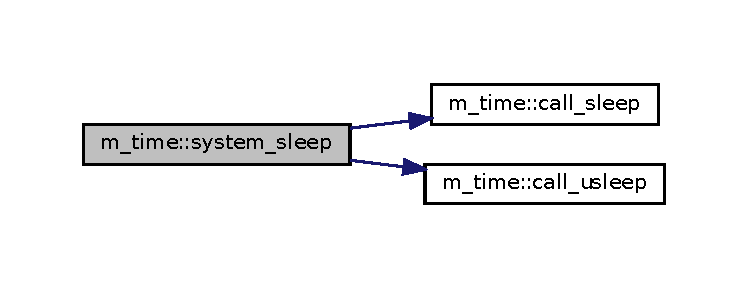
\includegraphics[width=350pt]{namespacem__time_a7c5d028ae1e1e01162ffc7bb55dcbbb1_cgraph}
\end{center}
\end{figure}
\mbox{\Hypertarget{namespacem__time_a083bc231f8ba1879d7f86ab424e77d6c}\label{namespacem__time_a083bc231f8ba1879d7f86ab424e77d6c}} 
\index{m\_time@{m\_time}!u2d@{u2d}}
\index{u2d@{u2d}!m\_time@{m\_time}}
\doxysubsubsection{\texorpdfstring{u2d()}{u2d()}}
{\footnotesize\ttfamily integer function, dimension(8), public m\+\_\+time\+::u2d (\begin{DoxyParamCaption}\item[{class($\ast$), intent(in), optional}]{unixtime }\end{DoxyParamCaption})}

\hypertarget{namespacem__time_autotoc_md184}{}\doxysubsubsection{N\+A\+ME}\label{namespacem__time_autotoc_md184}
u2d(3f) -\/ \mbox{[}M\+\_\+time\+:U\+N\+I\+X\+\_\+\+E\+P\+O\+CH\mbox{]} given Unix Epoch Time returns D\+AT date-\/time array (L\+I\+C\+E\+N\+SE\+:PD)\hypertarget{namespacem__time_autotoc_md185}{}\doxysubsubsection{S\+Y\+N\+O\+P\+S\+IS}\label{namespacem__time_autotoc_md185}
\begin{DoxyVerb}function u2d(unixtime) result (dat)

 class(*),intent(in),optional      :: unixtime
 ! integer
 ! real
 ! real(kind=realtime)

 integer                           :: dat(8)
\end{DoxyVerb}
\hypertarget{namespacem__time_autotoc_md186}{}\doxysubsubsection{D\+E\+S\+C\+R\+I\+P\+T\+I\+ON}\label{namespacem__time_autotoc_md186}
Given Unix Epoch Time returns D\+AT date-\/time array\hypertarget{namespacem__time_autotoc_md187}{}\doxysubsubsection{O\+P\+T\+I\+O\+NS}\label{namespacem__time_autotoc_md187}
unixtime The \char`\"{}\+Unix Epoch\char`\"{} time, or the number of seconds since 00\+:00\+:00 on January 1st, 1970, U\+TC. If not present, use current time.\hypertarget{namespacem__time_autotoc_md188}{}\doxysubsubsection{R\+E\+T\+U\+R\+NS}\label{namespacem__time_autotoc_md188}
dat Integer array holding a \char`\"{}\+D\+A\+T\char`\"{} array, similar in structure to the array returned by the intrinsic D\+A\+T\+E\+\_\+\+A\+N\+D\+\_\+\+T\+I\+M\+E(3f)\+:

dat=\mbox{[} year,month,day,timezone,hour,\& \& minutes,seconds,milliseconds\mbox{]}\hypertarget{namespacem__time_autotoc_md189}{}\doxysubsubsection{E\+X\+A\+M\+P\+LE}\label{namespacem__time_autotoc_md189}
\begin{DoxyVerb}Sample program:

 program demo_u2d
 use M_time, only : u2d, d2u, fmtdate, realtime
 implicit none
 real(kind=realtime) :: today
 integer :: dat(8)
    ! get the date using intrinsic
    call date_and_time(values=dat)
    ! convert today to Julian Date
    today=d2u(dat)
    write(*,*)'Today=',fmtdate(u2d(today))
    ! subtract day
    write(*,*)'Yesterday=',fmtdate(u2d(today-86400.0d0))
    ! add day
    write(*,*)'Tomorrow=',fmtdate(u2d(today+86400.0d0))
 end program demo_u2d

results:

 Today=Tuesday, July 19th, 2016 11:10:08 AM
 Yesterday=Monday, July 18th, 2016 11:10:08 AM
 Tomorrow=Wednesday, July 20th, 2016 11:10:08 AM
\end{DoxyVerb}
\hypertarget{namespacem__time_autotoc_md190}{}\doxysubsubsection{A\+U\+T\+H\+OR}\label{namespacem__time_autotoc_md190}
John S. Urban, 2015 \hypertarget{namespacem__time_autotoc_md191}{}\doxysubsubsection{L\+I\+C\+E\+N\+SE}\label{namespacem__time_autotoc_md191}
Public Domain 

References d2u(), realtime, and unix\+\_\+to\+\_\+date().

Here is the call graph for this function\+:\nopagebreak
\begin{figure}[H]
\begin{center}
\leavevmode
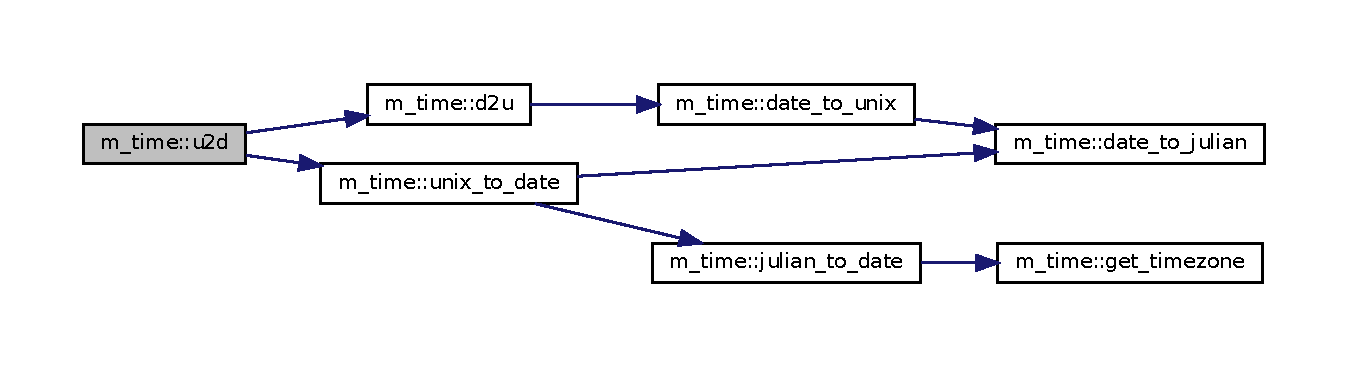
\includegraphics[width=350pt]{namespacem__time_a083bc231f8ba1879d7f86ab424e77d6c_cgraph}
\end{center}
\end{figure}
Here is the caller graph for this function\+:\nopagebreak
\begin{figure}[H]
\begin{center}
\leavevmode
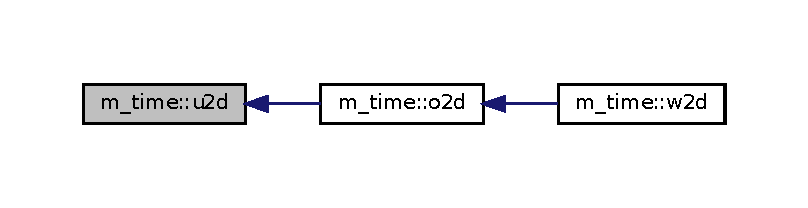
\includegraphics[width=350pt]{namespacem__time_a083bc231f8ba1879d7f86ab424e77d6c_icgraph}
\end{center}
\end{figure}
\mbox{\Hypertarget{namespacem__time_acc62ada23f8fa2fe67b428702fbcbf1c}\label{namespacem__time_acc62ada23f8fa2fe67b428702fbcbf1c}} 
\index{m\_time@{m\_time}!unix\_to\_date@{unix\_to\_date}}
\index{unix\_to\_date@{unix\_to\_date}!m\_time@{m\_time}}
\doxysubsubsection{\texorpdfstring{unix\_to\_date()}{unix\_to\_date()}}
{\footnotesize\ttfamily subroutine, public m\+\_\+time\+::unix\+\_\+to\+\_\+date (\begin{DoxyParamCaption}\item[{class($\ast$), intent(in)}]{unixtime,  }\item[{integer, dimension(8), intent(out)}]{dat,  }\item[{integer, intent(out)}]{ierr }\end{DoxyParamCaption})}

\hypertarget{namespacem__time_autotoc_md26}{}\doxysubsubsection{N\+A\+ME}\label{namespacem__time_autotoc_md26}
unix\+\_\+to\+\_\+date(3f) -\/ \mbox{[}M\+\_\+time\+:U\+N\+I\+X\+\_\+\+E\+P\+O\+CH\mbox{]} converts Unix Epoch Time to D\+AT date-\/time array (L\+I\+C\+E\+N\+SE\+:PD)\hypertarget{namespacem__time_autotoc_md27}{}\doxysubsubsection{S\+Y\+N\+O\+P\+S\+IS}\label{namespacem__time_autotoc_md27}
\begin{DoxyVerb}subroutine unix_to_date(unixtime,dat,ierr)

 real(kind=realtime),intent(in) :: unixtime
 integer,intent(out)            :: dat(8)
 integer,intent(out)            :: ierr
\end{DoxyVerb}
\hypertarget{namespacem__time_autotoc_md28}{}\doxysubsubsection{D\+E\+S\+C\+R\+I\+P\+T\+I\+ON}\label{namespacem__time_autotoc_md28}
Converts a Unix Epoch Time (U\+ET) to a D\+AT date-\/time array.\hypertarget{namespacem__time_autotoc_md29}{}\doxysubsubsection{O\+P\+T\+I\+O\+NS}\label{namespacem__time_autotoc_md29}
\begin{DoxyVerb}unixtime  The "Unix Epoch" time, or the number of seconds since
          00:00:00 on January 1st, 1970, UTC; of type
          real(kind=realtime).
\end{DoxyVerb}
\hypertarget{namespacem__time_autotoc_md30}{}\doxysubsubsection{R\+E\+T\+U\+R\+NS}\label{namespacem__time_autotoc_md30}
dat Integer array holding a \char`\"{}\+D\+A\+T\char`\"{} array, similar in structure to the array returned by the intrinsic D\+A\+T\+E\+\_\+\+A\+N\+D\+\_\+\+T\+I\+M\+E(3f)\+:

dat=\mbox{[} year,month,day,timezone,hour,\& \& minutes,seconds,milliseconds\mbox{]}

ierr Error code. If 0 no error occurred.\hypertarget{namespacem__time_autotoc_md31}{}\doxysubsubsection{E\+X\+A\+M\+P\+LE}\label{namespacem__time_autotoc_md31}
\begin{DoxyVerb} Sample program:

  program demo_unix_to_date
  use M_time, only : unix_to_date, u2d, fmtdate, realtime
  implicit none
  real(kind=realtime)           :: unixtime
  ! seconds in a day
  real(kind=realtime),parameter :: DAY=86400.0d0
  integer                       :: dat(8)
  integer                       :: ierr
     ! sample Unix Epoch time
     unixtime=1468939038.4639933d0
     ! create DAT array for today
     call unix_to_date(unixtime,dat,ierr)
     write(*,*)'Sample Date=',fmtdate(dat)
     ! go back one day
     call unix_to_date(unixtime-DAY,dat,ierr)
     ! subtract day and print
     write(*,*)'Day Before =',fmtdate(dat)
     ! go forward one day
     call unix_to_date(unixtime+DAY,dat,ierr)
     ! add day print
     write(*,*)'Day After  =',fmtdate(dat)
  end program demo_unix_to_date

Results:

 Sample Date=Tuesday, July 19th, 2016 10:37:18 AM
 Day Before =Monday, July 18th, 2016 10:37:18 AM
 Day After  =Wednesday, July 20th, 2016 10:37:18 AM
\end{DoxyVerb}
\hypertarget{namespacem__time_autotoc_md32}{}\doxysubsubsection{A\+U\+T\+H\+OR}\label{namespacem__time_autotoc_md32}
John S. Urban, 2015 \hypertarget{namespacem__time_autotoc_md33}{}\doxysubsubsection{L\+I\+C\+E\+N\+SE}\label{namespacem__time_autotoc_md33}
Public Domain 

References date\+\_\+to\+\_\+julian(), julian\+\_\+to\+\_\+date(), realtime, and secday.

Here is the call graph for this function\+:\nopagebreak
\begin{figure}[H]
\begin{center}
\leavevmode
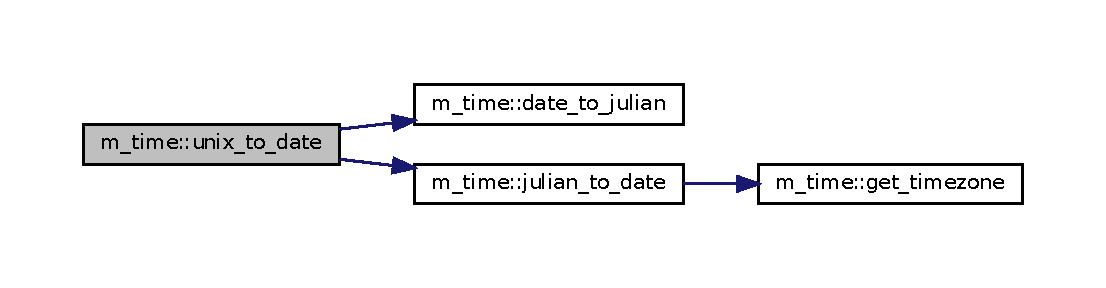
\includegraphics[width=350pt]{namespacem__time_acc62ada23f8fa2fe67b428702fbcbf1c_cgraph}
\end{center}
\end{figure}
Here is the caller graph for this function\+:\nopagebreak
\begin{figure}[H]
\begin{center}
\leavevmode
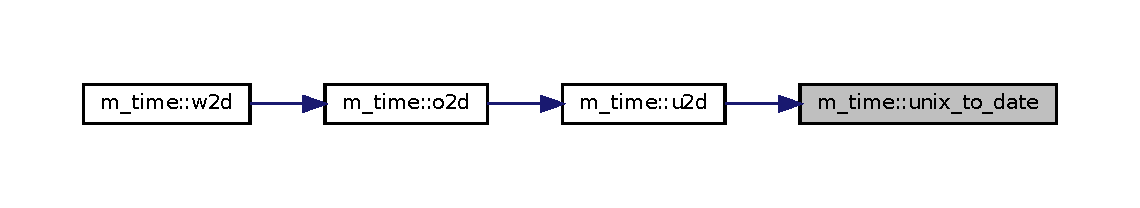
\includegraphics[width=350pt]{namespacem__time_acc62ada23f8fa2fe67b428702fbcbf1c_icgraph}
\end{center}
\end{figure}
\mbox{\Hypertarget{namespacem__time_a6f28cf00e4998bb50bb503f5e4bd3f77}\label{namespacem__time_a6f28cf00e4998bb50bb503f5e4bd3f77}} 
\index{m\_time@{m\_time}!v2mo@{v2mo}}
\index{v2mo@{v2mo}!m\_time@{m\_time}}
\doxysubsubsection{\texorpdfstring{v2mo()}{v2mo()}}
{\footnotesize\ttfamily character(len=\+:) function, allocatable, public m\+\_\+time\+::v2mo (\begin{DoxyParamCaption}\item[{integer, intent(in)}]{imonth }\end{DoxyParamCaption})}

\hypertarget{namespacem__time_autotoc_md62}{}\doxysubsubsection{N\+A\+ME}\label{namespacem__time_autotoc_md62}
v2mo(3f) -\/ \mbox{[}M\+\_\+time\+:M\+O\+N\+T\+H\+\_\+\+N\+A\+ME\mbox{]} returns the month name of a Common month number (L\+I\+C\+E\+N\+SE\+:PD)\hypertarget{namespacem__time_autotoc_md63}{}\doxysubsubsection{S\+Y\+N\+O\+P\+S\+IS}\label{namespacem__time_autotoc_md63}
\begin{DoxyVerb}function v2mo(imonth) result(month_name)

 integer,intent(in)           :: imonth      ! month number (1-12)
 character(len=:),allocatable :: month_name  ! month name
\end{DoxyVerb}
\hypertarget{namespacem__time_autotoc_md64}{}\doxysubsubsection{D\+E\+S\+C\+R\+I\+P\+T\+I\+ON}\label{namespacem__time_autotoc_md64}
Given a Common Calendar month number, return the name of the month as a string.\hypertarget{namespacem__time_autotoc_md65}{}\doxysubsubsection{O\+P\+T\+I\+O\+NS}\label{namespacem__time_autotoc_md65}
imonth Common month number (1-\/12). If out of the allowable range the month name returned will be \textquotesingle{}U\+N\+K\+N\+O\+WN\textquotesingle{}. \hypertarget{namespacem__time_autotoc_md66}{}\doxysubsubsection{R\+E\+T\+U\+R\+NS}\label{namespacem__time_autotoc_md66}
month\+\_\+name A string representing a month name or the word \textquotesingle{}U\+N\+K\+N\+O\+WN\textquotesingle{}\hypertarget{namespacem__time_autotoc_md67}{}\doxysubsubsection{E\+X\+A\+M\+P\+LE}\label{namespacem__time_autotoc_md67}
\begin{DoxyVerb}Sample program:

 program demo_v2mo
 use M_time, only : v2mo
 implicit none
 integer :: i
    write(*,*)(v2mo(i),i=1,13)
 end program demo_v2mo

results:

 January
 February
 March
 April
 May
 June
 July
 August
 September
 October
 November
 December
 UNKNOWN.
\end{DoxyVerb}
 \hypertarget{namespacem__time_autotoc_md68}{}\doxysubsubsection{A\+U\+T\+H\+OR}\label{namespacem__time_autotoc_md68}
John S. Urban, 2015 \hypertarget{namespacem__time_autotoc_md69}{}\doxysubsubsection{L\+I\+C\+E\+N\+SE}\label{namespacem__time_autotoc_md69}
Public Domain Here is the caller graph for this function\+:\nopagebreak
\begin{figure}[H]
\begin{center}
\leavevmode
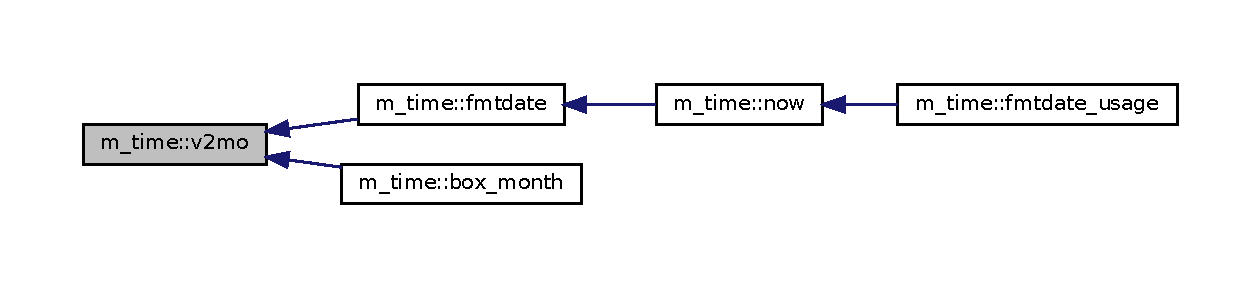
\includegraphics[width=350pt]{namespacem__time_a6f28cf00e4998bb50bb503f5e4bd3f77_icgraph}
\end{center}
\end{figure}
\mbox{\Hypertarget{namespacem__time_ac0ec48db8d508bfa23fe4b20c9d1c5a3}\label{namespacem__time_ac0ec48db8d508bfa23fe4b20c9d1c5a3}} 
\index{m\_time@{m\_time}!w2d@{w2d}}
\index{w2d@{w2d}!m\_time@{m\_time}}
\doxysubsubsection{\texorpdfstring{w2d()}{w2d()}}
{\footnotesize\ttfamily subroutine, public m\+\_\+time\+::w2d (\begin{DoxyParamCaption}\item[{integer, intent(in)}]{iso\+\_\+year,  }\item[{integer, intent(in)}]{iso\+\_\+week,  }\item[{integer, intent(in)}]{iso\+\_\+weekday,  }\item[{integer, dimension(8), intent(out)}]{dat }\end{DoxyParamCaption})}

\hypertarget{namespacem__time_autotoc_md136}{}\doxysubsubsection{N\+A\+ME}\label{namespacem__time_autotoc_md136}
w2d(3f) -\/ \mbox{[}M\+\_\+time\+:W\+E\+E\+K\+\_\+\+O\+F\+\_\+\+Y\+E\+AR\mbox{]} calculate D\+AT date-\/time array from iso-\/8601 Week-\/numbering year date yyyy-\/\+Www-\/d (L\+I\+C\+E\+N\+SE\+:PD)\hypertarget{namespacem__time_autotoc_md137}{}\doxysubsubsection{S\+Y\+N\+O\+P\+S\+IS}\label{namespacem__time_autotoc_md137}
\begin{DoxyVerb}subroutine w2d(iso_year,iso_week,iso_weekday,dat)

 integer,intent(in)      :: iso_year, iso_week, iso_weekday
 integer,intent(out)     :: dat(8)     ! output date array
\end{DoxyVerb}
\hypertarget{namespacem__time_autotoc_md138}{}\doxysubsubsection{D\+E\+S\+C\+R\+I\+P\+T\+I\+ON}\label{namespacem__time_autotoc_md138}
Given an I\+S\+O-\/8601 week return a \char`\"{}\+D\+A\+T\char`\"{} array defining a date and time, The I\+S\+O-\/8601 is supplied as three integer values defining the I\+SO year, week of year and weekday.\hypertarget{namespacem__time_autotoc_md139}{}\doxysubsubsection{O\+P\+T\+I\+O\+NS}\label{namespacem__time_autotoc_md139}
iso\+\_\+year I\+S\+O-\/8601 year number for the given date iso\+\_\+week I\+S\+O-\/8601 week number for the given date iso\+\_\+weekday I\+S\+O-\/8601 weekday number for the given date iso\+\_\+name I\+S\+O-\/8601 Week string for the data in the form \char`\"{}yyyy-\/\+Www-\/d\char`\"{}.\hypertarget{namespacem__time_autotoc_md140}{}\doxysubsubsection{R\+E\+T\+U\+R\+NS}\label{namespacem__time_autotoc_md140}
dat \char`\"{}\+D\+A\+T\char`\"{} array (an integer array of the same format as the array returned by the intrinsic D\+A\+T\+E\+\_\+\+A\+N\+D\+\_\+\+T\+I\+M\+E(3f)) describing the date to be used, which is the basic time description used by the other M\+\_\+time(3fm) module procedures.\hypertarget{namespacem__time_autotoc_md141}{}\doxysubsubsection{E\+X\+A\+M\+P\+LE}\label{namespacem__time_autotoc_md141}
Sample program\+:

program demo\+\_\+w2d use M\+\_\+time, only \+: w2d, fmtdate implicit none write($\ast$,\textquotesingle{}(a)\textquotesingle{})\& \& \textquotesingle{}Given Monday 29 December 2008 is written \char`\"{}2009-\/\+W01-\/1\char`\"{}\textquotesingle{} call printit(2009,1,1) write($\ast$,\textquotesingle{}(a)\textquotesingle{})\& \& \textquotesingle{}Given Sunday 3 January 2010 is written \char`\"{}2009-\/\+W53-\/7\char`\"{}\textquotesingle{} call printit(2009,53,7) write($\ast$,\textquotesingle{}(a)\textquotesingle{})\& \& \textquotesingle{}Given the Gregorian date Sun 31 December 2006 \& \&is written 2006-\/W52-\/7\textquotesingle{} call printit(2006,52,7) write($\ast$,\textquotesingle{}(a)\textquotesingle{})\& \& \textquotesingle{}Given 27 September 2008 is 2008-\/W39-\/6\textquotesingle{} call printit(2008,39,6) contains subroutine printit(iso\+\_\+year,iso\+\_\+week,iso\+\_\+weekday) ! I\+S\+O-\/8601 Week\+: 2016-\/W29-\/1 integer \+:: iso\+\_\+year, iso\+\_\+week, iso\+\_\+weekday ! input date array integer \+:: dat(8) call w2d(iso\+\_\+year,iso\+\_\+week,iso\+\_\+weekday,dat) write($\ast$,\textquotesingle{}(a,i0)\textquotesingle{})\textquotesingle{}G\+I\+V\+EN\+: \textquotesingle{} write($\ast$,\textquotesingle{}(a,i0)\textquotesingle{})\textquotesingle{}I\+S\+O-\/8601 year \textquotesingle{},iso\+\_\+year write($\ast$,\textquotesingle{}(a,i0)\textquotesingle{})\textquotesingle{}I\+S\+O-\/8601 week \textquotesingle{},iso\+\_\+week write($\ast$,\textquotesingle{}(a,i0)\textquotesingle{})\textquotesingle{}I\+S\+O-\/8601 weekday \textquotesingle{},iso\+\_\+weekday write($\ast$,\textquotesingle{}(a,i0)\textquotesingle{})\textquotesingle{}R\+E\+S\+U\+LT\+: \textquotesingle{} write($\ast$,\textquotesingle{}(a,$\ast$(i0\+:,\char`\"{},\char`\"{}))\textquotesingle{})\textquotesingle{} D\+AT array \textquotesingle{},dat write($\ast$,\textquotesingle{}(a,/,67(\char`\"{}=\char`\"{}))\textquotesingle{})\textquotesingle{} \textquotesingle{}//fmtdate(dat,\textquotesingle{}long\textquotesingle{}) end subroutine printit end program demo\+\_\+w2d

Results\+:

Given Monday 29 December 2008 is written \char`\"{}2009-\/\+W01-\/1\char`\"{} G\+I\+V\+EN\+: I\+S\+O-\/8601 year 2009 I\+S\+O-\/8601 week 1 I\+S\+O-\/8601 weekday 1 R\+E\+S\+U\+LT\+: D\+AT array 2008,12,29,-\/240,0,0,0,0 \hypertarget{namespacem__time_autotoc_md142}{}\doxysubsection{Monday, December 29th, 2008 12\+:00\+:00 A\+M U\+T\+C-\/04\+:00}\label{namespacem__time_autotoc_md142}
Given Sunday 3 January 2010 is written \char`\"{}2009-\/\+W53-\/7\char`\"{} G\+I\+V\+EN\+: I\+S\+O-\/8601 year 2009 I\+S\+O-\/8601 week 53 I\+S\+O-\/8601 weekday 7 R\+E\+S\+U\+LT\+: D\+AT array 2010,1,3,-\/240,0,0,0,0 \hypertarget{namespacem__time_autotoc_md143}{}\doxysubsection{Sunday, January 3rd, 2010 12\+:00\+:00 A\+M U\+T\+C-\/04\+:00}\label{namespacem__time_autotoc_md143}
Given the Gregorian date Sun 31 December 2006 is written 2006-\/W52-\/7 G\+I\+V\+EN\+: I\+S\+O-\/8601 year 2006 I\+S\+O-\/8601 week 52 I\+S\+O-\/8601 weekday 7 R\+E\+S\+U\+LT\+: D\+AT array 2006,12,31,-\/240,0,0,0,0 \hypertarget{namespacem__time_autotoc_md144}{}\doxysubsection{Sunday, December 31st, 2006 12\+:00\+:00 A\+M U\+T\+C-\/04\+:00}\label{namespacem__time_autotoc_md144}
Given 27 September 2008 is 2008-\/W39-\/6 G\+I\+V\+EN\+: I\+S\+O-\/8601 year 2008 I\+S\+O-\/8601 week 39 I\+S\+O-\/8601 weekday 6 R\+E\+S\+U\+LT\+: D\+AT array 2008,9,27,-\/240,0,0,0,0 \hypertarget{namespacem__time_autotoc_md145}{}\doxysubsection{Saturday, September 27th, 2008 12\+:00\+:00 A\+M U\+T\+C-\/04\+:00}\label{namespacem__time_autotoc_md145}
\hypertarget{namespacem__time_autotoc_md146}{}\doxysubsubsection{D\+E\+F\+I\+N\+I\+T\+I\+ON}\label{namespacem__time_autotoc_md146}
The I\+S\+O-\/8601 date and time standard was issued by the International Organization for Standardization (I\+SO). It is used (mainly) in government and business for fiscal years, as well as in timekeeping. The system specifies a week year atop the Gregorian calendar by defining a notation for ordinal weeks of the year.

An I\+SO week-\/numbering year (also called I\+SO year informally) has 52 or 53 full weeks. That is 364 or 371 days instead of the usual 365 or 366 days. The extra week is referred to here as a leap week, although I\+S\+O-\/8601 does not use this term. Weeks start with Monday. The first week of a year is the week that contains the first Thursday of the year (and, hence, always contains 4 January). I\+SO week year numbering therefore slightly deviates from the Gregorian for some days close to January 1st.\hypertarget{namespacem__time_autotoc_md147}{}\doxysubsubsection{M\+E\+T\+H\+OD}\label{namespacem__time_autotoc_md147}
Calculating a date given the year, week number and weekday

This method requires that one know the weekday of 4 January of the year in question. Add 3 to the number of this weekday, giving a correction to be used for dates within this year.

Method\+: Multiply the week number by 7, then add the weekday. From this sum subtract the correction for the year. The result is the ordinal date, which can be converted into a calendar date. If the ordinal date thus obtained is zero or negative, the date belongs to the previous calendar year; if greater than the number of days in the year, to the following year.

Example\+: year 2008, week 39, Saturday (day 6) Correction for 2008\+: 5 + 3 = 8 (39 x 7) + 6 = 279 279 -\/ 8 = 271 Ordinal day 271 of a leap year is day 271 -\/ 244 = 27 September Result\+: 27 September 2008\hypertarget{namespacem__time_autotoc_md148}{}\doxysubsubsection{I\+S\+O\+\_\+\+N\+A\+ME}\label{namespacem__time_autotoc_md148}
Week date representations are in the format Y\+Y\+Y\+Y\+Www-\/D.

o \mbox{[}Y\+Y\+YY\mbox{]} indicates the I\+SO week-\/numbering year which is slightly different from the traditional Gregorian calendar year. o \mbox{[}Www\mbox{]} is the week number prefixed by the letter W, from W01 through W53. o \mbox{[}D\mbox{]} is the weekday number, from 1 through 7, beginning with Monday and ending with Sunday.

For example, the Gregorian date 31 December 2006 corresponds to the Sunday of the 52nd week of 2006, and is written

2006-\/W52-\/7 (extended form) or 2006W527 (compact form).\hypertarget{namespacem__time_autotoc_md149}{}\doxysubsubsection{R\+E\+F\+E\+R\+E\+N\+CE}\label{namespacem__time_autotoc_md149}
From Wikipedia, the free encyclopedia 2016-\/08-\/08\hypertarget{namespacem__time_autotoc_md150}{}\doxysubsubsection{A\+U\+T\+H\+OR}\label{namespacem__time_autotoc_md150}
John S. Urban, 2015 \hypertarget{namespacem__time_autotoc_md151}{}\doxysubsubsection{L\+I\+C\+E\+N\+SE}\label{namespacem__time_autotoc_md151}
Public Domain 

References dow(), and o2d().

Here is the call graph for this function\+:\nopagebreak
\begin{figure}[H]
\begin{center}
\leavevmode
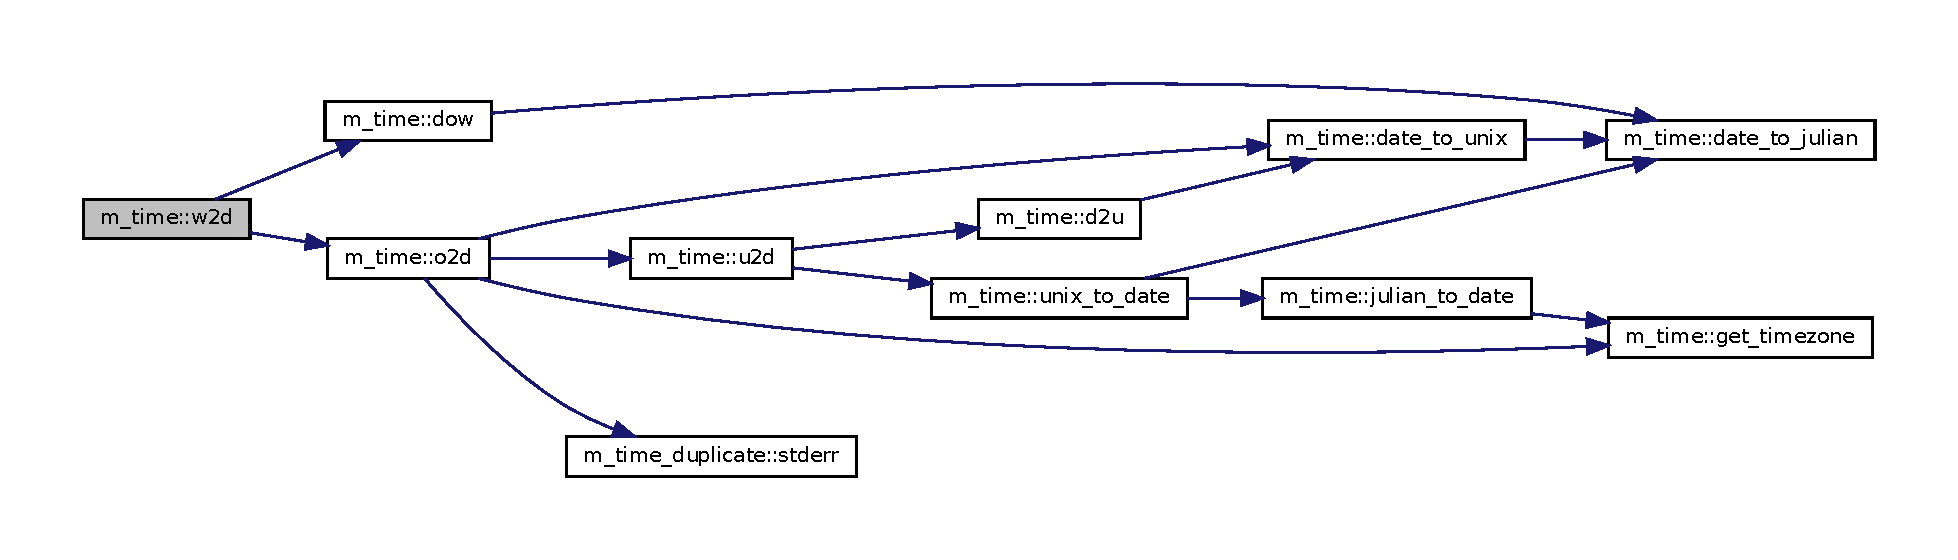
\includegraphics[width=350pt]{namespacem__time_ac0ec48db8d508bfa23fe4b20c9d1c5a3_cgraph}
\end{center}
\end{figure}


\doxysubsection{Variable Documentation}
\mbox{\Hypertarget{namespacem__time_a97725f8d657c24badff19a794f323a6b}\label{namespacem__time_a97725f8d657c24badff19a794f323a6b}} 
\index{m\_time@{m\_time}!dt\_day@{dt\_day}}
\index{dt\_day@{dt\_day}!m\_time@{m\_time}}
\doxysubsubsection{\texorpdfstring{dt\_day}{dt\_day}}
{\footnotesize\ttfamily real(kind=\mbox{\hyperlink{namespacem__time_ac10ea9e8d59ec74eaa7d89f2517d7422}{realtime}}), parameter, public m\+\_\+time\+::dt\+\_\+day =86400.\+0d0}

\mbox{\Hypertarget{namespacem__time_aa0ca2172092f5e7dcc9b8524e6516fd8}\label{namespacem__time_aa0ca2172092f5e7dcc9b8524e6516fd8}} 
\index{m\_time@{m\_time}!dt\_hour@{dt\_hour}}
\index{dt\_hour@{dt\_hour}!m\_time@{m\_time}}
\doxysubsubsection{\texorpdfstring{dt\_hour}{dt\_hour}}
{\footnotesize\ttfamily real(kind=\mbox{\hyperlink{namespacem__time_ac10ea9e8d59ec74eaa7d89f2517d7422}{realtime}}), parameter, public m\+\_\+time\+::dt\+\_\+hour =3600.\+0d0}

\mbox{\Hypertarget{namespacem__time_a9fe6fbb44e2779a2fcf96fba36c08918}\label{namespacem__time_a9fe6fbb44e2779a2fcf96fba36c08918}} 
\index{m\_time@{m\_time}!dt\_minute@{dt\_minute}}
\index{dt\_minute@{dt\_minute}!m\_time@{m\_time}}
\doxysubsubsection{\texorpdfstring{dt\_minute}{dt\_minute}}
{\footnotesize\ttfamily real(kind=\mbox{\hyperlink{namespacem__time_ac10ea9e8d59ec74eaa7d89f2517d7422}{realtime}}), parameter, public m\+\_\+time\+::dt\+\_\+minute =60.\+0d0}

\mbox{\Hypertarget{namespacem__time_a3d53519e90264faccdae67e389ffc003}\label{namespacem__time_a3d53519e90264faccdae67e389ffc003}} 
\index{m\_time@{m\_time}!dt\_week@{dt\_week}}
\index{dt\_week@{dt\_week}!m\_time@{m\_time}}
\doxysubsubsection{\texorpdfstring{dt\_week}{dt\_week}}
{\footnotesize\ttfamily real(kind=\mbox{\hyperlink{namespacem__time_ac10ea9e8d59ec74eaa7d89f2517d7422}{realtime}}), parameter, public m\+\_\+time\+::dt\+\_\+week =\mbox{\hyperlink{namespacem__time_a97725f8d657c24badff19a794f323a6b}{dt\+\_\+day}}$\ast$7.\+0d0}

\mbox{\Hypertarget{namespacem__time_ac10ea9e8d59ec74eaa7d89f2517d7422}\label{namespacem__time_ac10ea9e8d59ec74eaa7d89f2517d7422}} 
\index{m\_time@{m\_time}!realtime@{realtime}}
\index{realtime@{realtime}!m\_time@{m\_time}}
\doxysubsubsection{\texorpdfstring{realtime}{realtime}}
{\footnotesize\ttfamily integer, parameter, public m\+\_\+time\+::realtime =kind(0.\+0d0)}

\mbox{\Hypertarget{namespacem__time_a48130b5a95a3f2e776269dcee1426797}\label{namespacem__time_a48130b5a95a3f2e776269dcee1426797}} 
\index{m\_time@{m\_time}!secday@{secday}}
\index{secday@{secday}!m\_time@{m\_time}}
\doxysubsubsection{\texorpdfstring{secday}{secday}}
{\footnotesize\ttfamily real(kind=\mbox{\hyperlink{namespacem__time_ac10ea9e8d59ec74eaa7d89f2517d7422}{realtime}}), parameter, private m\+\_\+time\+::secday =86400.\+0d0\hspace{0.3cm}{\ttfamily [private]}}


\chapter{Data Type Documentation}
\hypertarget{structm__time_1_1date__time}{}\section{m\+\_\+time\+:\+:date\+\_\+time Interface Reference}
\label{structm__time_1_1date__time}\index{m\+\_\+time\+::date\+\_\+time@{m\+\_\+time\+::date\+\_\+time}}
\subsection*{Private Member Functions}
\begin{DoxyCompactItemize}
\item 
procedure \mbox{\hyperlink{structm__time_1_1date__time_a69ded91df8430fd8bacc28c8206dbba1}{datout}} =$>$ \mbox{\hyperlink{namespacem__time_aa281690d7f68f14842b00d238702e774}{dt2d}}
\item 
procedure \mbox{\hyperlink{structm__time_1_1date__time_a82e907454834f91e7aa081755367f81b}{epoch}}
\item 
procedure \mbox{\hyperlink{structm__time_1_1date__time_a213c4d0b61c448585796955c2e336dcc}{julian}} =$>$ \mbox{\hyperlink{namespacem__time_aff0a1b524b578e85efe20b87fbe9db61}{julian\+\_\+oop}}
\item 
procedure \mbox{\hyperlink{structm__time_1_1date__time_a0020bfaff4b78b7b0688dada7997d9f6}{ordinal}} =$>$ \mbox{\hyperlink{namespacem__time_a7fb507bb72a1872ec2a86fb7f3a50d75}{ordinal\+\_\+oop}}
\item 
procedure \mbox{\hyperlink{structm__time_1_1date__time_abfb29551ce7b06e12ae947bac78cd345}{weekday}} =$>$ \mbox{\hyperlink{namespacem__time_ac43e082c8ffd7687c4fc91beddc15720}{weekday\+\_\+oop}}
\item 
procedure \mbox{\hyperlink{structm__time_1_1date__time_acb5b22e87e6cf552a3d309bb0ead2275}{format}}
\item 
procedure \mbox{\hyperlink{structm__time_1_1date__time_aed911f77f6ec0b0572a0ea5ab03351df}{delta}}
\item 
procedure \mbox{\hyperlink{structm__time_1_1date__time_aac1087f981460b9eae1aa73e17c9943c}{init}} =$>$ \mbox{\hyperlink{namespacem__time_a72455f763954fae8ebc0f454033d82a8}{init\+\_\+dt}}
\item 
procedure, private \mbox{\hyperlink{structm__time_1_1date__time_a05e1950f16d81be0499b403b7e369b40}{plus\+\_\+seconds}}
\item 
generic \mbox{\hyperlink{structm__time_1_1date__time_ad51508db1d161547062f40dcd91f4e4b}{operator}} =$>$ \mbox{\hyperlink{structm__time_1_1date__time_a05e1950f16d81be0499b403b7e369b40}{plus\+\_\+seconds}}
\item 
procedure, private \mbox{\hyperlink{structm__time_1_1date__time_ac1002f3185c442747e93479fe136c725}{eq}}
\item 
generic \mbox{\hyperlink{structm__time_1_1date__time_a67028b37f0375d0209cb6379c59d99e5}{operator}} =$>$ \mbox{\hyperlink{structm__time_1_1date__time_ac1002f3185c442747e93479fe136c725}{eq}}
\item 
procedure, private \mbox{\hyperlink{structm__time_1_1date__time_aa4f036a923d45e10e6f6251945b375ad}{lt}}
\item 
generic \mbox{\hyperlink{structm__time_1_1date__time_afd5a2b9837bc8d48eb244bd07c200c6a}{operator}} =$>$ \mbox{\hyperlink{structm__time_1_1date__time_aa4f036a923d45e10e6f6251945b375ad}{lt}}
\item 
procedure, private \mbox{\hyperlink{structm__time_1_1date__time_aadb4377349cd5d9b003b1287d276dddf}{gt}}
\item 
generic \mbox{\hyperlink{structm__time_1_1date__time_a1aa01f75ae1f67a4b3202febd56b462f}{operator}} =$>$ \mbox{\hyperlink{structm__time_1_1date__time_aadb4377349cd5d9b003b1287d276dddf}{gt}}
\item 
procedure, private \mbox{\hyperlink{structm__time_1_1date__time_ac81a50f7827211f12a738e1acc278f51}{ge}}
\item 
generic \mbox{\hyperlink{structm__time_1_1date__time_a3961b17820108c6eb0037d11a03cfcd2}{operator}} =$>$ \mbox{\hyperlink{structm__time_1_1date__time_ac81a50f7827211f12a738e1acc278f51}{ge}}
\item 
procedure, private \mbox{\hyperlink{structm__time_1_1date__time_a3733467846b084981cf74e4f3d615c13}{le}}
\item 
generic \mbox{\hyperlink{structm__time_1_1date__time_add9b1c423294accdf967e22fa61a7796}{operator}} =$>$ \mbox{\hyperlink{structm__time_1_1date__time_a3733467846b084981cf74e4f3d615c13}{le}}
\item 
procedure, private \mbox{\hyperlink{structm__time_1_1date__time_a4d9e08f2f8d3c8a9f3442297900891ec}{ne}}
\item 
generic \mbox{\hyperlink{structm__time_1_1date__time_af93a94ed420ca7ba08cc63c36e88459c}{operator}} =$>$ \mbox{\hyperlink{structm__time_1_1date__time_a4d9e08f2f8d3c8a9f3442297900891ec}{ne}}
\item 
procedure, private \mbox{\hyperlink{structm__time_1_1date__time_a54751a9b71d326e9ff2398031fcf0de9}{minus\+\_\+seconds}}
\item 
procedure, private \mbox{\hyperlink{structm__time_1_1date__time_a590025bad9fe71932ef3d06ca4a3c613}{minus\+\_\+date\+\_\+time}}
\item 
generic \mbox{\hyperlink{structm__time_1_1date__time_affafbae65afa1e12c901241e641e4b1f}{operator}} =$>$ \mbox{\hyperlink{structm__time_1_1date__time_a54751a9b71d326e9ff2398031fcf0de9}{minus\+\_\+seconds}}
\item 
generic \mbox{\hyperlink{structm__time_1_1date__time_adc11c2984fd9dae163e44627a5e2a134}{operator}} =$>$ \mbox{\hyperlink{structm__time_1_1date__time_a590025bad9fe71932ef3d06ca4a3c613}{minus\+\_\+date\+\_\+time}}
\item 
type(\mbox{\hyperlink{structm__time_1_1date__time}{date\+\_\+time}}) function \mbox{\hyperlink{structm__time_1_1date__time_aa431f7c4e9a44ca1ddb3446b28f53547}{construct\+\_\+from\+\_\+dat}} (dat)
\end{DoxyCompactItemize}
\subsection*{Private Attributes}
\begin{DoxyCompactItemize}
\item 
integer \mbox{\hyperlink{structm__time_1_1date__time_aadd87661407a53f0b50fe7fc47038f52}{year}} =1970
\item 
integer \mbox{\hyperlink{structm__time_1_1date__time_aa0360a36979a7e0f621770379d432032}{month}} =1
\item 
integer \mbox{\hyperlink{structm__time_1_1date__time_a7bfa953907e96e82128a4ab5eac0a33e}{day}} =1
\item 
integer \mbox{\hyperlink{structm__time_1_1date__time_a74edfe999538728025d729a7ce69fddc}{tz}} =0
\item 
integer \mbox{\hyperlink{structm__time_1_1date__time_a95fab5ef1aea89d18411f26f34192f1a}{hour}} =0
\item 
integer \mbox{\hyperlink{structm__time_1_1date__time_a9ac3edac50f8a4aae577b1c889404837}{minute}} =0
\item 
integer \mbox{\hyperlink{structm__time_1_1date__time_a22161ace4be90b741a1600435588fc64}{second}} =0
\item 
integer \mbox{\hyperlink{structm__time_1_1date__time_a9a2f1be9348dd330a30ffd207c0791fc}{millisecond}} =0
\end{DoxyCompactItemize}


\subsection{Member Function/\+Subroutine Documentation}
\mbox{\Hypertarget{structm__time_1_1date__time_aa431f7c4e9a44ca1ddb3446b28f53547}\label{structm__time_1_1date__time_aa431f7c4e9a44ca1ddb3446b28f53547}} 
\index{m\+\_\+time\+::date\+\_\+time@{m\+\_\+time\+::date\+\_\+time}!construct\+\_\+from\+\_\+dat@{construct\+\_\+from\+\_\+dat}}
\index{construct\+\_\+from\+\_\+dat@{construct\+\_\+from\+\_\+dat}!m\+\_\+time\+::date\+\_\+time@{m\+\_\+time\+::date\+\_\+time}}
\subsubsection{\texorpdfstring{construct\+\_\+from\+\_\+dat()}{construct\_from\_dat()}}
{\footnotesize\ttfamily type(\mbox{\hyperlink{structm__time_1_1date__time}{date\+\_\+time}}) function m\+\_\+time\+::date\+\_\+time\+::construct\+\_\+from\+\_\+dat (\begin{DoxyParamCaption}\item[{integer, dimension(\+:), intent(in)}]{dat }\end{DoxyParamCaption})\hspace{0.3cm}{\ttfamily [private]}}

\mbox{\Hypertarget{structm__time_1_1date__time_a69ded91df8430fd8bacc28c8206dbba1}\label{structm__time_1_1date__time_a69ded91df8430fd8bacc28c8206dbba1}} 
\index{m\+\_\+time\+::date\+\_\+time@{m\+\_\+time\+::date\+\_\+time}!datout@{datout}}
\index{datout@{datout}!m\+\_\+time\+::date\+\_\+time@{m\+\_\+time\+::date\+\_\+time}}
\subsubsection{\texorpdfstring{datout()}{datout()}}
{\footnotesize\ttfamily procedure m\+\_\+time\+::date\+\_\+time\+::datout (\begin{DoxyParamCaption}{ }\end{DoxyParamCaption})\hspace{0.3cm}{\ttfamily [private]}}

\mbox{\Hypertarget{structm__time_1_1date__time_aed911f77f6ec0b0572a0ea5ab03351df}\label{structm__time_1_1date__time_aed911f77f6ec0b0572a0ea5ab03351df}} 
\index{m\+\_\+time\+::date\+\_\+time@{m\+\_\+time\+::date\+\_\+time}!delta@{delta}}
\index{delta@{delta}!m\+\_\+time\+::date\+\_\+time@{m\+\_\+time\+::date\+\_\+time}}
\subsubsection{\texorpdfstring{delta()}{delta()}}
{\footnotesize\ttfamily procedure m\+\_\+time\+::date\+\_\+time\+::delta (\begin{DoxyParamCaption}{ }\end{DoxyParamCaption})\hspace{0.3cm}{\ttfamily [private]}}

\mbox{\Hypertarget{structm__time_1_1date__time_a82e907454834f91e7aa081755367f81b}\label{structm__time_1_1date__time_a82e907454834f91e7aa081755367f81b}} 
\index{m\+\_\+time\+::date\+\_\+time@{m\+\_\+time\+::date\+\_\+time}!epoch@{epoch}}
\index{epoch@{epoch}!m\+\_\+time\+::date\+\_\+time@{m\+\_\+time\+::date\+\_\+time}}
\subsubsection{\texorpdfstring{epoch()}{epoch()}}
{\footnotesize\ttfamily procedure m\+\_\+time\+::date\+\_\+time\+::epoch (\begin{DoxyParamCaption}{ }\end{DoxyParamCaption})\hspace{0.3cm}{\ttfamily [private]}}

\mbox{\Hypertarget{structm__time_1_1date__time_ac1002f3185c442747e93479fe136c725}\label{structm__time_1_1date__time_ac1002f3185c442747e93479fe136c725}} 
\index{m\+\_\+time\+::date\+\_\+time@{m\+\_\+time\+::date\+\_\+time}!eq@{eq}}
\index{eq@{eq}!m\+\_\+time\+::date\+\_\+time@{m\+\_\+time\+::date\+\_\+time}}
\subsubsection{\texorpdfstring{eq()}{eq()}}
{\footnotesize\ttfamily procedure, private m\+\_\+time\+::date\+\_\+time\+::eq (\begin{DoxyParamCaption}{ }\end{DoxyParamCaption})\hspace{0.3cm}{\ttfamily [private]}}

\mbox{\Hypertarget{structm__time_1_1date__time_acb5b22e87e6cf552a3d309bb0ead2275}\label{structm__time_1_1date__time_acb5b22e87e6cf552a3d309bb0ead2275}} 
\index{m\+\_\+time\+::date\+\_\+time@{m\+\_\+time\+::date\+\_\+time}!format@{format}}
\index{format@{format}!m\+\_\+time\+::date\+\_\+time@{m\+\_\+time\+::date\+\_\+time}}
\subsubsection{\texorpdfstring{format()}{format()}}
{\footnotesize\ttfamily procedure m\+\_\+time\+::date\+\_\+time\+::format (\begin{DoxyParamCaption}{ }\end{DoxyParamCaption})\hspace{0.3cm}{\ttfamily [private]}}

\mbox{\Hypertarget{structm__time_1_1date__time_ac81a50f7827211f12a738e1acc278f51}\label{structm__time_1_1date__time_ac81a50f7827211f12a738e1acc278f51}} 
\index{m\+\_\+time\+::date\+\_\+time@{m\+\_\+time\+::date\+\_\+time}!ge@{ge}}
\index{ge@{ge}!m\+\_\+time\+::date\+\_\+time@{m\+\_\+time\+::date\+\_\+time}}
\subsubsection{\texorpdfstring{ge()}{ge()}}
{\footnotesize\ttfamily procedure, private m\+\_\+time\+::date\+\_\+time\+::ge (\begin{DoxyParamCaption}{ }\end{DoxyParamCaption})\hspace{0.3cm}{\ttfamily [private]}}

\mbox{\Hypertarget{structm__time_1_1date__time_aadb4377349cd5d9b003b1287d276dddf}\label{structm__time_1_1date__time_aadb4377349cd5d9b003b1287d276dddf}} 
\index{m\+\_\+time\+::date\+\_\+time@{m\+\_\+time\+::date\+\_\+time}!gt@{gt}}
\index{gt@{gt}!m\+\_\+time\+::date\+\_\+time@{m\+\_\+time\+::date\+\_\+time}}
\subsubsection{\texorpdfstring{gt()}{gt()}}
{\footnotesize\ttfamily procedure, private m\+\_\+time\+::date\+\_\+time\+::gt (\begin{DoxyParamCaption}{ }\end{DoxyParamCaption})\hspace{0.3cm}{\ttfamily [private]}}

\mbox{\Hypertarget{structm__time_1_1date__time_aac1087f981460b9eae1aa73e17c9943c}\label{structm__time_1_1date__time_aac1087f981460b9eae1aa73e17c9943c}} 
\index{m\+\_\+time\+::date\+\_\+time@{m\+\_\+time\+::date\+\_\+time}!init@{init}}
\index{init@{init}!m\+\_\+time\+::date\+\_\+time@{m\+\_\+time\+::date\+\_\+time}}
\subsubsection{\texorpdfstring{init()}{init()}}
{\footnotesize\ttfamily procedure m\+\_\+time\+::date\+\_\+time\+::init (\begin{DoxyParamCaption}{ }\end{DoxyParamCaption})\hspace{0.3cm}{\ttfamily [private]}}

\mbox{\Hypertarget{structm__time_1_1date__time_a213c4d0b61c448585796955c2e336dcc}\label{structm__time_1_1date__time_a213c4d0b61c448585796955c2e336dcc}} 
\index{m\+\_\+time\+::date\+\_\+time@{m\+\_\+time\+::date\+\_\+time}!julian@{julian}}
\index{julian@{julian}!m\+\_\+time\+::date\+\_\+time@{m\+\_\+time\+::date\+\_\+time}}
\subsubsection{\texorpdfstring{julian()}{julian()}}
{\footnotesize\ttfamily procedure m\+\_\+time\+::date\+\_\+time\+::julian (\begin{DoxyParamCaption}{ }\end{DoxyParamCaption})\hspace{0.3cm}{\ttfamily [private]}}

\mbox{\Hypertarget{structm__time_1_1date__time_a3733467846b084981cf74e4f3d615c13}\label{structm__time_1_1date__time_a3733467846b084981cf74e4f3d615c13}} 
\index{m\+\_\+time\+::date\+\_\+time@{m\+\_\+time\+::date\+\_\+time}!le@{le}}
\index{le@{le}!m\+\_\+time\+::date\+\_\+time@{m\+\_\+time\+::date\+\_\+time}}
\subsubsection{\texorpdfstring{le()}{le()}}
{\footnotesize\ttfamily procedure, private m\+\_\+time\+::date\+\_\+time\+::le (\begin{DoxyParamCaption}{ }\end{DoxyParamCaption})\hspace{0.3cm}{\ttfamily [private]}}

\mbox{\Hypertarget{structm__time_1_1date__time_aa4f036a923d45e10e6f6251945b375ad}\label{structm__time_1_1date__time_aa4f036a923d45e10e6f6251945b375ad}} 
\index{m\+\_\+time\+::date\+\_\+time@{m\+\_\+time\+::date\+\_\+time}!lt@{lt}}
\index{lt@{lt}!m\+\_\+time\+::date\+\_\+time@{m\+\_\+time\+::date\+\_\+time}}
\subsubsection{\texorpdfstring{lt()}{lt()}}
{\footnotesize\ttfamily procedure, private m\+\_\+time\+::date\+\_\+time\+::lt (\begin{DoxyParamCaption}{ }\end{DoxyParamCaption})\hspace{0.3cm}{\ttfamily [private]}}

\mbox{\Hypertarget{structm__time_1_1date__time_a590025bad9fe71932ef3d06ca4a3c613}\label{structm__time_1_1date__time_a590025bad9fe71932ef3d06ca4a3c613}} 
\index{m\+\_\+time\+::date\+\_\+time@{m\+\_\+time\+::date\+\_\+time}!minus\+\_\+date\+\_\+time@{minus\+\_\+date\+\_\+time}}
\index{minus\+\_\+date\+\_\+time@{minus\+\_\+date\+\_\+time}!m\+\_\+time\+::date\+\_\+time@{m\+\_\+time\+::date\+\_\+time}}
\subsubsection{\texorpdfstring{minus\+\_\+date\+\_\+time()}{minus\_date\_time()}}
{\footnotesize\ttfamily procedure, private m\+\_\+time\+::date\+\_\+time\+::minus\+\_\+date\+\_\+time (\begin{DoxyParamCaption}{ }\end{DoxyParamCaption})\hspace{0.3cm}{\ttfamily [private]}}

\mbox{\Hypertarget{structm__time_1_1date__time_a54751a9b71d326e9ff2398031fcf0de9}\label{structm__time_1_1date__time_a54751a9b71d326e9ff2398031fcf0de9}} 
\index{m\+\_\+time\+::date\+\_\+time@{m\+\_\+time\+::date\+\_\+time}!minus\+\_\+seconds@{minus\+\_\+seconds}}
\index{minus\+\_\+seconds@{minus\+\_\+seconds}!m\+\_\+time\+::date\+\_\+time@{m\+\_\+time\+::date\+\_\+time}}
\subsubsection{\texorpdfstring{minus\+\_\+seconds()}{minus\_seconds()}}
{\footnotesize\ttfamily procedure, private m\+\_\+time\+::date\+\_\+time\+::minus\+\_\+seconds (\begin{DoxyParamCaption}{ }\end{DoxyParamCaption})\hspace{0.3cm}{\ttfamily [private]}}

\mbox{\Hypertarget{structm__time_1_1date__time_a4d9e08f2f8d3c8a9f3442297900891ec}\label{structm__time_1_1date__time_a4d9e08f2f8d3c8a9f3442297900891ec}} 
\index{m\+\_\+time\+::date\+\_\+time@{m\+\_\+time\+::date\+\_\+time}!ne@{ne}}
\index{ne@{ne}!m\+\_\+time\+::date\+\_\+time@{m\+\_\+time\+::date\+\_\+time}}
\subsubsection{\texorpdfstring{ne()}{ne()}}
{\footnotesize\ttfamily procedure, private m\+\_\+time\+::date\+\_\+time\+::ne (\begin{DoxyParamCaption}{ }\end{DoxyParamCaption})\hspace{0.3cm}{\ttfamily [private]}}

\mbox{\Hypertarget{structm__time_1_1date__time_ad51508db1d161547062f40dcd91f4e4b}\label{structm__time_1_1date__time_ad51508db1d161547062f40dcd91f4e4b}} 
\index{m\+\_\+time\+::date\+\_\+time@{m\+\_\+time\+::date\+\_\+time}!operator@{operator}}
\index{operator@{operator}!m\+\_\+time\+::date\+\_\+time@{m\+\_\+time\+::date\+\_\+time}}
\subsubsection{\texorpdfstring{operator()}{operator()}\hspace{0.1cm}{\footnotesize\ttfamily [1/9]}}
{\footnotesize\ttfamily generic m\+\_\+time\+::date\+\_\+time\+::operator (\begin{DoxyParamCaption}{ }\end{DoxyParamCaption})\hspace{0.3cm}{\ttfamily [private]}}



References m\+\_\+time\+::plus\+\_\+seconds().

Here is the call graph for this function\+:\nopagebreak
\begin{figure}[H]
\begin{center}
\leavevmode
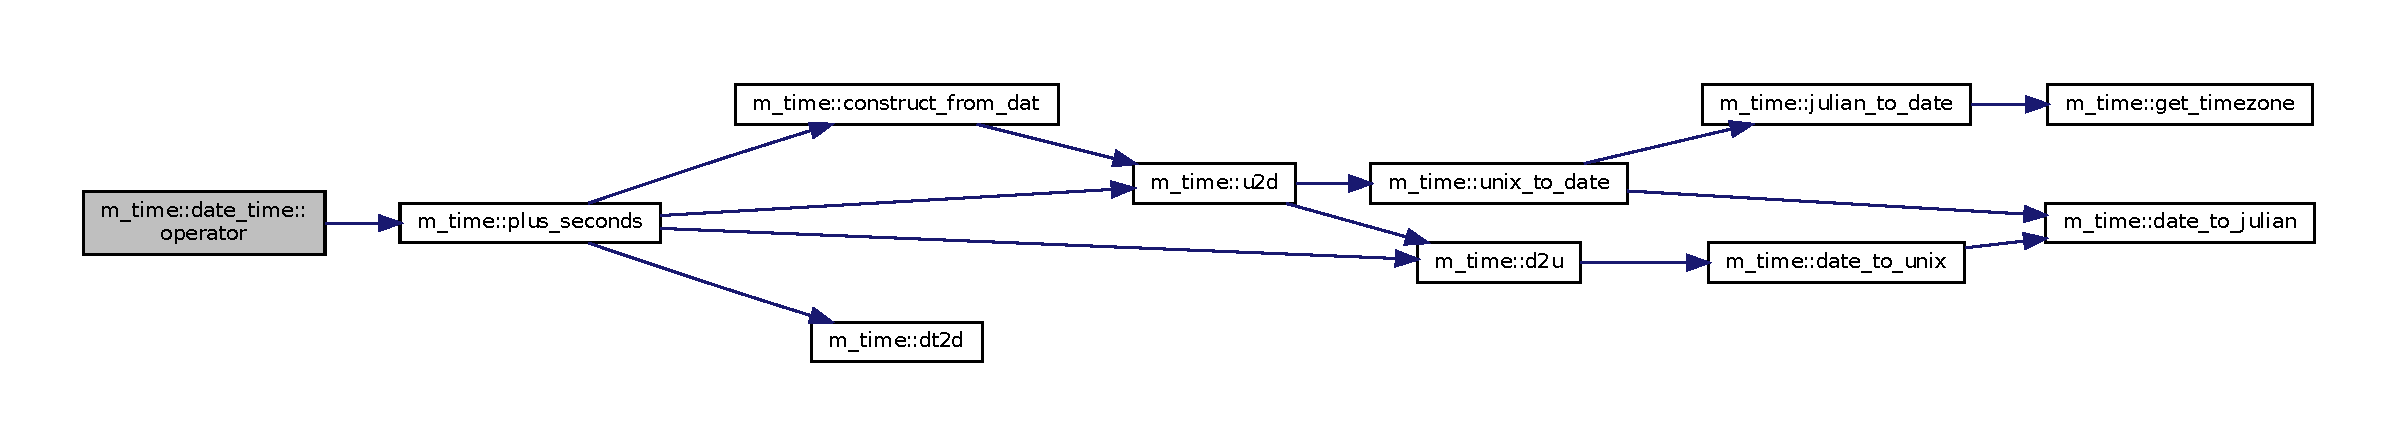
\includegraphics[width=350pt]{structm__time_1_1date__time_ad51508db1d161547062f40dcd91f4e4b_cgraph}
\end{center}
\end{figure}
\mbox{\Hypertarget{structm__time_1_1date__time_a67028b37f0375d0209cb6379c59d99e5}\label{structm__time_1_1date__time_a67028b37f0375d0209cb6379c59d99e5}} 
\index{m\+\_\+time\+::date\+\_\+time@{m\+\_\+time\+::date\+\_\+time}!operator@{operator}}
\index{operator@{operator}!m\+\_\+time\+::date\+\_\+time@{m\+\_\+time\+::date\+\_\+time}}
\subsubsection{\texorpdfstring{operator()}{operator()}\hspace{0.1cm}{\footnotesize\ttfamily [2/9]}}
{\footnotesize\ttfamily generic m\+\_\+time\+::date\+\_\+time\+::operator (\begin{DoxyParamCaption}{ }\end{DoxyParamCaption})\hspace{0.3cm}{\ttfamily [private]}}



References m\+\_\+time\+::eq().

Here is the call graph for this function\+:\nopagebreak
\begin{figure}[H]
\begin{center}
\leavevmode
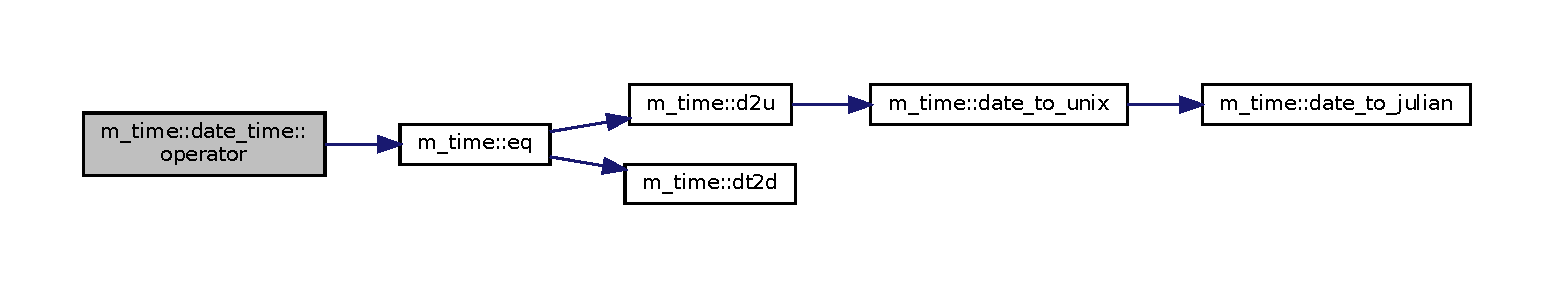
\includegraphics[width=350pt]{structm__time_1_1date__time_a67028b37f0375d0209cb6379c59d99e5_cgraph}
\end{center}
\end{figure}
\mbox{\Hypertarget{structm__time_1_1date__time_afd5a2b9837bc8d48eb244bd07c200c6a}\label{structm__time_1_1date__time_afd5a2b9837bc8d48eb244bd07c200c6a}} 
\index{m\+\_\+time\+::date\+\_\+time@{m\+\_\+time\+::date\+\_\+time}!operator@{operator}}
\index{operator@{operator}!m\+\_\+time\+::date\+\_\+time@{m\+\_\+time\+::date\+\_\+time}}
\subsubsection{\texorpdfstring{operator()}{operator()}\hspace{0.1cm}{\footnotesize\ttfamily [3/9]}}
{\footnotesize\ttfamily generic m\+\_\+time\+::date\+\_\+time\+::operator (\begin{DoxyParamCaption}{ }\end{DoxyParamCaption})\hspace{0.3cm}{\ttfamily [private]}}



References m\+\_\+time\+::lt().

Here is the call graph for this function\+:\nopagebreak
\begin{figure}[H]
\begin{center}
\leavevmode
\includegraphics[width=350pt]{structm__time_1_1date__time_afd5a2b9837bc8d48eb244bd07c200c6a_cgraph}
\end{center}
\end{figure}
\mbox{\Hypertarget{structm__time_1_1date__time_a1aa01f75ae1f67a4b3202febd56b462f}\label{structm__time_1_1date__time_a1aa01f75ae1f67a4b3202febd56b462f}} 
\index{m\+\_\+time\+::date\+\_\+time@{m\+\_\+time\+::date\+\_\+time}!operator@{operator}}
\index{operator@{operator}!m\+\_\+time\+::date\+\_\+time@{m\+\_\+time\+::date\+\_\+time}}
\subsubsection{\texorpdfstring{operator()}{operator()}\hspace{0.1cm}{\footnotesize\ttfamily [4/9]}}
{\footnotesize\ttfamily generic m\+\_\+time\+::date\+\_\+time\+::operator (\begin{DoxyParamCaption}{ }\end{DoxyParamCaption})\hspace{0.3cm}{\ttfamily [private]}}



References m\+\_\+time\+::gt().

Here is the call graph for this function\+:\nopagebreak
\begin{figure}[H]
\begin{center}
\leavevmode
\includegraphics[width=350pt]{structm__time_1_1date__time_a1aa01f75ae1f67a4b3202febd56b462f_cgraph}
\end{center}
\end{figure}
\mbox{\Hypertarget{structm__time_1_1date__time_a3961b17820108c6eb0037d11a03cfcd2}\label{structm__time_1_1date__time_a3961b17820108c6eb0037d11a03cfcd2}} 
\index{m\+\_\+time\+::date\+\_\+time@{m\+\_\+time\+::date\+\_\+time}!operator@{operator}}
\index{operator@{operator}!m\+\_\+time\+::date\+\_\+time@{m\+\_\+time\+::date\+\_\+time}}
\subsubsection{\texorpdfstring{operator()}{operator()}\hspace{0.1cm}{\footnotesize\ttfamily [5/9]}}
{\footnotesize\ttfamily generic m\+\_\+time\+::date\+\_\+time\+::operator (\begin{DoxyParamCaption}{ }\end{DoxyParamCaption})\hspace{0.3cm}{\ttfamily [private]}}



References m\+\_\+time\+::ge().

Here is the call graph for this function\+:\nopagebreak
\begin{figure}[H]
\begin{center}
\leavevmode
\includegraphics[width=350pt]{structm__time_1_1date__time_a3961b17820108c6eb0037d11a03cfcd2_cgraph}
\end{center}
\end{figure}
\mbox{\Hypertarget{structm__time_1_1date__time_add9b1c423294accdf967e22fa61a7796}\label{structm__time_1_1date__time_add9b1c423294accdf967e22fa61a7796}} 
\index{m\+\_\+time\+::date\+\_\+time@{m\+\_\+time\+::date\+\_\+time}!operator@{operator}}
\index{operator@{operator}!m\+\_\+time\+::date\+\_\+time@{m\+\_\+time\+::date\+\_\+time}}
\subsubsection{\texorpdfstring{operator()}{operator()}\hspace{0.1cm}{\footnotesize\ttfamily [6/9]}}
{\footnotesize\ttfamily generic m\+\_\+time\+::date\+\_\+time\+::operator (\begin{DoxyParamCaption}{ }\end{DoxyParamCaption})\hspace{0.3cm}{\ttfamily [private]}}



References m\+\_\+time\+::le().

Here is the call graph for this function\+:\nopagebreak
\begin{figure}[H]
\begin{center}
\leavevmode
\includegraphics[width=350pt]{structm__time_1_1date__time_add9b1c423294accdf967e22fa61a7796_cgraph}
\end{center}
\end{figure}
\mbox{\Hypertarget{structm__time_1_1date__time_af93a94ed420ca7ba08cc63c36e88459c}\label{structm__time_1_1date__time_af93a94ed420ca7ba08cc63c36e88459c}} 
\index{m\+\_\+time\+::date\+\_\+time@{m\+\_\+time\+::date\+\_\+time}!operator@{operator}}
\index{operator@{operator}!m\+\_\+time\+::date\+\_\+time@{m\+\_\+time\+::date\+\_\+time}}
\subsubsection{\texorpdfstring{operator()}{operator()}\hspace{0.1cm}{\footnotesize\ttfamily [7/9]}}
{\footnotesize\ttfamily generic m\+\_\+time\+::date\+\_\+time\+::operator (\begin{DoxyParamCaption}{ }\end{DoxyParamCaption})\hspace{0.3cm}{\ttfamily [private]}}



References m\+\_\+time\+::ne().

Here is the call graph for this function\+:\nopagebreak
\begin{figure}[H]
\begin{center}
\leavevmode
\includegraphics[width=350pt]{structm__time_1_1date__time_af93a94ed420ca7ba08cc63c36e88459c_cgraph}
\end{center}
\end{figure}
\mbox{\Hypertarget{structm__time_1_1date__time_affafbae65afa1e12c901241e641e4b1f}\label{structm__time_1_1date__time_affafbae65afa1e12c901241e641e4b1f}} 
\index{m\+\_\+time\+::date\+\_\+time@{m\+\_\+time\+::date\+\_\+time}!operator@{operator}}
\index{operator@{operator}!m\+\_\+time\+::date\+\_\+time@{m\+\_\+time\+::date\+\_\+time}}
\subsubsection{\texorpdfstring{operator()}{operator()}\hspace{0.1cm}{\footnotesize\ttfamily [8/9]}}
{\footnotesize\ttfamily generic m\+\_\+time\+::date\+\_\+time\+::operator (\begin{DoxyParamCaption}{ }\end{DoxyParamCaption})\hspace{0.3cm}{\ttfamily [private]}}



References m\+\_\+time\+::minus\+\_\+seconds().

Here is the call graph for this function\+:\nopagebreak
\begin{figure}[H]
\begin{center}
\leavevmode
\includegraphics[width=350pt]{structm__time_1_1date__time_affafbae65afa1e12c901241e641e4b1f_cgraph}
\end{center}
\end{figure}
\mbox{\Hypertarget{structm__time_1_1date__time_adc11c2984fd9dae163e44627a5e2a134}\label{structm__time_1_1date__time_adc11c2984fd9dae163e44627a5e2a134}} 
\index{m\+\_\+time\+::date\+\_\+time@{m\+\_\+time\+::date\+\_\+time}!operator@{operator}}
\index{operator@{operator}!m\+\_\+time\+::date\+\_\+time@{m\+\_\+time\+::date\+\_\+time}}
\subsubsection{\texorpdfstring{operator()}{operator()}\hspace{0.1cm}{\footnotesize\ttfamily [9/9]}}
{\footnotesize\ttfamily generic m\+\_\+time\+::date\+\_\+time\+::operator (\begin{DoxyParamCaption}{ }\end{DoxyParamCaption})\hspace{0.3cm}{\ttfamily [private]}}



References m\+\_\+time\+::construct\+\_\+from\+\_\+dat(), and m\+\_\+time\+::minus\+\_\+date\+\_\+time().

Here is the call graph for this function\+:\nopagebreak
\begin{figure}[H]
\begin{center}
\leavevmode
\includegraphics[width=350pt]{structm__time_1_1date__time_adc11c2984fd9dae163e44627a5e2a134_cgraph}
\end{center}
\end{figure}
\mbox{\Hypertarget{structm__time_1_1date__time_a0020bfaff4b78b7b0688dada7997d9f6}\label{structm__time_1_1date__time_a0020bfaff4b78b7b0688dada7997d9f6}} 
\index{m\+\_\+time\+::date\+\_\+time@{m\+\_\+time\+::date\+\_\+time}!ordinal@{ordinal}}
\index{ordinal@{ordinal}!m\+\_\+time\+::date\+\_\+time@{m\+\_\+time\+::date\+\_\+time}}
\subsubsection{\texorpdfstring{ordinal()}{ordinal()}}
{\footnotesize\ttfamily procedure m\+\_\+time\+::date\+\_\+time\+::ordinal (\begin{DoxyParamCaption}{ }\end{DoxyParamCaption})\hspace{0.3cm}{\ttfamily [private]}}

\mbox{\Hypertarget{structm__time_1_1date__time_a05e1950f16d81be0499b403b7e369b40}\label{structm__time_1_1date__time_a05e1950f16d81be0499b403b7e369b40}} 
\index{m\+\_\+time\+::date\+\_\+time@{m\+\_\+time\+::date\+\_\+time}!plus\+\_\+seconds@{plus\+\_\+seconds}}
\index{plus\+\_\+seconds@{plus\+\_\+seconds}!m\+\_\+time\+::date\+\_\+time@{m\+\_\+time\+::date\+\_\+time}}
\subsubsection{\texorpdfstring{plus\+\_\+seconds()}{plus\_seconds()}}
{\footnotesize\ttfamily procedure, private m\+\_\+time\+::date\+\_\+time\+::plus\+\_\+seconds (\begin{DoxyParamCaption}{ }\end{DoxyParamCaption})\hspace{0.3cm}{\ttfamily [private]}}

\mbox{\Hypertarget{structm__time_1_1date__time_abfb29551ce7b06e12ae947bac78cd345}\label{structm__time_1_1date__time_abfb29551ce7b06e12ae947bac78cd345}} 
\index{m\+\_\+time\+::date\+\_\+time@{m\+\_\+time\+::date\+\_\+time}!weekday@{weekday}}
\index{weekday@{weekday}!m\+\_\+time\+::date\+\_\+time@{m\+\_\+time\+::date\+\_\+time}}
\subsubsection{\texorpdfstring{weekday()}{weekday()}}
{\footnotesize\ttfamily procedure m\+\_\+time\+::date\+\_\+time\+::weekday (\begin{DoxyParamCaption}{ }\end{DoxyParamCaption})\hspace{0.3cm}{\ttfamily [private]}}



\subsection{Member Data Documentation}
\mbox{\Hypertarget{structm__time_1_1date__time_a7bfa953907e96e82128a4ab5eac0a33e}\label{structm__time_1_1date__time_a7bfa953907e96e82128a4ab5eac0a33e}} 
\index{m\+\_\+time\+::date\+\_\+time@{m\+\_\+time\+::date\+\_\+time}!day@{day}}
\index{day@{day}!m\+\_\+time\+::date\+\_\+time@{m\+\_\+time\+::date\+\_\+time}}
\subsubsection{\texorpdfstring{day}{day}}
{\footnotesize\ttfamily integer m\+\_\+time\+::date\+\_\+time\+::day =1\hspace{0.3cm}{\ttfamily [private]}}

\mbox{\Hypertarget{structm__time_1_1date__time_a95fab5ef1aea89d18411f26f34192f1a}\label{structm__time_1_1date__time_a95fab5ef1aea89d18411f26f34192f1a}} 
\index{m\+\_\+time\+::date\+\_\+time@{m\+\_\+time\+::date\+\_\+time}!hour@{hour}}
\index{hour@{hour}!m\+\_\+time\+::date\+\_\+time@{m\+\_\+time\+::date\+\_\+time}}
\subsubsection{\texorpdfstring{hour}{hour}}
{\footnotesize\ttfamily integer m\+\_\+time\+::date\+\_\+time\+::hour =0\hspace{0.3cm}{\ttfamily [private]}}

\mbox{\Hypertarget{structm__time_1_1date__time_a9a2f1be9348dd330a30ffd207c0791fc}\label{structm__time_1_1date__time_a9a2f1be9348dd330a30ffd207c0791fc}} 
\index{m\+\_\+time\+::date\+\_\+time@{m\+\_\+time\+::date\+\_\+time}!millisecond@{millisecond}}
\index{millisecond@{millisecond}!m\+\_\+time\+::date\+\_\+time@{m\+\_\+time\+::date\+\_\+time}}
\subsubsection{\texorpdfstring{millisecond}{millisecond}}
{\footnotesize\ttfamily integer m\+\_\+time\+::date\+\_\+time\+::millisecond =0\hspace{0.3cm}{\ttfamily [private]}}

\mbox{\Hypertarget{structm__time_1_1date__time_a9ac3edac50f8a4aae577b1c889404837}\label{structm__time_1_1date__time_a9ac3edac50f8a4aae577b1c889404837}} 
\index{m\+\_\+time\+::date\+\_\+time@{m\+\_\+time\+::date\+\_\+time}!minute@{minute}}
\index{minute@{minute}!m\+\_\+time\+::date\+\_\+time@{m\+\_\+time\+::date\+\_\+time}}
\subsubsection{\texorpdfstring{minute}{minute}}
{\footnotesize\ttfamily integer m\+\_\+time\+::date\+\_\+time\+::minute =0\hspace{0.3cm}{\ttfamily [private]}}

\mbox{\Hypertarget{structm__time_1_1date__time_aa0360a36979a7e0f621770379d432032}\label{structm__time_1_1date__time_aa0360a36979a7e0f621770379d432032}} 
\index{m\+\_\+time\+::date\+\_\+time@{m\+\_\+time\+::date\+\_\+time}!month@{month}}
\index{month@{month}!m\+\_\+time\+::date\+\_\+time@{m\+\_\+time\+::date\+\_\+time}}
\subsubsection{\texorpdfstring{month}{month}}
{\footnotesize\ttfamily integer m\+\_\+time\+::date\+\_\+time\+::month =1\hspace{0.3cm}{\ttfamily [private]}}

\mbox{\Hypertarget{structm__time_1_1date__time_a22161ace4be90b741a1600435588fc64}\label{structm__time_1_1date__time_a22161ace4be90b741a1600435588fc64}} 
\index{m\+\_\+time\+::date\+\_\+time@{m\+\_\+time\+::date\+\_\+time}!second@{second}}
\index{second@{second}!m\+\_\+time\+::date\+\_\+time@{m\+\_\+time\+::date\+\_\+time}}
\subsubsection{\texorpdfstring{second}{second}}
{\footnotesize\ttfamily integer m\+\_\+time\+::date\+\_\+time\+::second =0\hspace{0.3cm}{\ttfamily [private]}}

\mbox{\Hypertarget{structm__time_1_1date__time_a74edfe999538728025d729a7ce69fddc}\label{structm__time_1_1date__time_a74edfe999538728025d729a7ce69fddc}} 
\index{m\+\_\+time\+::date\+\_\+time@{m\+\_\+time\+::date\+\_\+time}!tz@{tz}}
\index{tz@{tz}!m\+\_\+time\+::date\+\_\+time@{m\+\_\+time\+::date\+\_\+time}}
\subsubsection{\texorpdfstring{tz}{tz}}
{\footnotesize\ttfamily integer m\+\_\+time\+::date\+\_\+time\+::tz =0\hspace{0.3cm}{\ttfamily [private]}}

\mbox{\Hypertarget{structm__time_1_1date__time_aadd87661407a53f0b50fe7fc47038f52}\label{structm__time_1_1date__time_aadd87661407a53f0b50fe7fc47038f52}} 
\index{m\+\_\+time\+::date\+\_\+time@{m\+\_\+time\+::date\+\_\+time}!year@{year}}
\index{year@{year}!m\+\_\+time\+::date\+\_\+time@{m\+\_\+time\+::date\+\_\+time}}
\subsubsection{\texorpdfstring{year}{year}}
{\footnotesize\ttfamily integer m\+\_\+time\+::date\+\_\+time\+::year =1970\hspace{0.3cm}{\ttfamily [private]}}



The documentation for this interface was generated from the following file\+:\begin{DoxyCompactItemize}
\item 
/home/urbanjs/venus/\+V600/github/\+M\+\_\+time/src/\mbox{\hyperlink{M__time_8f90}{M\+\_\+time.\+f90}}\end{DoxyCompactItemize}

\hypertarget{interfacem__time_1_1string__to__value}{}\section{m\+\_\+time\+:\+:string\+\_\+to\+\_\+value Interface Reference}
\label{interfacem__time_1_1string__to__value}\index{m\+\_\+time\+::string\+\_\+to\+\_\+value@{m\+\_\+time\+::string\+\_\+to\+\_\+value}}
\subsection*{Private Member Functions}
\begin{DoxyCompactItemize}
\item 
subroutine \mbox{\hyperlink{interfacem__time_1_1string__to__value_acbb157ca1468d2931a9fdd52581aeb96}{a2d}} (chars, valu, ierr, onerr)
\item 
subroutine \mbox{\hyperlink{interfacem__time_1_1string__to__value_a5fa7202ea5e4570e7ab54c7ec8188f57}{a2r}} (chars, valu, ierr)
\begin{DoxyCompactList}\small\item\em \subsubsection*{N\+A\+ME}

string\+\_\+to\+\_\+value(3f) -\/ \mbox{[}M\+\_\+strings\+:N\+U\+M\+E\+R\+IC\mbox{]} subroutine returns numeric value from string (L\+I\+C\+E\+N\+SE\+:PD) \end{DoxyCompactList}\item 
subroutine \mbox{\hyperlink{interfacem__time_1_1string__to__value_a6b07c7d16ad4033167209109583282c8}{a2i}} (chars, valu, ierr)
\end{DoxyCompactItemize}


\subsection{Member Function/\+Subroutine Documentation}
\mbox{\Hypertarget{interfacem__time_1_1string__to__value_acbb157ca1468d2931a9fdd52581aeb96}\label{interfacem__time_1_1string__to__value_acbb157ca1468d2931a9fdd52581aeb96}} 
\index{m\+\_\+time\+::string\+\_\+to\+\_\+value@{m\+\_\+time\+::string\+\_\+to\+\_\+value}!a2d@{a2d}}
\index{a2d@{a2d}!m\+\_\+time\+::string\+\_\+to\+\_\+value@{m\+\_\+time\+::string\+\_\+to\+\_\+value}}
\subsubsection{\texorpdfstring{a2d()}{a2d()}}
{\footnotesize\ttfamily subroutine m\+\_\+time\+::string\+\_\+to\+\_\+value\+::a2d (\begin{DoxyParamCaption}\item[{character(len=$\ast$), intent(in)}]{chars,  }\item[{doubleprecision, intent(out)}]{valu,  }\item[{integer, intent(out)}]{ierr,  }\item[{class($\ast$), intent(in), optional}]{onerr }\end{DoxyParamCaption})\hspace{0.3cm}{\ttfamily [private]}}

\mbox{\Hypertarget{interfacem__time_1_1string__to__value_a6b07c7d16ad4033167209109583282c8}\label{interfacem__time_1_1string__to__value_a6b07c7d16ad4033167209109583282c8}} 
\index{m\+\_\+time\+::string\+\_\+to\+\_\+value@{m\+\_\+time\+::string\+\_\+to\+\_\+value}!a2i@{a2i}}
\index{a2i@{a2i}!m\+\_\+time\+::string\+\_\+to\+\_\+value@{m\+\_\+time\+::string\+\_\+to\+\_\+value}}
\subsubsection{\texorpdfstring{a2i()}{a2i()}}
{\footnotesize\ttfamily subroutine m\+\_\+time\+::string\+\_\+to\+\_\+value\+::a2i (\begin{DoxyParamCaption}\item[{character(len=$\ast$), intent(in)}]{chars,  }\item[{integer, intent(out)}]{valu,  }\item[{integer, intent(out)}]{ierr }\end{DoxyParamCaption})\hspace{0.3cm}{\ttfamily [private]}}

\mbox{\Hypertarget{interfacem__time_1_1string__to__value_a5fa7202ea5e4570e7ab54c7ec8188f57}\label{interfacem__time_1_1string__to__value_a5fa7202ea5e4570e7ab54c7ec8188f57}} 
\index{m\+\_\+time\+::string\+\_\+to\+\_\+value@{m\+\_\+time\+::string\+\_\+to\+\_\+value}!a2r@{a2r}}
\index{a2r@{a2r}!m\+\_\+time\+::string\+\_\+to\+\_\+value@{m\+\_\+time\+::string\+\_\+to\+\_\+value}}
\subsubsection{\texorpdfstring{a2r()}{a2r()}}
{\footnotesize\ttfamily subroutine m\+\_\+time\+::string\+\_\+to\+\_\+value\+::a2r (\begin{DoxyParamCaption}\item[{character(len=$\ast$), intent(in)}]{chars,  }\item[{real, intent(out)}]{valu,  }\item[{integer, intent(out)}]{ierr }\end{DoxyParamCaption})\hspace{0.3cm}{\ttfamily [private]}}



\subsubsection*{N\+A\+ME}

string\+\_\+to\+\_\+value(3f) -\/ \mbox{[}M\+\_\+strings\+:N\+U\+M\+E\+R\+IC\mbox{]} subroutine returns numeric value from string (L\+I\+C\+E\+N\+SE\+:PD) 

\subsubsection*{S\+Y\+N\+O\+P\+S\+IS}

\begin{DoxyVerb}subroutine string_to_value(chars,valu,ierr)

 character(len=*),intent(in)              :: chars   ! input string
 integer|real|doubleprecision,intent(out) :: valu
 integer,intent(out)                      :: ierr
\end{DoxyVerb}
 \subsubsection*{D\+E\+S\+C\+R\+I\+P\+T\+I\+ON}

returns a numeric value from a numeric character string.

works with any g-\/format input, including integer, real, and exponential. If the input string begins with \char`\"{}\+B\char`\"{}, \char`\"{}\+Z\char`\"{}, or \char`\"{}\+O\char`\"{} and otherwise represents a positive whole number it is assumed to be a binary, hexadecimal, or octal value. If the string contains commas they are removed. If the string is of the form NN\+:M\+MM... or N\+N\+::\+M\+MM then NN is assumed to be the base of the whole number.

if an error occurs in the R\+E\+AD, I\+O\+S\+T\+AT is returned in I\+E\+RR and value is set to zero. if no error occurs, I\+E\+RR=0. \subsubsection*{O\+P\+T\+I\+O\+NS}

C\+H\+A\+RS input string to read numeric value from \subsubsection*{R\+E\+T\+U\+R\+NS}

V\+A\+LU numeric value returned. May be I\+N\+T\+E\+G\+ER, R\+E\+AL, or D\+O\+U\+B\+L\+E\+P\+R\+E\+C\+I\+S\+I\+ON. I\+E\+RR error flag (0 == no error) \subsubsection*{E\+X\+A\+M\+P\+LE}

\begin{DoxyVerb}Sample Program:

 program demo_string_to_value
 use M_strings, only: string_to_value
 character(len=80) :: string
    string=' -40.5e-2 '
    call string_to_value(string,value,ierr)
    write(*,*) 'value of string ['//trim(string)//'] is ',value
 end program demo_string_to_value
\end{DoxyVerb}
 \subsubsection*{A\+U\+T\+H\+OR}

John S. Urban \subsubsection*{L\+I\+C\+E\+N\+SE}

Public Domain 

The documentation for this interface was generated from the following file\+:\begin{DoxyCompactItemize}
\item 
/home/urbanjs/venus/\+V600/github/\+M\+\_\+time/src/\mbox{\hyperlink{M__time_8f90}{M\+\_\+time.\+f90}}\end{DoxyCompactItemize}

\hypertarget{interfacem__time_1_1v2s}{}\section{m\+\_\+time\+:\+:v2s Interface Reference}
\label{interfacem__time_1_1v2s}\index{m\+\_\+time\+::v2s@{m\+\_\+time\+::v2s}}
\subsection*{Private Member Functions}
\begin{DoxyCompactItemize}
\item 
character(len=\+:) function, allocatable \mbox{\hyperlink{interfacem__time_1_1v2s_ac96c5488b421f591abf5db4ab5aee7b0}{d2s}} (dvalue, fmt)
\begin{DoxyCompactList}\small\item\em \subsubsection*{N\+A\+ME}

v2s(3f) -\/ \mbox{[}M\+\_\+strings\+:N\+U\+M\+E\+R\+IC\mbox{]} return numeric string from a numeric value (L\+I\+C\+E\+N\+SE\+:PD) \end{DoxyCompactList}\item 
character(len=\+:) function, allocatable \mbox{\hyperlink{interfacem__time_1_1v2s_a5bc519244bd303a3dbad639743c0cff2}{r2s}} (rvalue, fmt)
\item 
character(len=\+:) function, allocatable \mbox{\hyperlink{interfacem__time_1_1v2s_aa950b277049afb5e6dac9c55c78d9539}{i2s}} (ivalue, fmt)
\item 
character(len=\+:) function, allocatable \mbox{\hyperlink{interfacem__time_1_1v2s_a6daa793a11022426b014474553d812c5}{l2s}} (lvalue, fmt)
\end{DoxyCompactItemize}


\subsection{Member Function/\+Subroutine Documentation}
\mbox{\Hypertarget{interfacem__time_1_1v2s_ac96c5488b421f591abf5db4ab5aee7b0}\label{interfacem__time_1_1v2s_ac96c5488b421f591abf5db4ab5aee7b0}} 
\index{m\+\_\+time\+::v2s@{m\+\_\+time\+::v2s}!d2s@{d2s}}
\index{d2s@{d2s}!m\+\_\+time\+::v2s@{m\+\_\+time\+::v2s}}
\subsubsection{\texorpdfstring{d2s()}{d2s()}}
{\footnotesize\ttfamily character(len=\+:) function, allocatable m\+\_\+time\+::v2s\+::d2s (\begin{DoxyParamCaption}\item[{doubleprecision, intent(in)}]{dvalue,  }\item[{character(len=$\ast$), intent(in), optional}]{fmt }\end{DoxyParamCaption})\hspace{0.3cm}{\ttfamily [private]}}



\subsubsection*{N\+A\+ME}

v2s(3f) -\/ \mbox{[}M\+\_\+strings\+:N\+U\+M\+E\+R\+IC\mbox{]} return numeric string from a numeric value (L\+I\+C\+E\+N\+SE\+:PD) 

\subsubsection*{S\+Y\+N\+O\+P\+S\+IS}

\begin{DoxyVerb}   function v2s(value) result(outstr)

    integer|real|doubleprecision|logical,intent(in ) :: value
    character(len=:),allocatable :: outstr
    character(len=*),optional,intent(in) :: fmt
\end{DoxyVerb}


\subsubsection*{D\+E\+S\+C\+R\+I\+P\+T\+I\+ON}

v2s(3f) returns a representation of a numeric value as a string when given a numeric value of type R\+E\+AL, D\+O\+U\+B\+L\+E\+P\+R\+E\+C\+I\+S\+I\+ON, I\+N\+T\+E\+G\+ER or L\+O\+G\+I\+C\+AL. It creates the strings using internal W\+R\+I\+T\+E() statements. Trailing zeros are removed from non-\/zero values, and the string is left-\/justified.

\subsubsection*{O\+P\+T\+I\+O\+NS}

V\+A\+L\+UE input value to be converted to a string F\+MT format can be explicitly given, but is limited to generating a string of eighty or less characters.

\subsubsection*{R\+E\+T\+U\+R\+NS}

O\+U\+T\+S\+TR returned string representing input value,

\subsubsection*{E\+X\+A\+M\+P\+LE}

\begin{DoxyVerb}Sample Program:

 program demo_v2s
 use M_strings, only: v2s
 write(*,*) 'The value of 3.0/4.0 is ['//v2s(3.0/4.0)//']'
 write(*,*) 'The value of 1234    is ['//v2s(1234)//']'
 write(*,*) 'The value of 0d0     is ['//v2s(0d0)//']'
 write(*,*) 'The value of .false. is ['//v2s(.false.)//']'
 write(*,*) 'The value of .true. is  ['//v2s(.true.)//']'
 end program demo_v2s

Expected output

 The value of 3.0/4.0 is [0.75]
 The value of 1234    is [1234]
 The value of 0d0     is [0]
 The value of .false. is [F]
 The value of .true. is  [T]
\end{DoxyVerb}


\subsubsection*{A\+U\+T\+H\+OR}

John S. Urban \subsubsection*{L\+I\+C\+E\+N\+SE}

Public Domain \mbox{\Hypertarget{interfacem__time_1_1v2s_aa950b277049afb5e6dac9c55c78d9539}\label{interfacem__time_1_1v2s_aa950b277049afb5e6dac9c55c78d9539}} 
\index{m\+\_\+time\+::v2s@{m\+\_\+time\+::v2s}!i2s@{i2s}}
\index{i2s@{i2s}!m\+\_\+time\+::v2s@{m\+\_\+time\+::v2s}}
\subsubsection{\texorpdfstring{i2s()}{i2s()}}
{\footnotesize\ttfamily character(len=\+:) function, allocatable m\+\_\+time\+::v2s\+::i2s (\begin{DoxyParamCaption}\item[{integer, intent(in)}]{ivalue,  }\item[{character(len=$\ast$), intent(in), optional}]{fmt }\end{DoxyParamCaption})\hspace{0.3cm}{\ttfamily [private]}}

\mbox{\Hypertarget{interfacem__time_1_1v2s_a6daa793a11022426b014474553d812c5}\label{interfacem__time_1_1v2s_a6daa793a11022426b014474553d812c5}} 
\index{m\+\_\+time\+::v2s@{m\+\_\+time\+::v2s}!l2s@{l2s}}
\index{l2s@{l2s}!m\+\_\+time\+::v2s@{m\+\_\+time\+::v2s}}
\subsubsection{\texorpdfstring{l2s()}{l2s()}}
{\footnotesize\ttfamily character(len=\+:) function, allocatable m\+\_\+time\+::v2s\+::l2s (\begin{DoxyParamCaption}\item[{logical, intent(in)}]{lvalue,  }\item[{character(len=$\ast$), intent(in), optional}]{fmt }\end{DoxyParamCaption})\hspace{0.3cm}{\ttfamily [private]}}

\mbox{\Hypertarget{interfacem__time_1_1v2s_a5bc519244bd303a3dbad639743c0cff2}\label{interfacem__time_1_1v2s_a5bc519244bd303a3dbad639743c0cff2}} 
\index{m\+\_\+time\+::v2s@{m\+\_\+time\+::v2s}!r2s@{r2s}}
\index{r2s@{r2s}!m\+\_\+time\+::v2s@{m\+\_\+time\+::v2s}}
\subsubsection{\texorpdfstring{r2s()}{r2s()}}
{\footnotesize\ttfamily character(len=\+:) function, allocatable m\+\_\+time\+::v2s\+::r2s (\begin{DoxyParamCaption}\item[{real, intent(in)}]{rvalue,  }\item[{character(len=$\ast$), intent(in), optional}]{fmt }\end{DoxyParamCaption})\hspace{0.3cm}{\ttfamily [private]}}



The documentation for this interface was generated from the following file\+:\begin{DoxyCompactItemize}
\item 
/home/urbanjs/venus/\+V600/github/\+M\+\_\+time/src/\mbox{\hyperlink{M__time_8f90}{M\+\_\+time.\+f90}}\end{DoxyCompactItemize}

\chapter{File Documentation}
\hypertarget{M__time_8f90}{}\section{/home/urbanjs/venus/\+V600/github/\+M\+\_\+time/src/\+M\+\_\+time.f90 File Reference}
\label{M__time_8f90}\index{/home/urbanjs/venus/\+V600/github/\+M\+\_\+time/src/\+M\+\_\+time.\+f90@{/home/urbanjs/venus/\+V600/github/\+M\+\_\+time/src/\+M\+\_\+time.\+f90}}
\subsection*{Modules}
\begin{DoxyCompactItemize}
\item 
module \mbox{\hyperlink{namespacem__time}{m\+\_\+time}}
\end{DoxyCompactItemize}
\subsection*{Functions/\+Subroutines}
\begin{DoxyCompactItemize}
\item 
subroutine, public \mbox{\hyperlink{namespacem__time_acfdc970b4154b0c15bd33727636e3992}{m\+\_\+time\+::date\+\_\+to\+\_\+julian}} (dat, julian, ierr)
\begin{DoxyCompactList}\small\item\em \subsubsection*{N\+A\+ME}

date\+\_\+to\+\_\+julian(3f) -\/ \mbox{[}M\+\_\+time\+:J\+U\+L\+I\+AN\mbox{]} converts D\+AT date-\/time array to Julian Date (L\+I\+C\+E\+N\+SE\+:PD) \end{DoxyCompactList}\item 
subroutine, public \mbox{\hyperlink{namespacem__time_abb44cf18cd0a3e420c20469efb056203}{m\+\_\+time\+::julian\+\_\+to\+\_\+date}} (julian, dat, ierr)
\begin{DoxyCompactList}\small\item\em \subsubsection*{N\+A\+ME}

julian\+\_\+to\+\_\+date(3f) -\/ \mbox{[}M\+\_\+time\+:J\+U\+L\+I\+AN\mbox{]} converts a J\+E\+D(\+Julian Ephemeris Date) to a D\+AT date-\/time array. (L\+I\+C\+E\+N\+SE\+:PD) \end{DoxyCompactList}\item 
subroutine, public \mbox{\hyperlink{namespacem__time_aed245c691853279ebf0ce899dec9caa9}{m\+\_\+time\+::date\+\_\+to\+\_\+unix}} (dat, unixtime, ierr)
\begin{DoxyCompactList}\small\item\em \subsubsection*{N\+A\+ME}

date\+\_\+to\+\_\+unix(3f) -\/ \mbox{[}M\+\_\+time\+:U\+N\+I\+X\+\_\+\+E\+P\+O\+CH\mbox{]} converts D\+AT date-\/time array to Unix Epoch Time (L\+I\+C\+E\+N\+SE\+:PD) \end{DoxyCompactList}\item 
subroutine, public \mbox{\hyperlink{namespacem__time_acc62ada23f8fa2fe67b428702fbcbf1c}{m\+\_\+time\+::unix\+\_\+to\+\_\+date}} (unixtime, dat, ierr)
\begin{DoxyCompactList}\small\item\em \subsubsection*{N\+A\+ME}

unix\+\_\+to\+\_\+date(3f) -\/ \mbox{[}M\+\_\+time\+:U\+N\+I\+X\+\_\+\+E\+P\+O\+CH\mbox{]} converts Unix Epoch Time to D\+AT date-\/time array (L\+I\+C\+E\+N\+SE\+:PD) \end{DoxyCompactList}\item 
integer function, public \mbox{\hyperlink{namespacem__time_a727dd77bbd4a5d0e3947c5d303845947}{m\+\_\+time\+::d2o}} (dat)
\begin{DoxyCompactList}\small\item\em \subsubsection*{N\+A\+ME}

d2o(3f) -\/ \mbox{[}M\+\_\+time\+:O\+R\+D\+I\+N\+A\+L\+\_\+\+D\+AY\mbox{]} converts D\+AT date-\/time array to Ordinal day (L\+I\+C\+E\+N\+SE\+:PD) \end{DoxyCompactList}\item 
integer function, public \mbox{\hyperlink{namespacem__time_ab8960d2aa60e134bcf77247d8b257963}{m\+\_\+time\+::ordinal\+\_\+seconds}} ()
\begin{DoxyCompactList}\small\item\em \subsubsection*{N\+A\+ME}

ordinal\+\_\+seconds(3f) -\/ \mbox{[}M\+\_\+time\+:O\+R\+D\+I\+N\+A\+L\+\_\+\+D\+AY\mbox{]} seconds since beginning of year (L\+I\+C\+E\+N\+SE\+:PD) \subsubsection*{S\+Y\+N\+O\+P\+S\+IS}\end{DoxyCompactList}\item 
subroutine, public \mbox{\hyperlink{namespacem__time_aa4dca4409bf20a011bb04988c1335d63}{m\+\_\+time\+::ordinal\+\_\+to\+\_\+date}} (yyyy, ddd, dat)
\begin{DoxyCompactList}\small\item\em \subsubsection*{N\+A\+ME}

ordinal\+\_\+to\+\_\+date(3f) -\/ \mbox{[}M\+\_\+time\+:O\+R\+D\+I\+N\+A\+L\+\_\+\+D\+AY\mbox{]} when given a valid year and day of the year returns the D\+AT array for the date (L\+I\+C\+E\+N\+SE\+:PD) \subsubsection*{S\+Y\+N\+O\+P\+S\+IS}\end{DoxyCompactList}\item 
integer function, dimension(8), public \mbox{\hyperlink{namespacem__time_a55e2cb9efc9d4d209ae2864f073d4f19}{m\+\_\+time\+::o2d}} (ordinal, year)
\begin{DoxyCompactList}\small\item\em \subsubsection*{N\+A\+ME}

o2d(3f) -\/ \mbox{[}M\+\_\+time\+:O\+R\+D\+I\+N\+A\+L\+\_\+\+D\+AY\mbox{]} converts Ordinal day to D\+AT date-\/time array (L\+I\+C\+E\+N\+SE\+:PD) \end{DoxyCompactList}\item 
character(len=\+:) function, allocatable, public \mbox{\hyperlink{namespacem__time_a6f28cf00e4998bb50bb503f5e4bd3f77}{m\+\_\+time\+::v2mo}} (imonth)
\begin{DoxyCompactList}\small\item\em \subsubsection*{N\+A\+ME}

v2mo(3f) -\/ \mbox{[}M\+\_\+time\+:M\+O\+N\+T\+H\+\_\+\+N\+A\+ME\mbox{]} returns the month name of a Common month number (L\+I\+C\+E\+N\+SE\+:PD) \end{DoxyCompactList}\item 
integer function, dimension(8), public \mbox{\hyperlink{namespacem__time_a8188c7ed4e592c4f2388d28c75486726}{m\+\_\+time\+::mo2d}} (month\+\_\+name, year)
\begin{DoxyCompactList}\small\item\em \subsubsection*{N\+A\+ME}

mo2d(3f) -\/ \mbox{[}M\+\_\+time\+:M\+O\+N\+T\+H\+\_\+\+N\+A\+ME\mbox{]} given month name return D\+AT date-\/time array for beginning of that month in specified year (L\+I\+C\+E\+N\+SE\+:PD) \end{DoxyCompactList}\item 
integer function, public \mbox{\hyperlink{namespacem__time_ad7bf0886754757e8961e562f06cf3bb7}{m\+\_\+time\+::mo2v}} (month\+\_\+name)
\begin{DoxyCompactList}\small\item\em \subsubsection*{N\+A\+ME}

mo2v(3f) -\/ \mbox{[}M\+\_\+time\+:M\+O\+N\+T\+H\+\_\+\+N\+A\+ME\mbox{]} given month name return month number (1-\/12) of that month (L\+I\+C\+E\+N\+SE\+:PD) \end{DoxyCompactList}\item 
character(len=\+:) function, allocatable, public \mbox{\hyperlink{namespacem__time_a6b5e87be0e510ff268c1ecfbf67a3bdb}{m\+\_\+time\+::now}} (format)
\begin{DoxyCompactList}\small\item\em \subsubsection*{N\+A\+ME}

now(3f) -\/ \mbox{[}M\+\_\+time\+:D\+A\+T\+E\+\_\+\+P\+R\+I\+N\+T\+I\+NG\mbox{]} return string representing current time given format (L\+I\+C\+E\+N\+SE\+:PD) \end{DoxyCompactList}\item 
character(len=\+:) function, allocatable, public \mbox{\hyperlink{namespacem__time_a2cb84c9b8af4f395b76aed76e1431328}{m\+\_\+time\+::fmtdate}} (values, format)
\begin{DoxyCompactList}\small\item\em \subsubsection*{N\+A\+ME}

fmtdate(3f) -\/ \mbox{[}M\+\_\+time\+:D\+A\+T\+E\+\_\+\+P\+R\+I\+N\+T\+I\+NG\mbox{]} given D\+AT date-\/time array return date as string using specified format (L\+I\+C\+E\+N\+SE\+:PD) \end{DoxyCompactList}\item 
subroutine, public \mbox{\hyperlink{namespacem__time_a914927f70fb9495af1be2e484b967111}{m\+\_\+time\+::fmtdate\+\_\+usage}} (indent)
\begin{DoxyCompactList}\small\item\em \subsubsection*{N\+A\+ME}

fmtdate\+\_\+usage(3f) -\/ \mbox{[}M\+\_\+time\+:D\+A\+T\+E\+\_\+\+P\+R\+I\+N\+T\+I\+NG\mbox{]} display macros recognized by fmtdate(3f) and now(3f) (L\+I\+C\+E\+N\+SE\+:PD) \end{DoxyCompactList}\item 
subroutine, public \mbox{\hyperlink{namespacem__time_aa5198c7aa4f3d8411c8ce93046ce3794}{m\+\_\+time\+::guessdate}} (datestring, dat, ier)
\begin{DoxyCompactList}\small\item\em \subsubsection*{N\+A\+ME}

guessdate(3f) -\/ \mbox{[}M\+\_\+time\+:R\+E\+A\+D\+I\+N\+G\+\_\+\+D\+A\+T\+ES\mbox{]} reads in a date, in various formats (L\+I\+C\+E\+N\+SE\+:PD) \end{DoxyCompactList}\item 
subroutine, public \mbox{\hyperlink{namespacem__time_adfda8a89820b8d0ad4581a14896e4ce5}{m\+\_\+time\+::dow}} (values, weekday, day, ierr)
\begin{DoxyCompactList}\small\item\em \subsubsection*{N\+A\+ME}

dow(3f) -\/ \mbox{[}M\+\_\+time\+:D\+A\+Y\+\_\+\+O\+F\+\_\+\+W\+E\+EK\mbox{]} given a date-\/time array D\+AT return the day of the week (L\+I\+C\+E\+N\+SE\+:PD) \end{DoxyCompactList}\item 
subroutine, public \mbox{\hyperlink{namespacem__time_ad4ff99ad6f6d5282c4b65ad636a2a627}{m\+\_\+time\+::d2w}} (dat, iso\+\_\+year, iso\+\_\+week, iso\+\_\+weekday, iso\+\_\+name)
\begin{DoxyCompactList}\small\item\em \subsubsection*{N\+A\+ME}

d2w(3f) -\/ \mbox{[}M\+\_\+time\+:W\+E\+E\+K\+\_\+\+O\+F\+\_\+\+Y\+E\+AR\mbox{]} calculate iso-\/8601 Week-\/numbering year date yyyy-\/\+Www-\/d given D\+AT date-\/time array (L\+I\+C\+E\+N\+SE\+:PD) \end{DoxyCompactList}\item 
integer function \mbox{\hyperlink{M__time_8f90_a4a68c5e906616f64da0c3d165fc41479}{uncorrected\+\_\+week\+\_\+of\+\_\+year}} (datin)
\item 
subroutine, public \mbox{\hyperlink{namespacem__time_ac0ec48db8d508bfa23fe4b20c9d1c5a3}{m\+\_\+time\+::w2d}} (iso\+\_\+year, iso\+\_\+week, iso\+\_\+weekday, dat)
\begin{DoxyCompactList}\small\item\em \subsubsection*{N\+A\+ME}

w2d(3f) -\/ \mbox{[}M\+\_\+time\+:W\+E\+E\+K\+\_\+\+O\+F\+\_\+\+Y\+E\+AR\mbox{]} calculate D\+AT date-\/time array from iso-\/8601 Week-\/numbering year date yyyy-\/\+Www-\/d (L\+I\+C\+E\+N\+SE\+:PD) \end{DoxyCompactList}\item 
subroutine, public \mbox{\hyperlink{namespacem__time_a0fe7540912df30d3578f3c469413aea8}{m\+\_\+time\+::box\+\_\+month}} (dat, calen)
\begin{DoxyCompactList}\small\item\em \subsubsection*{N\+A\+ME}

box\+\_\+month(3f) -\/ \mbox{[}M\+\_\+time\+:D\+A\+T\+E\+\_\+\+P\+R\+I\+N\+T\+I\+NG\mbox{]} create specified month in a character array (L\+I\+C\+E\+N\+SE\+:PD) \end{DoxyCompactList}\item 
real(kind=realtime) function, public \mbox{\hyperlink{namespacem__time_a3fccc53c2650104eff084c7998d18f54}{m\+\_\+time\+::d2j}} (dat)
\begin{DoxyCompactList}\small\item\em \subsubsection*{N\+A\+ME}

d2j(3f) -\/ \mbox{[}M\+\_\+time\+:J\+U\+L\+I\+AN\mbox{]} given D\+AT date-\/time array returns Julian Date (L\+I\+C\+E\+N\+SE\+:PD) \end{DoxyCompactList}\item 
integer function, dimension(8), public \mbox{\hyperlink{namespacem__time_a3ad5cad6df02c53e0429c3602a072e3c}{m\+\_\+time\+::j2d}} (julian)
\begin{DoxyCompactList}\small\item\em \subsubsection*{N\+A\+ME}

j2d(3f) -\/ \mbox{[}M\+\_\+time\+:J\+U\+L\+I\+AN\mbox{]} given a J\+ED (Julian Ephemeris Date) returns a date-\/time array D\+AT. (L\+I\+C\+E\+N\+SE\+:PD) \end{DoxyCompactList}\item 
real(kind=realtime) function, public \mbox{\hyperlink{namespacem__time_a1506e2889a156387df4481ed0534be81}{m\+\_\+time\+::d2u}} (dat)
\begin{DoxyCompactList}\small\item\em \subsubsection*{N\+A\+ME}

d2u(3f) -\/ \mbox{[}M\+\_\+time\+:U\+N\+I\+X\+\_\+\+E\+P\+O\+CH\mbox{]} given D\+AT date-\/time array returns Unix Epoch Time (U\+ET starts at 0000 on 1 Jan. 1970, U\+TC) (L\+I\+C\+E\+N\+SE\+:PD) \end{DoxyCompactList}\item 
integer function, dimension(8), public \mbox{\hyperlink{namespacem__time_a083bc231f8ba1879d7f86ab424e77d6c}{m\+\_\+time\+::u2d}} (unixtime)
\begin{DoxyCompactList}\small\item\em \subsubsection*{N\+A\+ME}

u2d(3f) -\/ \mbox{[}M\+\_\+time\+:U\+N\+I\+X\+\_\+\+E\+P\+O\+CH\mbox{]} given Unix Epoch Time returns D\+AT date-\/time array (L\+I\+C\+E\+N\+SE\+:PD) \end{DoxyCompactList}\item 
integer function \mbox{\hyperlink{namespacem__time_a7903410a1d28bcdf3d33ab0c2d74b124}{m\+\_\+time\+::get\+\_\+timezone}} ()
\item 
character(len=\+:) function, allocatable, public \mbox{\hyperlink{namespacem__time_a7788285d79b8d58323b05e9a30a2d992}{m\+\_\+time\+::sec2days}} (seconds, crop)
\begin{DoxyCompactList}\small\item\em \subsubsection*{N\+A\+ME}

sec2days(3f) -\/ \mbox{[}M\+\_\+time\+:D\+U\+R\+A\+T\+I\+ON\mbox{]} convert seconds to string of form dd-\/hh\+:mm\+:ss (L\+I\+C\+E\+N\+SE\+:PD) \end{DoxyCompactList}\item 
real(kind=realtime) function, public \mbox{\hyperlink{namespacem__time_a99393c7906f1989f90ece03969224938}{m\+\_\+time\+::days2sec}} (str)
\begin{DoxyCompactList}\small\item\em \subsubsection*{N\+A\+ME}

days2sec(3f) -\/ \mbox{[}M\+\_\+time\+:D\+U\+R\+A\+T\+I\+ON\mbox{]} convert string of form \mbox{[}\mbox{[}-\/\mbox{]}dd-\/\mbox{]}hh\+:mm\+:ss.\+nn to seconds (L\+I\+C\+E\+N\+SE\+:PD) \end{DoxyCompactList}\item 
character(len=\+:) function, allocatable, public \mbox{\hyperlink{namespacem__time_ab8a976e2f113cc38b6df80974cee55dc}{m\+\_\+time\+::phase\+\_\+of\+\_\+moon}} (datin)
\begin{DoxyCompactList}\small\item\em \subsubsection*{N\+A\+ME}

phase\+\_\+of\+\_\+moon(3f) -\/ \mbox{[}M\+\_\+time\+:A\+S\+T\+R\+O\+L\+O\+G\+I\+C\+AL\mbox{]} return name for phase of moon for given date (L\+I\+C\+E\+N\+SE\+:PD) \subsubsection*{S\+Y\+N\+O\+P\+S\+IS}\end{DoxyCompactList}\item 
integer function, public \mbox{\hyperlink{namespacem__time_a702b39998a769b8f60070c0bec975ee2}{m\+\_\+time\+::moon\+\_\+fullness}} (datin)
\begin{DoxyCompactList}\small\item\em \subsubsection*{N\+A\+ME}

moon\+\_\+fullness(3f) -\/ \mbox{[}M\+\_\+time\+:A\+S\+T\+R\+O\+L\+O\+G\+I\+C\+AL\mbox{]} return percentage of moon phase from new to full (L\+I\+C\+E\+N\+SE\+:PD) \subsubsection*{S\+Y\+N\+O\+P\+S\+IS}\end{DoxyCompactList}\item 
subroutine, public \mbox{\hyperlink{namespacem__time_a5ccb70e20160fcf26bb403dbff1f138a}{m\+\_\+time\+::easter}} (year, dat)
\begin{DoxyCompactList}\small\item\em \subsubsection*{N\+A\+ME}

easter(3f) -\/ \mbox{[}M\+\_\+time\+:A\+S\+T\+R\+O\+L\+O\+G\+I\+C\+AL\mbox{]} calculate date for Easter given a year (L\+I\+C\+E\+N\+SE\+:PD) \end{DoxyCompactList}\item 
subroutine, public \mbox{\hyperlink{namespacem__time_a7c5d028ae1e1e01162ffc7bb55dcbbb1}{m\+\_\+time\+::system\+\_\+sleep}} (seconds)
\begin{DoxyCompactList}\small\item\em \subsubsection*{N\+A\+ME}

system\+\_\+sleep(3f) -\/ \mbox{[}M\+\_\+time\+:C\+\_\+\+I\+N\+T\+E\+R\+F\+A\+CE\mbox{]} call C sleep(3c) or usleep(3c) procedure (L\+I\+C\+E\+N\+SE\+:PD) \subsubsection*{S\+Y\+N\+O\+P\+S\+IS}\end{DoxyCompactList}\item 
subroutine, private \mbox{\hyperlink{namespacem__time_af558bfc1fd5b13a6b879b3969866956f}{m\+\_\+time\+::call\+\_\+sleep}} (wait\+\_\+seconds)
\item 
subroutine, private \mbox{\hyperlink{namespacem__time_ae63783f7479d2f5093c8031d38ce4304}{m\+\_\+time\+::call\+\_\+usleep}} (wait\+\_\+seconds)
\item 
character(len=\+:) function, allocatable \mbox{\hyperlink{M__time_8f90_a09223e2da0c23850fad035407582fd68}{now\+\_\+ex}} (format)
\end{DoxyCompactItemize}
\subsection*{Variables}
\begin{DoxyCompactItemize}
\item 
integer, parameter, public \mbox{\hyperlink{namespacem__time_ac10ea9e8d59ec74eaa7d89f2517d7422}{m\+\_\+time\+::realtime}} =kind(0.\+0d0)
\item 
real(kind=realtime), parameter, private \mbox{\hyperlink{namespacem__time_a48130b5a95a3f2e776269dcee1426797}{m\+\_\+time\+::secday}} =86400.\+0d0
\item 
real(kind=realtime), parameter, public \mbox{\hyperlink{namespacem__time_a9fe6fbb44e2779a2fcf96fba36c08918}{m\+\_\+time\+::dt\+\_\+minute}} =60.\+0d0
\item 
real(kind=realtime), parameter, public \mbox{\hyperlink{namespacem__time_aa0ca2172092f5e7dcc9b8524e6516fd8}{m\+\_\+time\+::dt\+\_\+hour}} =3600.\+0d0
\item 
real(kind=realtime), parameter, public \mbox{\hyperlink{namespacem__time_a97725f8d657c24badff19a794f323a6b}{m\+\_\+time\+::dt\+\_\+day}} =86400.\+0d0
\item 
real(kind=realtime), parameter, public \mbox{\hyperlink{namespacem__time_a3d53519e90264faccdae67e389ffc003}{m\+\_\+time\+::dt\+\_\+week}} =dt\+\_\+day$\ast$7.\+0d0
\end{DoxyCompactItemize}


\subsection{Function/\+Subroutine Documentation}
\mbox{\Hypertarget{M__time_8f90_a09223e2da0c23850fad035407582fd68}\label{M__time_8f90_a09223e2da0c23850fad035407582fd68}} 
\index{M\+\_\+time.\+f90@{M\+\_\+time.\+f90}!now\+\_\+ex@{now\+\_\+ex}}
\index{now\+\_\+ex@{now\+\_\+ex}!M\+\_\+time.\+f90@{M\+\_\+time.\+f90}}
\subsubsection{\texorpdfstring{now\+\_\+ex()}{now\_ex()}}
{\footnotesize\ttfamily character(len=\+:) function, allocatable now\+\_\+ex (\begin{DoxyParamCaption}\item[{character(len=$\ast$), intent(in), optional}]{format }\end{DoxyParamCaption})\hspace{0.3cm}{\ttfamily [private]}}



References m\+\_\+time\+::now().

Here is the call graph for this function\+:\nopagebreak
\begin{figure}[H]
\begin{center}
\leavevmode
\includegraphics[width=350pt]{M__time_8f90_a09223e2da0c23850fad035407582fd68_cgraph}
\end{center}
\end{figure}
\mbox{\Hypertarget{M__time_8f90_a4a68c5e906616f64da0c3d165fc41479}\label{M__time_8f90_a4a68c5e906616f64da0c3d165fc41479}} 
\index{M\+\_\+time.\+f90@{M\+\_\+time.\+f90}!uncorrected\+\_\+week\+\_\+of\+\_\+year@{uncorrected\+\_\+week\+\_\+of\+\_\+year}}
\index{uncorrected\+\_\+week\+\_\+of\+\_\+year@{uncorrected\+\_\+week\+\_\+of\+\_\+year}!M\+\_\+time.\+f90@{M\+\_\+time.\+f90}}
\subsubsection{\texorpdfstring{uncorrected\+\_\+week\+\_\+of\+\_\+year()}{uncorrected\_week\_of\_year()}}
{\footnotesize\ttfamily integer function d2w\+::uncorrected\+\_\+week\+\_\+of\+\_\+year (\begin{DoxyParamCaption}\item[{integer, dimension(8), intent(in)}]{datin }\end{DoxyParamCaption})\hspace{0.3cm}{\ttfamily [private]}}



References m\+\_\+time\+::d2o(), and m\+\_\+time\+::dow().

Here is the call graph for this function\+:\nopagebreak
\begin{figure}[H]
\begin{center}
\leavevmode
\includegraphics[width=350pt]{M__time_8f90_a4a68c5e906616f64da0c3d165fc41479_cgraph}
\end{center}
\end{figure}
Here is the caller graph for this function\+:\nopagebreak
\begin{figure}[H]
\begin{center}
\leavevmode
\includegraphics[width=350pt]{M__time_8f90_a4a68c5e906616f64da0c3d165fc41479_icgraph}
\end{center}
\end{figure}

\doxysection{/home/runner/work/\+M\+\_\+time/\+M\+\_\+time/src/mainpage.txt File Reference}
\hypertarget{mainpage_8txt}{}\label{mainpage_8txt}\index{/home/runner/work/M\_time/M\_time/src/mainpage.txt@{/home/runner/work/M\_time/M\_time/src/mainpage.txt}}

%--- End generated contents ---

% Index
\backmatter
\newpage
\phantomsection
\clearemptydoublepage
\addcontentsline{toc}{chapter}{Index}
\printindex

\end{document}
